\documentclass[a4paper, 12pt]{article}
\usepackage[T1]{fontenc}
\usepackage{lmodern}
\usepackage{color}
\usepackage{amsfonts}
\usepackage{epstopdf}
%\documentclass{book}
\usepackage{hyperref}
\usepackage[brazil]{babel}
\usepackage{amssymb}
\usepackage[utf8]{inputenc}
\usepackage{amsmath}
\usepackage{indentfirst}
\usepackage{graphicx}
\usepackage{multicol,lipsum}
\usepackage[a4paper,
top=3cm, left=3cm, bottom=3cm, right=3cm]{geometry}
\usepackage{setspace}
\usepackage{multirow}
\usepackage{float}
\usepackage[dvipsnames]{xcolor}
\usepackage[table]{xcolor}
%\usepackage{pdflscape}
\usepackage[DIV=15]{typearea}
\usepackage[nottoc]{tocbibind}
\usepackage[sort,numbers]{natbib}
%\usepackage{cite}
\usepackage[utf8]{inputenc}
\usepackage[T1]{fontenc}
\usepackage{lmodern}
\usepackage{graphicx}
\usepackage{color}
\usepackage{hyperref}
\usepackage{amsmath}
\usepackage{amsfonts}
\usepackage{epstopdf}
\usepackage[table]{xcolor}


\documentclass[letterpaper]{article}
% bib pack %%%%%%%%%%%%%%%%%%%%%%%%%%%%%%%%%%%%%%%%%%%%%%%%%%%%%%%%%%%%%%%%%%%%%
\usepackage[utf8]{inputenc}
\usepackage{geometry}
    \geometry{left=3cm,right=2cm,top=2cm,bottom=2cm}
%
\usepackage[spanish]{babel}
%
\usepackage[fixlanguage]{babelbib}
    \bibliographystyle{babunsrt}
%
\usepackage{url}

\begin{document}
%\maketitle

\begin{titlepage}
	\begin{center}
		

\vspace{10pt}
%\begin{figure}[H][!ht]
%\centering
%
\includegraphics{puc-rio-logo.png}

%\end{figure}
\begin{figure}
\centering

\includegraphics{imagens/puc-rio-logo.png}
\end{figure}
\huge{Circuitos Elétricos e Eletrônicos II}
        \vspace{70pt}
        
		\textbf{ENG4421}
        \vspace{20pt}
		\textbf{\large{\\Projeto G3}}
        \vspace{20pt}
        \textbf{\large{\\Respota em Frequência: Projeto de Afinador de Cordas de Violão}}
		\vspace{65pt}
		
	\end{center}
	
	\begin{flushleft}
		\begin{tabbing}
			Alunos\qquad\qquad\=\>Paloma Sette - 1621595 \\
            \>Luigi Gosling - 1811556 \\
            \>João Vitor Dias  - 1911231 \\
                
			Professor\>Guilherme Temporão\\
	\end{tabbing}
		  
	\end{flushleft}
	\begin{center}
		%\vspace{\fill}
            \vspace{225pt}
		Rio de Janeiro, 30 de Novembro de 2024
	\end{center}
\end{titlepage}
%%%%%%%%%%%%%%%%%%%%%%%%%%%%%%%%%%%%%%%%%%%%%%%%%%%%%%%%%%%

\newpage


\newpage
\tableofcontents
\thispagestyle{empty}

\newpage
\listoffigures
\thispagestyle{empty}

\newpage
\pagenumbering{arabic}

%%%%%%%%%%%%%%%%%%%%%%%%%%%%%%%%%%%%%%%%%%%%%%%%%%%%%%%%%
%%%%%%%%%%%%%%%%%%%%%%%%%%%%%%%%%%%%%%%%%%%%%%%%%%%equ

\section{Introdução}
O projeto em questão busca o desenvolvimento de um circuito eletrônico que simula um afinador de cordas de violão. Esse tipo de circuito é capaz de identificar a frequência de um sinal de entrada (representando a vibração de uma corda), determinando se a frequência corresponde ao valor esperado para a nota “lá” (440 Hz), padrão de afinação musical. Com a crescente aplicação de circuitos de análise de frequência em dispositivos de áudio e instrumentos musicais, esse projeto apresenta um estudo prático do uso de filtros e comparadores para discriminação de sinais com precisão.\\

No afinador tradicional de instrumentos, LEDs ou displays visuais indicam ao músico se a corda está afinada ou necessita de ajuste. Neste projeto, utiliza-se um sistema com três LEDs (verde, vermelho e amarelo) para indicar se a frequência da corda está dentro do intervalo de afinação desejado, acima ou abaixo do valor de referência. Através da análise e interpretação do sinal senoidal de entrada, o circuito identifica se a frequência está entre 435 Hz e 445 Hz (corda afinada), abaixo de 435 Hz (corda desafinada para baixo), ou acima de 445 Hz (corda desafinada para cima).

\newpage
\section{Objetivo}
O objetivo deste projeto é projetar, simular e documentar um circuito eletrônico que, ao receber um sinal senoidal de entrada com frequência variável, identifica se essa frequência corresponde ao intervalo de afinação da nota “lá” (440 Hz). A saída do circuito aciona LEDs indicadores que apresentam o status da afinação da frequência conforme as condições que serão descritas adiante.\\

Para atingir esses objetivos, o projeto utiliza técnicas de filtragem de frequência e comparação de sinais, implementando filtros \textbf{passa-baixa}, \textbf{passa-alta} e \textbf{passa-banda} em conjunto com comparadores. A montagem e simulação do circuito são realizadas no software LTspice, que permite a análise detalhada do comportamento do sistema e a verificação das condições para acionamento de cada LED. Ao final, espera-se um circuito funcional que consiga discriminar as frequências de entrada e fornecer a resposta visual de afinação correta.


\section{Metodologia}

\begin{enumerate}
    \item \textbf{Análise de Requisitos}:
    \begin{itemize}
    \item Precisaremos utilizar 3 LEDs, verde, amarelo e vermelho, cujo comportamento deverá ser:
    \begin{itemize}
        \item \textbf{LED Verde}: Acende se a frequência estiver entre 435 Hz e 445 Hz, indicando que a corda está afinada.
        \item \textbf{LED Amarelo}: Acende se a frequência estiver abaixo de 435 Hz, indicando que a corda está desafinada para baixo.
        \item \textbf{LED Vermelho}: Acende se a frequência estiver acima de 445 Hz, indicando que a corda está desafinada para cima.
    \end{itemize}
    \item O circuito vai receber um sinal senoidal de entrada representando a frequência que queremos analisar.
    
\end{itemize}
\item \textbf{Componentes Permitidos, além dos necessários}:
\begin{itemize}
    \item  2(duas) fontes DC de 12V, resistores, capacitores, indutores, amplificadores operacionais reais, diodos reais e transistores BJT ou FET (somente modelos de dispositivos reais).
\end{itemize}

\item \textbf{Planejamento do Circuito:}

\begin{itemize}
    \item Precisamos de uma forma de \textbf{filtrar e comparar} a frequência de entrada com os limites estabelecidos (435 Hz e 445 Hz).
    \item Amplificadores operacionais são usados para criar filtros e comparadores.
    \item Filtros \textbf{passa-banda } são utilizados para isolar a faixa de frequência entre 435 Hz e 445 Hz. Filtros \textbf{passa-baixa} e \textbf{passa-alta} são usados para identificar as frequências abaixo de 435 Hz e acima de 445 Hz.
    \item \textbf{Comparadores de frequência} são configurados com amplificadores operacionais para acionar cada LED com base na faixa de frequência detectada.
\end{itemize}
\end{enumerate}

\subsection{Filtros Ativos vs. Filtros Passivos}
\subsubsection{Comparação entre Filtros}

Filtros passivos são construídos apenas com componentes passivos, como resistores, capacitores e indutores. Eles apresentam simplicidade de construção e não requerem fontes de energia adicionais. Contudo, possuem limitações significativas, como ganho inferior a 1 (sempre atenuam o sinal) e sensibilidade à carga conectada à saída. Além disso, filtros passivos podem ter dificuldades em alcançar altos valores de fator de qualidade ($Q$), o que restringe seu desempenho em aplicações que exigem filtragem precisa.\\

Por outro lado, filtros ativos utilizam amplificadores operacionais em conjunto com componentes passivos. Isso permite que eles superem as limitações de ganho dos filtros passivos, proporcionando amplificação do sinal e maior flexibilidade no ajuste das características de frequência. Além disso, os filtros ativos são menos sensíveis às condições de carga devido à presença do estágio amplificador.

\subsubsection{Justificativa da Escolha}

Optou-se pelo uso de filtros ativos devido à sua capacidade de amplificar o sinal e proporcionar maior controle sobre os parâmetros do filtro, como frequência de corte e fator de qualidade (Q). Essa escolha é particularmente importante neste projeto, onde os filtros desempenham papel crítico na separação precisa de faixas de frequência. A implementação de filtros passivos seria inviável para os requisitos estabelecidos, especialmente devido à necessidade de Q elevado em certas frequências e à garantia de que o filtro funcione consistentemente, independentemente da carga conectada.

\subsection{Filtros Ativos Sallen-Key}

Os filtros Sallen-Key foram escolhidos devido à sua simplicidade de implementação e eficiência em aplicações de segunda ordem. Este tipo de arquitetura oferece uma solução robusta para projetar filtros com respostas controláveis, seja para baixa, alta ou banda passante.\\

A configuração Sallen-Key utiliza uma combinação de \textit{feedback} positivo e negativo para atingir o valor desejado de $Q$ e frequência de corte ($f_c$). Para filtros de segunda ordem, ela é particularmente eficaz na realização de curvas de resposta precisas, como Butterworth ou Chebyshev, dependendo dos valores dos componentes selecionados. Além disso, a topologia permite o ajuste independente de $f_c$ e $Q$ em algumas configurações, facilitando o processo de design.\\

De acordo com a análise da Texas Instruments, a implementação Sallen-Key também apresenta vantagens em termos de estabilidade e minimização de ruídos indesejados quando os componentes são corretamente escolhidos. Isso reforça sua adequação para o projeto em questão, onde a integridade do sinal é crítica.\\


%%%%%%%%%%%%%%%%%%%%%%%%%%%%%%%%%%%%%%%%%%%%%%%%%%%%%%%%

\section{Componentes}

Nesta seção, detalhamos os componentes utilizados no projeto, incluindo suas quantidades e especificações. A escolha de cada componente foi baseada nas exigências técnicas do circuito projetado.

\subsection{Resistores}

Os resistores desempenham um papel fundamental no ajuste de tensões e correntes no circuito. A tabela abaixo lista a quantidade, os valores de resistência e as funções que cada resistor desempenha no sistema.

\begin{itemize}
    \item \textbf{Resistores de Precisão:}
    \begin{itemize}
        \item 4 x $1 \, \text{k}\Omega$: utilizados em divisores de tensão e circuitos comparadores.
        \item 3 x $580 \, \Omega$: para definir as referências dinâmicas no comparador de tensão.
        \item 4 x $29.6 \, \text{k}\Omega$: configurados nos filtros passa-baixa e passa-alta para ajuste das frequências de corte.
        \item 4 x $10.9 \, \text{k}\Omega$: associados aos divisores de tensão para estabilização de referência.
        \item 3 x $100 \, \Omega$: utilizado como limitador de corrente nos circuitos de LEDs.
    \end{itemize}

    \item \textbf{Resistores em Circuitos de Detecção:}
    \begin{itemize}
        \item 3 x $100 \, \text{k}\Omega$: associados aos detectores de pico para controle do tempo de descarga.
    \end{itemize}
\end{itemize}

\subsection{Capacitores}

Os capacitores foram utilizados em filtros e circuitos de detecção de pico. Suas capacidades são listadas abaixo:

\begin{itemize}
    \item \textbf{Filtros Passivos e Sallen-Key:}
    \begin{itemize}
        \item 2 x $10 \, \text{nF}$: ajustam a resposta de frequência nos filtros passa-baixa e passa-alta.
        \item 2 x $15.3 \, \text{nF}$: contribuem para o ajuste das frequências de corte.
    \end{itemize}
    
    \item \textbf{Detecção de Pico:}
    \begin{itemize}
        \item 3 x $100 \, \mu \text{F}$: nos circuitos detectores de pico para manter a estabilidade de tensão de saída.
    \end{itemize}

    \item \textbf{Filtro Desacoplador:}
    \begin{itemize}
        \item 1 x $10 \,  \text{nF}$: no comparador do estágio de afinação, foi utilizado para minimizar os ruídos ou oscilações indesejadas que possam surgir no ponto de referência ou na entrada do circuito..
    \end{itemize}
\end{itemize}

\subsection{Diodos}

Os diodos são componentes essenciais para retificação e proteção. Abaixo estão os tipos utilizados:

\begin{itemize}
    \item \textbf{Detectores de Pico:}
    \begin{itemize}
        \item 3 x 1N5378B: utilizados para retificação do sinal no circuito de detecção de pico.
    \end{itemize}
    
    \item \textbf{LEDs Indicadores:}
    \begin{itemize}
        \item 1 x LED Amarelo: sinaliza quando a frequência está abaixo de 435 Hz.
        \item 1 x LED Verde: sinaliza quando a frequência está na faixa de 435 Hz a 445 Hz.
        \item 1 x LED Vermelho: sinaliza quando a frequência está acima de 445 Hz.
    \end{itemize}
\end{itemize}

\subsection{Transistores}

Os transistores foram utilizados como drivers para os LEDs, garantindo corrente suficiente para seu funcionamento:

\begin{itemize}
    \item \textbf{Drivers de LEDs:}
    \begin{itemize}
        \item 3 x 2N2222 (NPN): cada transistor controla o acionamento de um LED específico.
    \end{itemize}
\end{itemize}

\subsection{Amplificadores Operacionais}

Os amplificadores operacionais são a base dos filtros ativos, detectores de pico e buffers:

\begin{itemize}
    \item \textbf{Filtros Ativos:}
    \begin{itemize}
        \item 4 x AD549: para amplificação e realimentação nos filtros Sallen-Key.
    \end{itemize}
    
    \item \textbf{Buffers:}
    \begin{itemize}
        \item 3 x LT1001: garantem impedância adequada na entrada dos circuitos de detecção de pico.
    \end{itemize}
    
    \item \textbf{Detectores de Pico:}
    \begin{itemize}
        \item 3 x LT118A: usados para extrair os valores de amplitude dos sinais de saída dos filtros.
    \end{itemize}
    
    \item \textbf{Comparadores de Tensão:}
    \begin{itemize}
        \item 3 x LT1017: utilizados para comparar a tensão de saída dos detectores de pico com os valores de referência.
    \end{itemize}
\end{itemize}

\subsection{Fontes de Alimentação}

\begin{itemize}
    \item \textbf{Fontes DC:}
    \begin{itemize}
        \item 2 x 12 V: para alimentação dos amplificadores operacionais e LEDs.
    \end{itemize}
    
    \item \textbf{Fonte AC:}
    \begin{itemize}
        \item 1 x Sinal Senoidal (Amplitude: 1 a 2 V, Frequência variável): simula o sinal de entrada $x(t)$.
    \end{itemize}
\end{itemize}

%%%%%%%%%%%%%%%%%%%%%%%%%%%%%%%%%%%%%%%%%%%%%%%%%%%%%%%%

\section{Entrada $x(t)$}

\begin{figure}[H]
\centering
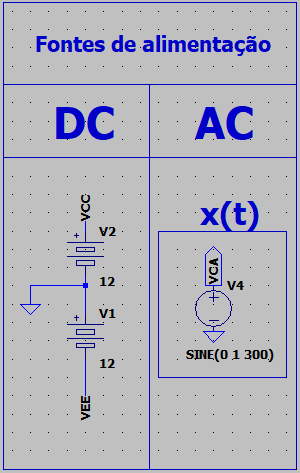
\includegraphics[scale = 0.6]{imagens/circuito/entrada.png}
\label{entrada_x}
\caption{Entrada $x(t)$ representada no LTSpice, com 1V de amplitue e f=300hz.}
\end{figure}

A entrada $x(t)$ do circuito foi modelada como uma fonte de sinal senoidal, representada por \textbf{V4}, e configurada para permitir a variação da frequência entre dierentes faixas, como 400 Hz - 450 Hz, e amplitude ajustável entre 1 V e 2 V. Essa configuração foi escolhida para representar um cenário realista de teste, permitindo analisar a resposta do circuito às variações de frequência e amplitude no domínio temporal. \\

A faixa de frequência foi projetada para atravessar os filtros ativos do sistema, possibilitando observar a precisão do filtro passa-baixa, passa-alta e passa-banda. A amplitude ajustável serve para avaliar a estabilidade e funcionalidade dos circuitos de detecção e comparação, garantindo que o sistema opere corretamente dentro dos limites especificados.


%%%%%%%%%%%%%%%%%%%%%%%%%%%%%%%%%%%%%%%%%%%%%%%%%%%%%%%%


\section{Resposta ao Impulso do Sistema $h(t)$}

O objetivo da análise da resposta ao impulso é avaliar o comportamento dinâmico do sistema em relação a estímulos instantâneos, como variações abruptas na entrada. Para o circuito em questão, a resposta ao impulso é utilizada como uma ferramenta para verificar a estabilidade, seletividade e precisão dos filtros implementados (passa-baixa, passa-alta e passa-banda), bem como para validar o desempenho dos circuitos de processamento de sinal.\\

Ao aplicar um impulso ao sistema, espera-se observar as características dos filtros projetados, como a atenuação fora das frequências de corte e a resposta ideal dentro da faixa de passagem. Esse tipo de análise também permite identificar possíveis ressonâncias, picos indesejados ou distorções que podem comprometer o desempenho do sistema como um todo.\\

Além disso, a análise da resposta ao impulso fornece informações importantes sobre o tempo de estabelecimento e o comportamento transiente do sistema, dados essenciais para garantir que o afinador de cordas responda de forma eficiente às frequências da entrada $x(t)$ e classifique corretamente o sinal para acionar a indicação correspondente.


\subsection{Filtro Passa-Baixa}

Um filtro passa-baixa é um dispositivo ou circuito eletrônico projetado para permitir a passagem de sinais com frequências mais baixas enquanto atenua ou bloqueia sinais com frequências mais altas. Ele é amplamente utilizado em sistemas de processamento de sinais, eletrônica e telecomunicações para diversas aplicações.\\

O filtro passa-baixa opera baseado no conceito de frequência de corte ($f_c$). Essa frequência define o limite entre as frequências que o filtro permite passar e aquelas que ele atenua. As principais características são:

\begin{enumerate}
    \item \textbf{Passagem de baixas frequências}: Sinais com frequências abaixo de $f_c$ passam pelo filtro com pouca ou nenhuma atenuação.
    \item \textbf{Atenuação de altas frequências}: Sinais com frequências acima de $f_c$ são gradualmente reduzidos em amplitude, dependendo da resposta do filtro.
\end{enumerate}

\subsubsection{Arquitetura Sallen-Key}

O filtro passa-baixa Sallen-key foi utilizado para captar frequências abaixo de 435Hz e, assim, acionar o LED amarelo. A equação padrão no domínio da frequência para um filtro passa-baixa de segunda ordem é dada por:

\begin{equation}
H_{LP} = \frac{K}{\left( -\left( \frac{f}{f_c} \right)^2 + j\frac{f}{Qf_c} + 1 \right)}
\end{equation}

Onde:
\begin{itemize}
    \item $f_c$ é a frequência de corte (notemos que $f_c$ é o ponto de transição entre a banda de passagem e a banda de rejeição, e não necessariamente a frequência de $-3$ dB);
    \item $Q$ é o fator de qualidade.
\end{itemize}

As características do filtro variam conforme a frequência:

\begin{itemize}
    \item Para $f \ll f_c$, a equação se reduz a $K$, e o circuito passa sinais multiplicados por um fator de ganho $K$.
    \item Quando $f = f_c$, a equação se reduz a $-jQ$, e os sinais são amplificados pelo fator $Q$.
    \item Para $f \gg f_c$, a equação se reduz a $-\frac{Kf_c^2}{f^2}$, e os sinais são atenuados pelo quadrado da razão da frequência. Essa atenuação em altas frequências aumenta com uma potência de 2, descrevendo a resposta do filtro passa-baixa de segunda ordem.
\end{itemize}

A Figura abaixo mostra o circuito Sallen-Key configurado como um passa-baixa:

\begin{figure}[H]
\centering
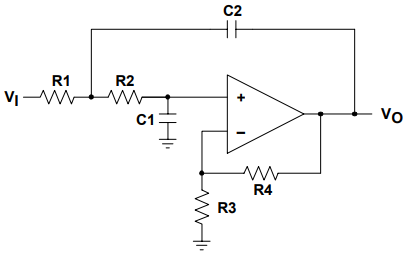
\includegraphics[scale=0.8]{imagens/circuito/filtro_passa-baixa_sallenKey.png}
\caption{Circuito Passa-Baixa Sallen-Key.}
\end{figure}

Para o circuito mostrado, as impedâncias e parâmetros são definidos como:

\begin{align}
Z_1 &= R_1, \quad Z_2 = R_2, \quad Z_3 = \frac{1}{sC_1}, \\
Z_4 &= \frac{1}{sC_2}, \quad K = 1 + \frac{R_4}{R_3}.
\end{align}

A função de transferência ideal do circuito Sallen-Key passa-baixa é expressa por:

\begin{equation}
H(s) = \frac{V_o}{V_i} (s) = \frac{K}{s^2 (R_1 R_2 C_1 C_2) + s \left( R_1 C_1 + R_2 C_1 + R_1 C_2 (1 - K) \right) + 1}
\end{equation}

Para simplificar a análise, consideremos as seguintes definições:
\begin{align}
s &= j2\pi f, \\
f_c &= \frac{1}{2\pi \sqrt{R_1 R_2 C_1 C_2}}, \\
Q &= \sqrt{\frac{R_1 R_2 C_1 C_2}{R_1 C_1 + R_2 C_1 + R_1 C_2 (1 - K)}}.
\end{align}

Com essas simplificações, a equação da função de transferência pode ser manipulada eficientemente para análise do filtro, usando métodos comumente aplicados em circuitos de segunda ordem.\\

O filtro Sallen-Key pode ser projetado de várias maneiras para atender às necessidades específicas de frequência de corte (\(f_c\)) e fator de qualidade (\(Q\)). Para simplificar o processo de design e facilitar a seleção de componentes, algumas simplificações são comumente aplicadas. Abaixo, são descritas quatro simplificações e os motivos para a escolha da primeira simplificação no projeto.\\

\textbf{Simplificação 1: Configuração dos Componentes como Razões}\label{ref:simp_1}\\

Nesta abordagem, considera-se \(R_1 = mR\), \(R_2 = R\), \(C_1 = C\) e \(C_2 = nC\), resultando nas equações:

\begin{equation}\label{fc_sim1}
    f_c = \frac{1}{2\pi RC\sqrt{mn}}    
\end{equation}

\begin{equation}\label{ref:fator_qualidade_fpb}
    Q = \frac{\sqrt{mn}}{m + 1 + mn(1 - K)}    
\end{equation}

Nesta configuração, os valores \(m\) e \(n\) determinam a relação entre os componentes, enquanto \(K\) representa o ganho no circuito. A interação entre os parâmetros \(f_c\), \(Q\) e \(K\) requer um design cuidadoso, começando pela escolha de \(m\), \(n\) e \(K\). Em situações práticas, \(K\) deve ser configurado para valores baixos para evitar oscilações indesejadas.\\

\textbf{Simplificação 2: Componentes como Razões com Ganho \(K = 1\)}\\

Aqui, considera-se \(R_1 = mR\), \(R_2 = R\), \(C_1 = C\) e \(C_2 = nC\), com o ganho \(K = 1\). As equações tornam-se:
\[
f_c = \frac{1}{2\pi RC\sqrt{mn}}
\]
\[
Q = \frac{\sqrt{mn}}{m + 1}
\]
A escolha de \(K = 1\) simplifica o projeto, mantendo o ganho unitário na banda de passagem. Porém, ainda há interação entre \(f_c\) e \(Q\), exigindo que \(m\) e \(n\) sejam cuidadosamente escolhidos.\\

\textbf{Simplificação 3: Resistores como Razões e Capacitores Iguais}\\

Nesta abordagem, \(R_1 = mR\), \(R_2 = R\) e \(C_1 = C_2 = C\). As equações tornam-se:
\[
f_c = \frac{1}{2\pi RC\sqrt{m}}
\]
\[
Q = \frac{\sqrt{m}}{1 + 2m - mK}
\]
Configurar os capacitores com valores iguais simplifica a seleção, mas limita as opções de projeto. O design ainda exige cuidado na escolha de \(m\) e \(K\) para evitar valores altos de \(Q\) que podem causar instabilidade.\\

\textbf{Simplificação 4: Componentes Iguais}\\

Considerando \(R_1 = R_2 = R\) e \(C_1 = C_2 = C\), as equações tornam-se:
\[
f_c = \frac{1}{2\pi RC}
\]
\[
Q = \frac{1}{3 - K}
\]
Essa simplificação elimina a interação entre \(f_c\) e \(Q\), simplificando o design. No entanto, como \(K\) controla \(Q\), ajustes adicionais podem ser necessários para atingir valores de ganho ou fator de qualidade desejados.\\

\textbf{Justificativa da Escolha da Simplificação 1}\\

A \textbf{Simplificação 1} foi escolhida devido à sua flexibilidade no ajuste de \(Q\) e \(f_c\). Essa abordagem permite o controle preciso da relação entre os componentes por meio dos parâmetros \(m\) e \(n\), sem impor restrições de igualdade entre resistores ou capacitores. Isso facilita a adaptação às especificações do projeto com componentes comerciais disponíveis, tornando o design mais eficiente e ajustável.\\





\subsubsection{Projetando o Filtro Passa-Baixa Sallen-key}
Com base na escolha feita, devemos realizar os cálculos necessários para a definição dos valores dos componentes do circuito em questão.\\

De acordo com a simplificação q, descrita em \ref{ref:simp_1}, vamos primeiro determinar os valores de $K$, $m$, $n$ e $Q$. Como nós estamos trabalhando com faixas de frequências muito estreitas, optamos por considerar um ganho $K$ em torno de $1.5$ e um fator de qualidade $Q$ em torno de $1$. Então, para tornar mais simples o processo de definição, fixamos $m=1$ e teremos, a partir da equação \ref{ref:fator_qualidade_fpb}:

\begin{equation}
    Q = 1 = \frac{\sqrt{n}}{2-n0.5}
\end{equation}


Resolvendo a equação, enontramos 

\[
n=1.53...
\]

Portanto, com $m=1$ e $n=1.53$, podemos definir os valores dos componentes com base na simplificação 1 descrita em \ref{ref:simp_1}.\\ 

Escolhendo $C_1 = 10n$, teremos:


\begin{equation*}
    C_2 = C_1*n = 1.53 * 10 * 10^{-9} = 15.3*10^{-9}
\end{equation*}

E também, , da equação \ref{fc_sim1}:

\begin{equation}
    f_c = 435hz = \frac{1}{2\pi R_2 10 *10^{-9} \sqrt{1.53} }

\end{equation}


O que resultou em 

\begin{equation*}
    R_2 \approx 29.0
\end{equation*}

Logo, como $R_1 = mR_2$

\begin{equation*}
    R_1 = R_2 = 29k \Omega
\end{equation*}

Então, após alguns ajustes manuais até alcançarmos um estado ótimo do filtro, definimos os valores dos componentes, representados na imagem seguinte:

\begin{figure}[H]
\centering
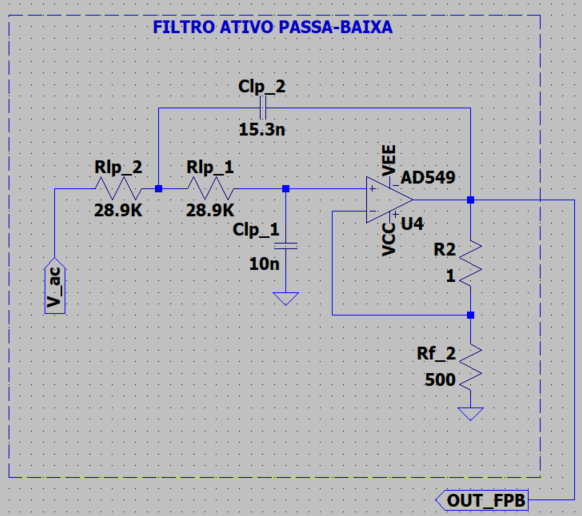
\includegraphics[scale=0.8]{imagens/circuito/filtro_passa-baixa_LTSpice.png
}
\caption{Filtro Passa-Baixa Sallen-Key projetado no LTSpice}
\end{figure}


\subsubsection{Simulação AC Sweep}

Após a projeção do filtro, fizemos a simulação AC a partir da saída \texttt{OUT\_FPB}. Na imagem seguinte, podemos verificar, ao fixar o cursor próximo da frequência de corte, que o filtro começa a deixar as altas frequências (i.e., acima de 435hz) passarem, atenunando com mais veemência as frequências abaixo deste valor.

\begin{figure}[H]
\centering
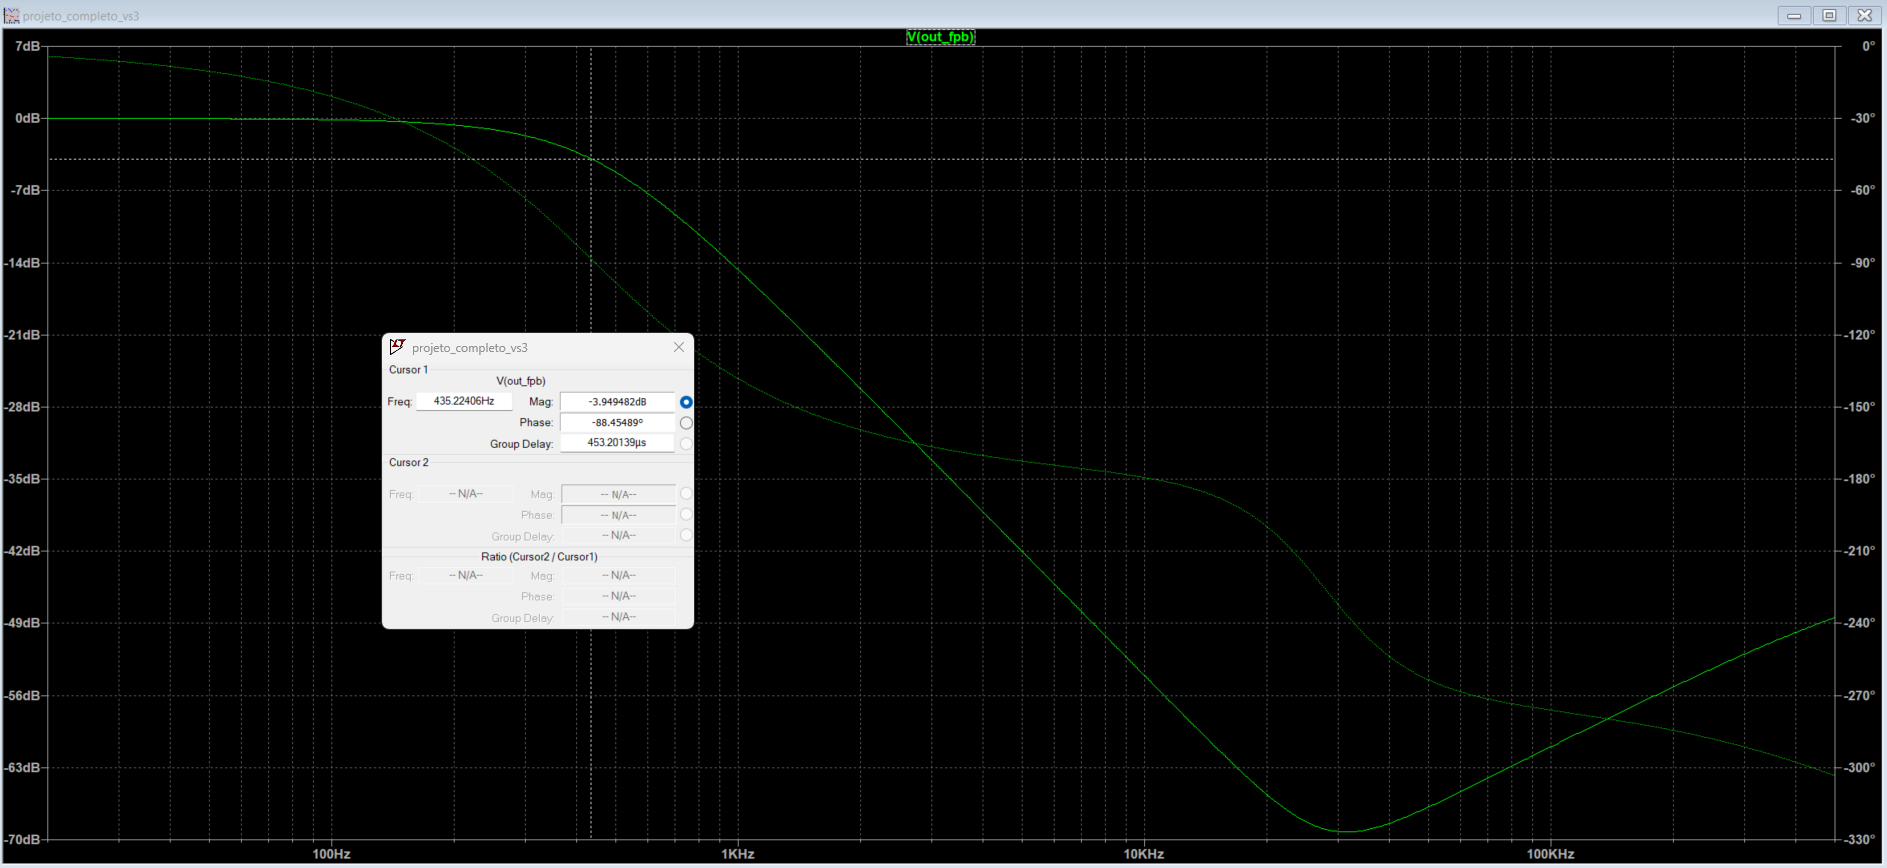
\includegraphics[scale=0.4]{imagens/graficos/ac_sweep_passa-baixa.png}

\caption{Simulação AC Sweep do Filtro Passa-Baixa Sallen-Key}
\end{figure}

\subsection{Filtro Passa-Alta}

Um filtro passa-alta é um circuito projetado para permitir a passagem de sinais com frequências acima de uma frequência de corte específica ($f_c$), enquanto atenua sinais com frequências mais baixas. Ele é amplamente utilizado em sistemas de comunicação, eletrônica e processamento de sinais.\\

O filtro passa-alta Sallen-Key utilizado no projeto segue uma arquitetura similar à do passa-baixa, com as seguintes diferenças principais:

\begin{itemize}
    \item No passa-alta, os capacitores assumem o papel de componentes de entrada e os resistores definem a resposta de frequência do circuito. Isso é inverso ao passa-baixa, onde os resistores estão na entrada e os capacitores determinam a atenuação em altas frequências.
    \item A função de transferência apresenta um comportamento que amplifica sinais para $f \gg f_c$ e atenua sinais abaixo de $f_c$, ao contrário do passa-baixa.
\end{itemize}

A equação padrão no domínio da frequência para o passa-alta de segunda ordem é expressa por:

\begin{equation}
H_{HP} = \frac{-K\left(\frac{f}{f_c}\right)^2}{1 - \left(\frac{f}{f_c}\right)^2 + j\frac{f}{Qf_c}}
\end{equation}

Assim como no passa-baixa, as frequências críticas são definidas pelo ponto de corte $f_c$ e pelo fator de qualidade $Q$:

\begin{itemize}
    \item Para $f \ll f_c$, a função se reduz a uma atenuação proporcional ao quadrado da frequência.
    \item Para $f = f_c$, a função se reduz a $-jQ$, e os sinais são amplificados pelo fator $Q$.
    \item Para $f \gg f_c$, a função converge para $K$, e o circuito permite a passagem do sinal multiplicado pelo ganho $K$.
\end{itemize}

A arquitetura do passa-alta Sallen-Key, apresentada na figura abaixo, é baseada em capacitores na entrada e resistores como elementos de feedback:

\begin{figure}[H]
\centering
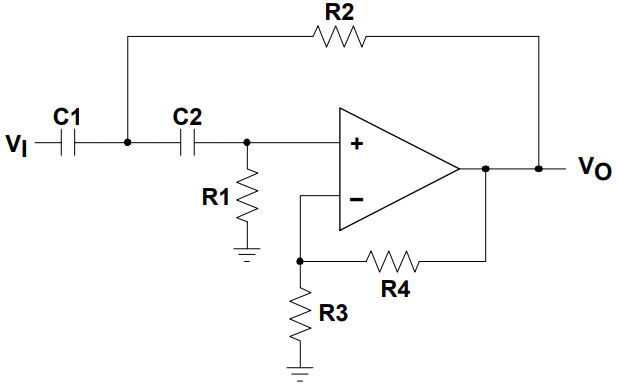
\includegraphics[scale=0.6]{imagens/circuito/filtro_passa-alta_sallenKey.png}
\caption{Circuito Passa-Alta Sallen-Key.}
\end{figure}

Para o circuito mostrado, as impedâncias e parâmetros são definidos como:

\begin{align}
Z_1 &= \frac{1}{sC_1}, \quad Z_2 = \frac{1}{sC_2}, \quad Z_3 = R_1, \quad Z_4 = R_2, \quad K = 1 + \frac{R_4}{R_3}.
\end{align}

A função de transferência ideal é dada por:

\begin{equation}
H(s) = \frac{V_o}{V_i} (s) = \frac{-Ks^2 (R_1 R_2 C_1 C_2)}{s^2 (R_1 R_2 C_1 C_2) + s \left( R_2 C_1 + R_1 C_1 + R_1 C_2 (1 - K) \right) + 1}
\end{equation}

Os parâmetros de corte e qualidade podem ser calculados conforme as seguintes definições:

\begin{align}
f_c &= \frac{1}{2\pi \sqrt{R_1 R_2 C_1 C_2}}, \\\\
Q &= \sqrt{\frac{R_1 R_2 C_1 C_2}{R_2 C_1 + R_1 C_1 + R_1 C_2 (1 - K)}}.
\end{align}

\subsubsection{Projetando o Filtro Passa-Alta Sallen-key}

\textbf{Simplificação Utilizada:}\\
Para o projeto do passa-alta, utilizamos a \textbf{Simplificação 1}, descrita anteriormente para o passa-baixa, que consiste em:

\[
    R_1 &= mR, \quad R_2 = R, \quad C_1 = C, \quad C_2 = nC 
\]

Onde $m=1$ e $n=1.53$, como definimos anteriormente. Então temos, consequentemente, que $C_2 = 15.3nF$ ao fixarmos $C_1 = 10nF$.\\

Com essa configuração, foi possível definir os componentes do circuito, priorizando o ajuste preciso da frequência de corte superior ($f_c = 445$ Hz) e o fator de qualidade ($Q \approx 1$), garantindo uma resposta adequada na faixa de frequências desejada.

\begin{equation*}
    f_c = 445hz = \frac{1}{2\pi R_2 10 *10^{-9} \sqrt{1.53} } \longrightarrow R_2 = R_1 = 29.6 k\Omega
\end{equation*}



\begin{figure}[H]
\centering
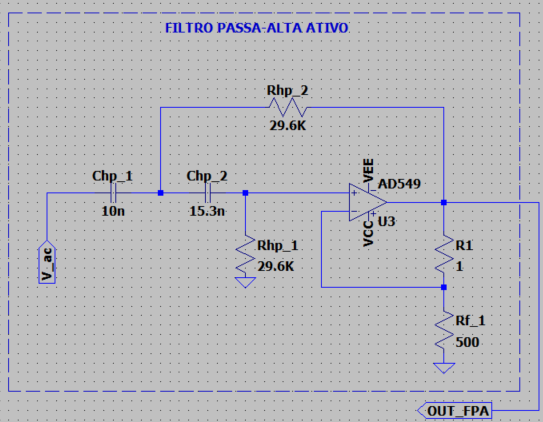
\includegraphics[scale=0.85]{imagens/circuito/filtro_passa-alta_LTSpice.png}
\caption{Filtro Passa-Alta Sallen-Key projetado no LTSpice.}
\end{figure}

\subsubsection{Simulação AC Sweep}

Abaixo, a simulação do filtro realizada no LTSpice. Ao fixarmos o cursor em, aproximadamente, 445hz, que é a frequência de corte, podemos observar que o filtro começa a estabilizar a passagem das frequências acima deste valor.

\begin{figure}[H]
\centering
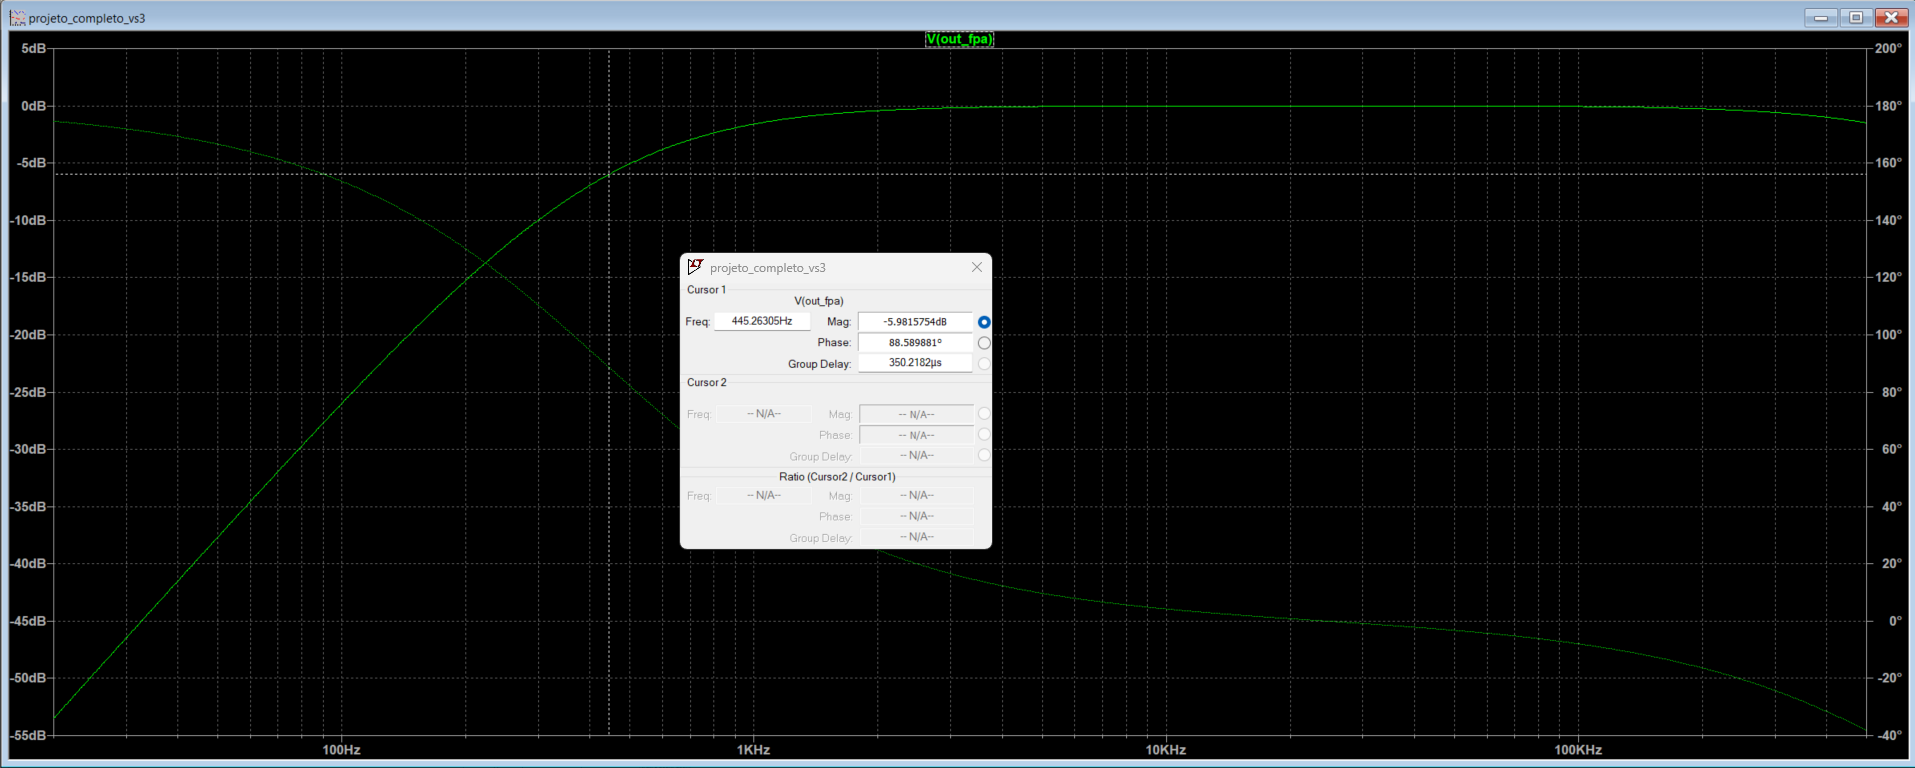
\includegraphics[scale=0.3]{imagens/graficos/ac_sweep_passa-alta.png}
\caption{Simulação AC do filtro Passa-Alta no LTSpice.}
\end{figure}


\subsection{Filtro Passa-Banda}

O filtro Passa-Banda consiste em um filtro que permite a passagem de frequências que estão entre as baixas e altas. Seu \textit{design} consiste na junção de ambos os filtros Passa-Baixa e Passa-Alta anteriormente projetados, tendo como propriedade ser obrigatoriamente de segunda ordem. No projeto foi escolhido para detectar as frequências entre 435Hz e 445Hz, acendendo, dessa forma, o LED verde.

Suas características são:

\begin{itemize}
    \item \textbf{Passagem de frequências medianas:} sinais entre as frequências de corte da parte consistente do filtro Passa-Baixa e Passa-Alta sofrem pouca ou nenhuma alteração.
    \item \textbf{Atenuação de frequências baixas e altas:} sinais que se distanciam tanto para baixo quanto para cima a partir de, respectivamente, $f_c$ do Passa-Baixa e $f_c$ do Passa-Alta são bloqueados. 
 \end{itemize}


\subsubsection{Arquitetura Sallen-Key}

A partir do projeto dos filtros anteriores a modelagem consiste na passagem da tensão primeiramente pelo Passa-Baixa e depois pelo Passa-Alta, assim possuindo o $V_{out}$ esperado para o filtro Passa-Banda. 

\begin{figure}[H]
\centering
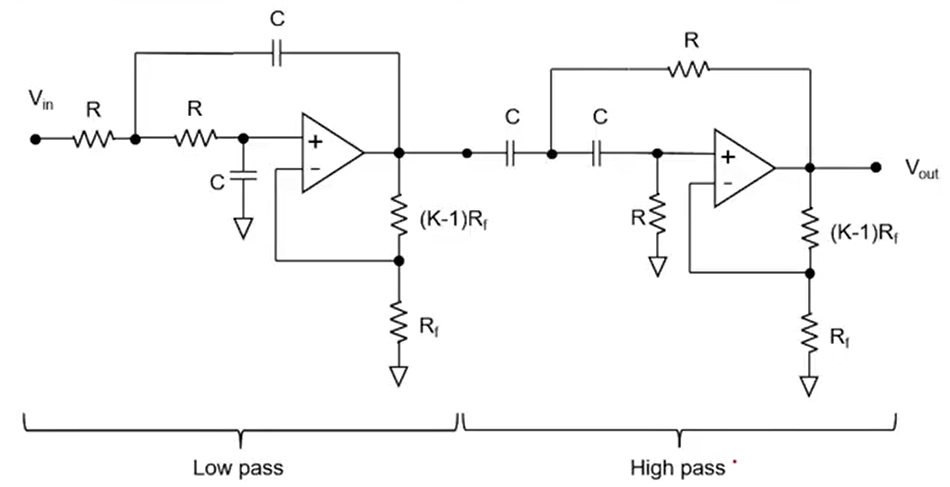
\includegraphics[scale=0.6]{imagens/circuito/bandpass_sallen-key.png}
\caption{Circuito Passa-Banda - Topologia Sallen-Key}
\end{figure}

\subsubsection{Projetando o Filtro Passa-Banda Sallen-key}
O filtro projetado é do tipo Sallen-Key de segunda ordem, pois cada estágio (passa-baixa e passa-alta) usa dois elementos reativos (capacitores) e dois resistores, o que caracteriza um filtro de segunda ordem. A combinação dos dois estágios resulta em um filtro passa-banda de quarta ordem no total.

\subsubsection*{Cálculo das Frequências de Corte}

As frequências de corte superior ($f_h$) e inferior ($f_l$) de um filtro passa-banda podem ser calculadas usando a fórmula para circuitos Sallen-Key:

\begin{equation}
    f_c = \frac{1}{2 \pi \sqrt{R_1 R_2 C_1 C_2}}
\end{equation}

\noindent Onde:
\begin{itemize}
    \item $R_1, R_2$: Resistores da rede Sallen-Key;
    \item $C_1, C_2$: Capacitores da rede Sallen-Key.
\end{itemize}

\noindent Para o circuito projetado, os valores de resistores e capacitores são os seguintes:

\begin{itemize}
    \item \textbf{Filtro Passa-Baixa:}
    \begin{itemize}
        \item $R_{bp3} = R_{bp4} = 28.9k\ \Omega$
        \item $C_{bp3} = 15.3\ \mathrm{nF}$
        \item $C_{bp4} = 10\ \mathrm{nF}$
    \end{itemize}
    
    \item \textbf{Filtro Passa-Alta:}
    \begin{itemize}
        \item $R_{hp1} = R_{hp2} = 29.6k\ \Omega$
        \item $C_{hp1} = 15.3\ \mathrm{nF}$
        \item $C_{hp2} = 10\ \mathrm{nF}$
    \end{itemize}
\end{itemize}

\begin{figure}[H]
\centering
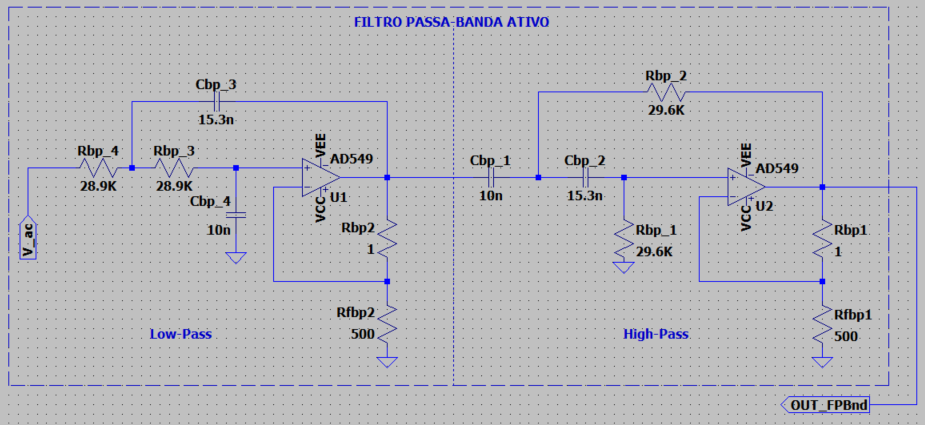
\includegraphics[scale=0.7]{imagens/circuito/filtro_passa-banda_LTSpice.png}
\caption{Filtro Passa-Banda projetado no LTSpice}
\end{figure}

\paragraph{1. Frequência de Corte Inferior ($f_l$):}

A frequência de corte inferior do filtro passa-baixa é calculada como:

\begin{equation}
    f_l = \frac{1}{2 \pi \sqrt{R_{bp3} R_{bp4} C_{bp3} C_{bp4}}}
\end{equation}

\noindent Substituindo os valores:

\begin{equation*}
    f_l = \frac{1}{2 \pi \sqrt{(28.9 \times 10^3)(28.9 \times 10^3)(15.3 \times 10^{-9})(10 \times 10^{-9})}}
\end{equation*}

\begin{equation*}
    f_l \approx 434.6 hz
\end{equation*}

\paragraph{2. Frequência de Corte Superior ($f_h$):}

A frequência de corte superior do filtro passa-alta é calculada como:

\begin{equation}
    f_h = \frac{1}{2 \pi \sqrt{R_{hp1} R_{hp2} C_{hp1} C_{hp2}}}
\end{equation}

\noindent Substituindo os valores:

\begin{equation}
    f_h = \frac{1}{2 \pi \sqrt{(29.6 \times 10^3)(29.6 \times 10^3)(15.3 \times 10^{-9})(10 \times 10^{-9})}}
\end{equation}

\begin{equation*}
    f_h \approx 445.5 hz
\end{equation*}

Com base nos valores calculados, essas frequências determinam as bordas do intervalo de operação do filtro passa-banda, garantindo que apenas sinais dentro dessa faixa sejam processados pelo sistema. Esses valores foram escolhidos para atender às especificações de corte em 435 Hz (passa-baixa) e 445 Hz (passa-alta).


\subsubsection{Simulação AC Sweep}

Ao fixarmos o cursor, podemos verificar que a frequência central, de fato, está  identificada em torno de $440hz$, como esperado.

\begin{figure}[H]
\centering
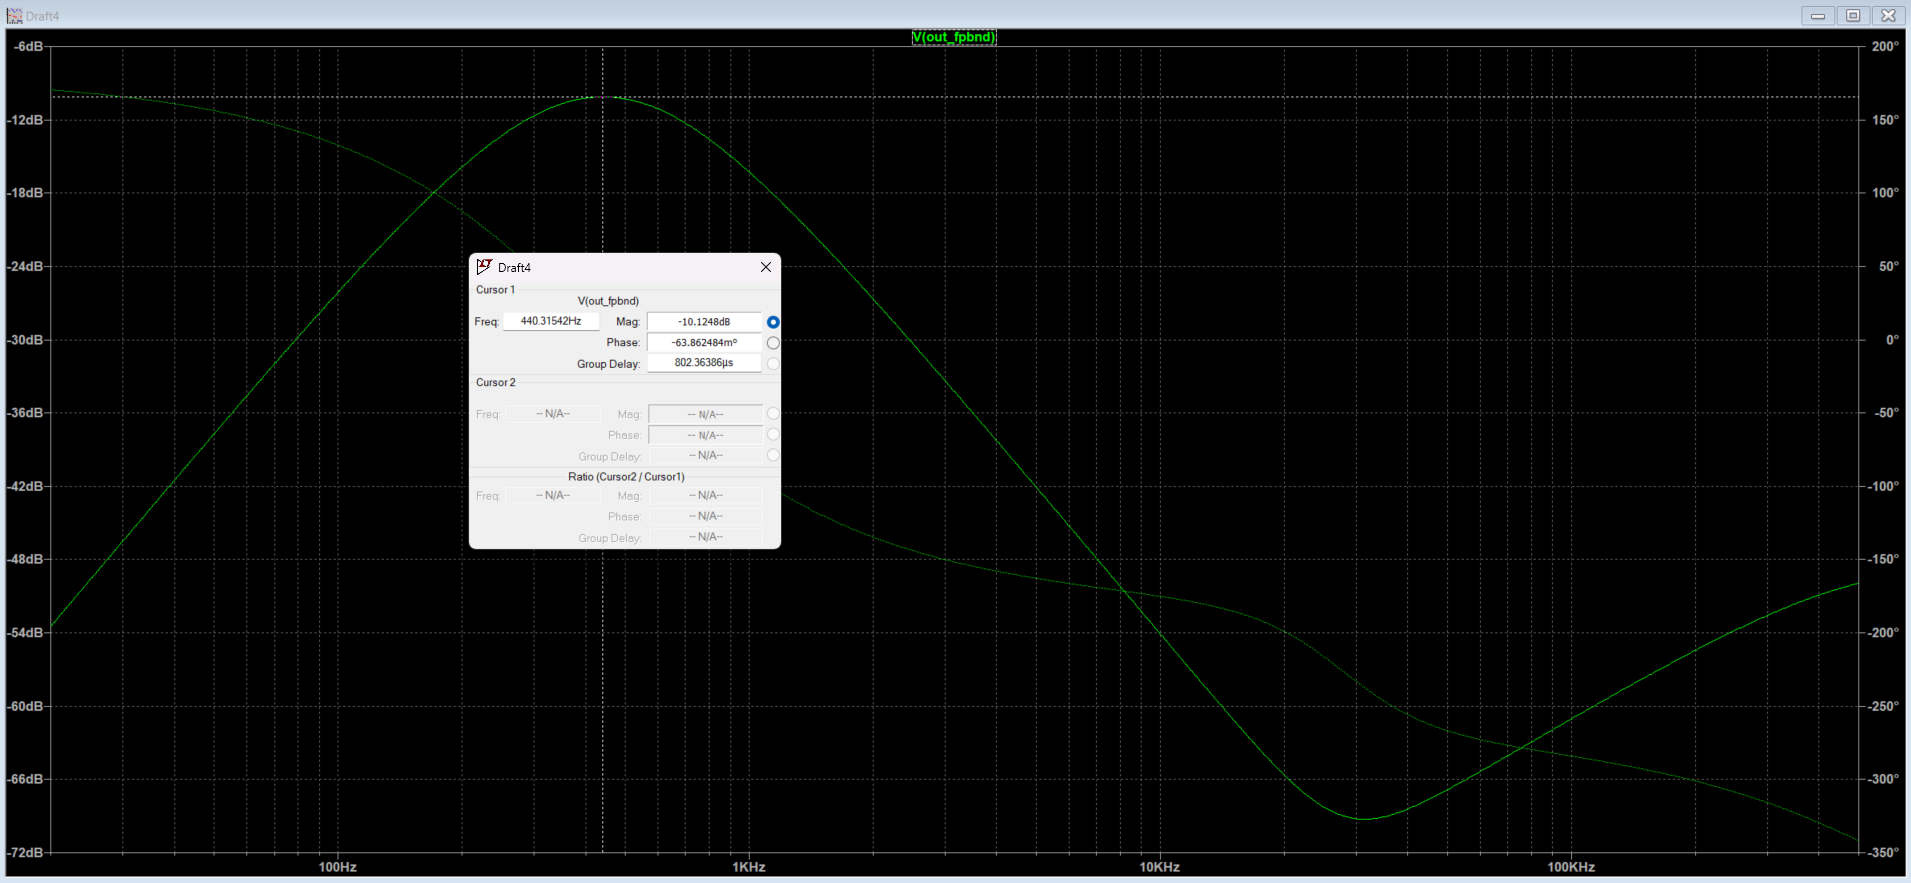
\includegraphics[scale=0.3]{imagens/graficos/passa-banda_acsweep.png}
\caption{Simulação AC para o filtro passa-banda}
\end{figure}


%%%%%%%%%%%%%%%%%%%%%%%%%%%%%%%%%%%%%%%%%%%%%%%%%%%%%

\section{Saída $y(t)$}

A saída \( y(t) \) do circuito representa a informação processada e extraída do sinal de entrada \( x(t) \) após ser tratado pelos filtros \( h(t) \). Nesta seção, explicaremos o funcionamento e as implementações dos estágios responsáveis pelo processamento, detecção e indicação, detalhando como cada componente contribui para o comportamento geral do sistema.

\subsection{Processamento e Extração de Informações do Sinal}

\subsubsection{Buffer}

O Buffer é um estágio fundamental no circuito que garante a integridade do sinal ao longo do processamento. Ele é configurado como um amplificador de ganho unitário (\( \text{ganho} = 1 \)) e possui as seguintes características:

\begin{itemize}
    \item \textbf{Alta impedância de entrada:} Reduz o impacto do estágio subsequente sobre o estágio anterior, minimizando distorções.
    \item \textbf{Baixa impedância de saída:} Assegura que o estágio subsequente receba corrente suficiente sem degradação do sinal.
    \item \textbf{Isolamento elétrico:} Protege os estágios anteriores de variações no estágio subsequente.
\end{itemize}

\paragraph{Implementação Típica:} O Buffer é implementado com um amplificador operacional em configuração de seguidor de tensão, onde a saída do AmpOp é conectada à entrada inversora, e a entrada não inversora recebe o sinal.

\begin{figure}[H]
\centering
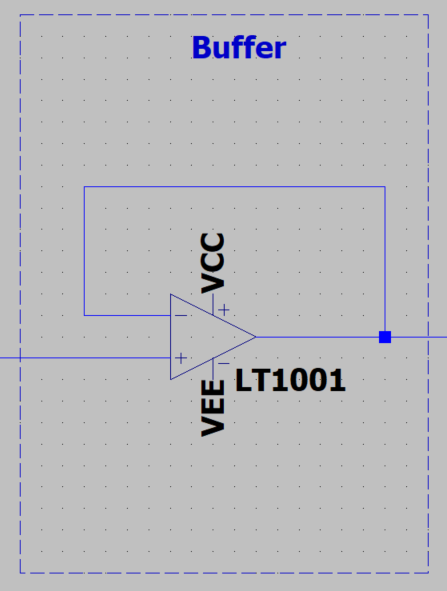
\includegraphics[scale=0.8]{imagens/circuito/buffer.png}
\caption{Buffer projetado no LTSpice}
\end{figure}


\subsubsection{Circuito Detector de Pico}

O circuito detector de pico é responsável por capturar e reter o valor de pico do sinal senoidal de entrada, essencial para que os comparadores de tensão funcionem corretamente. Ele fornece uma referência estável, baseada na amplitude máxima do sinal, para determinar a faixa de frequência correspondente.

\subsubsection*{Configuração Geral} 
O detector de pico é composto por:
\begin{itemize}
    \item \textbf{Amplificador operacional:} Configurado como seguidor de tensão, evita que o circuito detector interfira na fonte do sinal.
    \item \textbf{Diodo:} Permite a passagem de corrente na direção positiva, armazenando o valor de pico.
    \item \textbf{Capacitor:} Armazena a tensão máxima detectada no sinal.
    \item \textbf{Resistor paralelo:} Proporciona um caminho de descarga lento para o capacitor, garantindo resposta a alterações no sinal.
\end{itemize}

\paragraph{Funcionamento}
\begin{itemize}
    \item \textbf{Entrada do Sinal:} O circuito recebe um sinal senoidal com amplitude determinada.
    \item \textbf{Retificação pelo Diodo:} Durante o ciclo positivo do sinal, o diodo conduz e permite que a tensão de pico seja capturada. Durante o ciclo descendente, o diodo bloqueia a descarga do capacitor.
    \item \textbf{Armazenamento pelo Capacitor:} O capacitor retém a tensão de pico até que um valor superior seja detectado. O resistor paralelo permite uma descarga controlada, garantindo resposta lenta a alterações.
    \item \textbf{Isolamento pelo Amplificador Operacional:} Um seguidor de tensão isola o circuito de detecção do restante do sistema, mantendo a tensão armazenada no capacitor estável.
\end{itemize}

\begin{figure}[H]
\centering
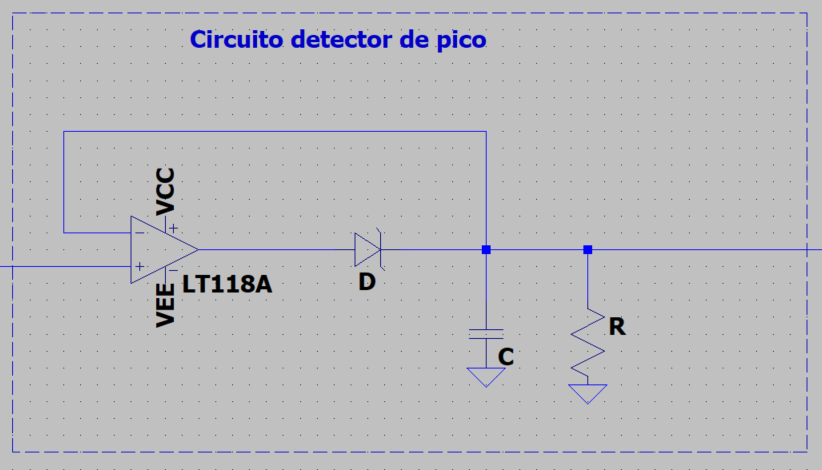
\includegraphics[scale=0.7]{imagens/circuito/detector_de_pico_LTSpice.png}
\caption{Detector de Pico projetado no LTSpice}
\end{figure}




\subsubsection{Circuito de Comparação}

Os comparadores determinam qual LED será acionado com base na frequência detectada pelo circuito. Cada comparador é configurado para operar em uma faixa específica, associada a um LED:

\begin{itemize}
    \item \textbf{Filtro passa-baixa (\(< 435 \, \text{Hz}\)):} Aciona o LED amarelo.
    \item \textbf{Filtro passa-banda (\(435 \, \text{Hz} \leq f \leq 445 \, \text{Hz}\)):} Aciona o LED verde.
    \item \textbf{Filtro passa-alta (\(> 445 \, \text{Hz}\)):} Aciona o LED vermelho.
\end{itemize}

\paragraph{Operação dos Comparadores}
Cada comparador recebe:
\begin{itemize}
    \item A saída do filtro correspondente na entrada não inversora (\( V_+ \)).
    \item A tensão de referência dinâmica, calculada a partir do detector de pico, na entrada inversora (\( V_- \)).
\end{itemize}
Se \( V_+ > V_- \), o comparador gera uma saída alta, polarizando o transistor correspondente e acionando o LED.

\begin{figure}[H]
\centering
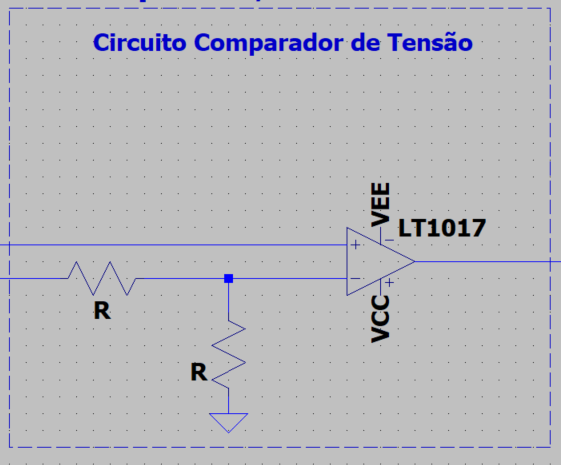
\includegraphics[scale=0.8]{imagens/circuito/comparador_tensao.png}
\caption{Circuito Comparador de Tensão projetado no LTSpice}
\end{figure}




\subsection{Indicação}

\subsubsection{Transistor NPN}
O transistor NPN é usado como um interruptor para controlar o acionamento dos LEDs. Ele funciona da seguinte forma:
\begin{itemize}
    \item \textbf{Base (B):} Um pequeno sinal de corrente aqui determina se o transistor está em corte (desligado) ou saturação (ligado).
    \item \textbf{Coletor (C):} Permite a passagem de corrente para o LED quando o transistor é acionado.
    \item \textbf{Emissor (E):} O terminal por onde a corrente sai.
\end{itemize}

\paragraph{Modo de Operação}
Quando o comparador associado a uma faixa de frequência ativa sua saída, ele polariza a base do transistor correspondente. Isso permite que a corrente flua do coletor para o emissor, acionando o LED apropriado.

\begin{figure}[H]
\centering
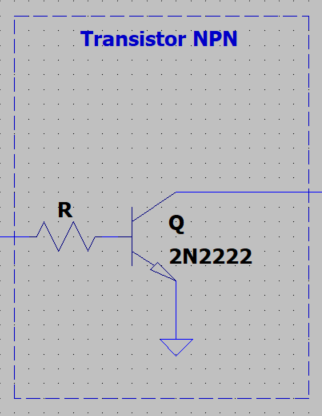
\includegraphics[scale=0.8]{imagens/circuito/transistor_NPN.png}
\caption{Transistor NPN projetado no LTSpice}
\end{figure}



\subsubsection{LED Drivers}
O LED driver controla a corrente que passa por cada LED, garantindo sua operação eficiente e segura. Cada LED é conectado em série com:
\begin{itemize}
    \item Um resistor limitador de corrente.
    \item O coletor de um transistor NPN.
\end{itemize}

\paragraph{Funcionamento}
Quando um comparador detecta uma frequência correspondente à sua faixa, ele envia um sinal alto ao transistor associado, permitindo que o LED acenda. Os demais LEDs permanecem apagados, pois seus transistores estão no estado de corte.

\begin{figure}[H]
\centering
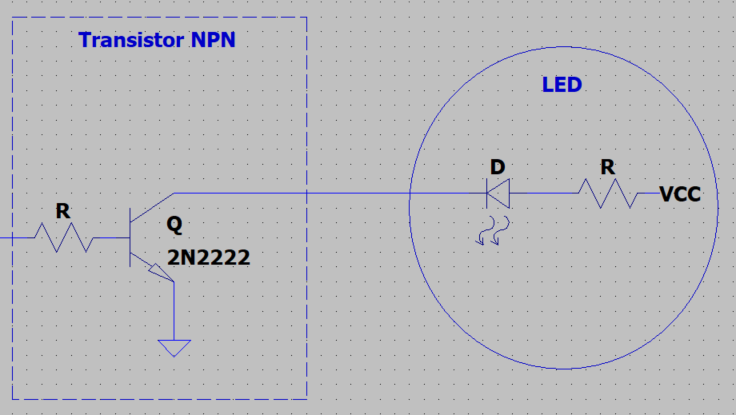
\includegraphics[scale=0.8]{imagens/circuito/led_driver.png}
\caption{LED Driver projetado no LTSpice}
\end{figure}



%%%%%%%%%%%%%%%%%%%%%%%%%%%%%%%%%%%%%%%%%%%%%%%%%%%%%%%%
\section{Montagem e Simulação no LTSpice}

A montagem do circuito completo no LTSpice foi realizada com base nos blocos funcionais definidos para o sistema, que processam o sinal de entrada $x(t)$, aplicam as funções de transferência 
$h(t)$, e geram o sinal de saída 
$y(t)$. Cada bloco foi implementado e configurado com componentes ajustados para garantir o funcionamento conforme os requisitos especificados.

\subsection{Sinal de Entrada}
O sinal de entrada $x(t)$  foi modelado como uma fonte de tensão alternada (\texttt{SINE}) variando em amplitude e frequência. Esse sinal representa as frequências de teste que foram aplicadas ao sistema. Adicionalmente, fontes de alimentação DC foram configuradas para fornecer a polarização correta aos amplificadores operacionais e transistores utilizados.

\subsubsection{Fonte Senoidal }

A fonte senoidal foi configurada para gerar para gerar uma senoide de amplitude variada (1V-2V) e frequência ajustável.

\begin{figure}[H]
\centering
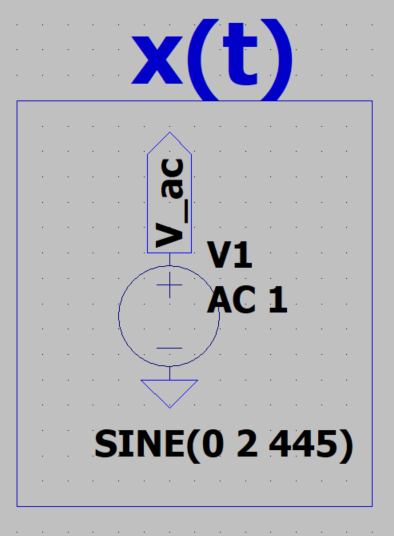
\includegraphics[scale=0.5]{imagens/circuito/fonte_xt.png}
\caption{Fonte senoidal projetada no LTSpice}
\end{figure}

\subsubsection{Fontes DC +12V e -12V}
As fontes DC fornecem $+12V$ e $-12V$, garantindo a operação adequada dos amplificadores operacionais do circuito.

\begin{figure}[H]
\centering
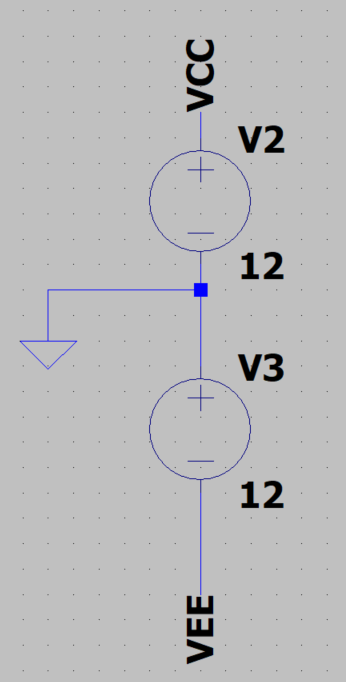
\includegraphics[scale=0.3]{imagens/circuito/fontes_dc.png}
\caption{Fontes DC projetadas no LTSpice}
\end{figure}


\subsection{Filtragem do Sinal de Entrada - Bloco $h(t)$}

A função $h(t)$ foi implementada por meio de blocos de filtragem ativa que processam o sinal de entrada $x(t)$, dividindo-o em diferentes faixas de frequência. O objetivo foi separar os componentes do sinal em três categorias: frequências abaixo de 435 Hz (passa-baixa), entre 435 Hz e 445 Hz (passa-banda), e acima de 445 Hz (passa-alta). Cada filtro foi ajustado para garantir precisão nas frequências de corte.

\begin{figure}[H]
\centering
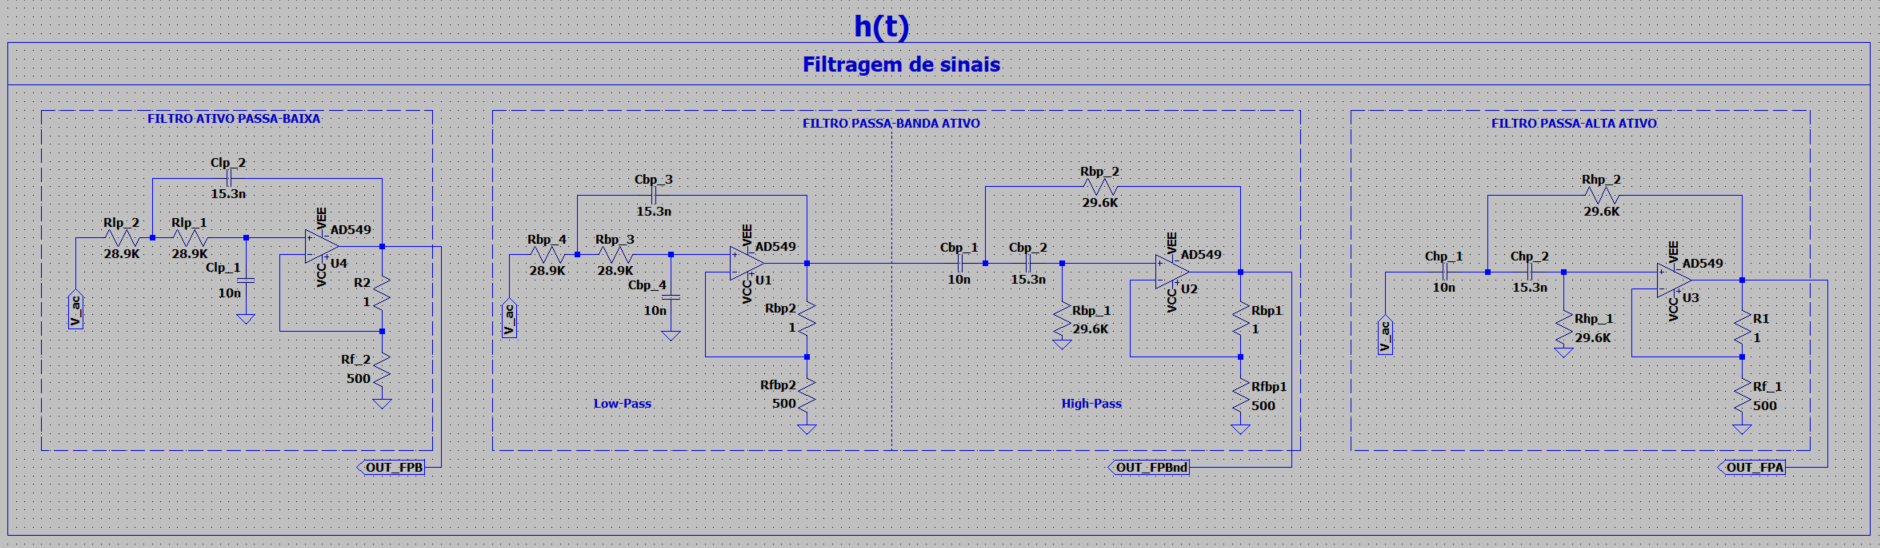
\includegraphics[scale=0.35]{imagens/circuito/filtragem_sinais.png}
\caption{Bloco h(t): filtragem de sinais no LTSpice}
\end{figure}


\subsection{Análise e Tratamento do Sinal - Saída $y(t)$}

Após a filtragem, o sinal de saída $y(t)$ passa por um estágio de detecção e tratamento, que inclui a identificação de picos de tensão e a comparação com valores de referência. Este processo é essencial para o funcionamento do sistema de indicação visual.

\subsubsection{Análise e Tratamento do Sinal da Fonte}

A figura abaixo apresenta o estágio de detecção de pico para o sinal de entrada gerado pela fonte (\( V_{ac} \)). Esse estágio tem como objetivo capturar o valor máximo (pico) do sinal de entrada alternado para ser utilizado nos estágios subsequentes, como os comparadores de tensão.


\begin{figure}[H]
\centering
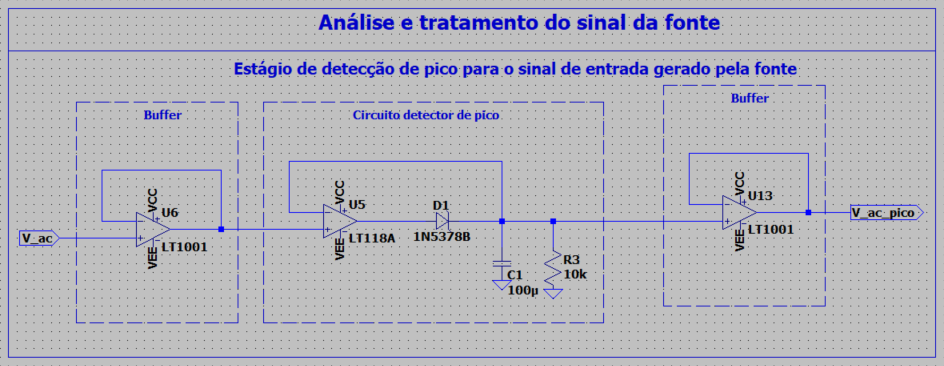
\includegraphics[scale=0.6]{imagens/circuito/analise_sinais_da_fonte.png}
\caption{Tratamento do sinal da fonte senoidal}
\end{figure}

\paragraph{Buffer de Entrada (U6):}
O amplificador operacional \( U6 \) está configurado como um buffer (seguidor de tensão). Sua função é isolar a fonte \( V_{ac} \) e fornecer um sinal de baixa impedância para o circuito subsequente. Com isso, garante-se que o sinal \( V_{ac} \) seja transmitido sem perda ou distorção.

\paragraph{Circuito Detector de Pico (U5, D1, C1, R3):}
Este bloco é responsável por capturar e armazenar o valor de pico do sinal \( V_{ac} \):
\begin{itemize}
    \item O amplificador operacional \( U5 \) amplifica o valor de pico do sinal de entrada.
    \item O diodo \( D1 \) (1N5378B) permite que apenas a corrente correspondente ao valor máximo do sinal flua para o capacitor \( C1 \).
    \item O capacitor \( C1 \) armazena o valor de pico, representando a amplitude máxima do sinal \( V_{ac} \).
    \item O resistor \( R3 \) proporciona um caminho de descarga lenta para \( C1 \), permitindo que o circuito acompanhe variações na amplitude do sinal ao longo do tempo.
\end{itemize}
O resultado desse bloco é o valor máximo \( V_{ac\_pico} \), que representa a amplitude do sinal alternado.

\paragraph{Buffer de Saída (U13):}
O amplificador operacional \( U13 \) está configurado como outro buffer. Ele isola o circuito detector de pico da próxima etapa do sistema, garantindo que \( V_{ac\_pico} \) seja transmitido sem alterações e com baixa impedância.\\

\paragraph{Relevância do Estágio:}
O circuito de detecção de pico é essencial para converter o sinal alternado em uma representação de sua amplitude máxima. O valor \( V_{ac\_pico} \) será utilizado como referência nos comparadores de tensão, permitindo que o sistema identifique a intensidade do sinal. Em conjunto com os outros blocos, esse estágio contribui para decidir qual LED será ativado, indicando a faixa de frequência e amplitude correspondente, levando em conta a tensão senoidal da fonte. Isso é importante, pois um sinal gerado pela fonte a 2V a uma determinada frequência, por exemplo, não terá o mesmo valor de amplitude que um sinal gerado pela mesma fonte a 1V com a mesma frequência.  \\
O uso de buffers na entrada e saída garante a integridade do sinal durante o processamento. Isso protege tanto a fonte de entrada quanto o estágio seguinte de qualquer interferência ou alteração no sinal, tornando o circuito confiável e preciso para o objetivo proposto.

\subsubsection{Projetando o Comparador Dinâmico}

O comparador dinâmico foi projetado para operar com referências proporcionais à amplitude detectada do sinal de entrada, garantindo funcionamento adequado para qualquer valor de amplitude entre $1\, \mathrm{V}$ e $2\, \mathrm{V}$. Isso elimina a necessidade de normalização ou regulação adicional do sinal de entrada, simplificando o projeto. Abaixo detalhamos o funcionamento:

\paragraph{Objetivo:}
O comparador deve operar de forma que:
\begin{itemize}
    \item A referência do comparador ($V_{\mathrm{ref}}$) seja proporcional ao pico da amplitude do sinal de entrada ($V_{\mathrm{pico}}$).
    \item O LED correspondente acenda corretamente para frequências específicas, independentemente da amplitude do sinal de entrada.
\end{itemize}

\paragraph{Etapas do Funcionamento:}
\begin{enumerate}
    \item \textbf{Detecção do Pico:} O circuito retificador de pico captura o valor máximo da tensão de entrada ($V_{\mathrm{pico}}$). Este estágio é implementado com diodos e capacitores que armazenam o pico do sinal.
    
    \item \textbf{Geração da Referência ($V_{\mathrm{ref}}$):} A tensão de referência dinâmica é gerada a partir de um divisor resistivo ajustável, proporcional ao valor de $V_{\mathrm{pico}}$. 
    Foram feitos alguns testes para verificar as amplitude de cada filtro ao ser alimentado pela fonte senoidal a diferentes valores de tensão, entre 1V e 2V. Os resultados foram os seguintes:
    
    \begin{itemize}
        \item \textbf{Para o filtro Passa-Baixa}:
        \begin{itemize}
            \item Quando $V_{in} = 1V$ e $f=435hz$, a amplitude do sinal na saída do filtro é $\approx 633mV$;
            \item Quando $V_{in} = 2V$ e $f=435hz$, a amplitude do sinal na saída do filtro é $\approx 1.27V$;
        \end{itemize}

        Com isso, concluímos que a tensão de pico do filtro passa-baixa fica em torno de 63\% do pico do sinal de entrada.\\

        \item \textbf{Para o filtro Passa-Alta}:
        \begin{itemize}
            \item Quando $V_{in} = 1V$ e $f=445hz$, a amplitude do sinal na saída do filtro é $\approx 502mV$;
            \item Quando $V_{in} = 2V$ e $f=445hz$, a amplitude do sinal na saída do filtro é $\approx 1V$;
        \end{itemize}

        Com isso, concluímos que a tensão de pico do filtro passa-baixa fica em torno de 50\% do pico do sinal de entrada.\\

    \item \textbf{Para o filtro Passa-Banda}:
        \begin{itemize}
            \item Quando $V_{in} = 1V$ e $445hz \leq f \leq 435hz$, a amplitude do sinal na saída do filtro é $\approx 311.5mV$;
            \item Quando $V_{in} = 2V$ e $445hz \leq f \leq 435hz$, a amplitude do sinal na saída do filtro é $\approx 622mV$;
        \end{itemize}

        Com isso, concluímos que a tensão de pico do filtro passa-baixa fica em torno de 31\% do pico do sinal de entrada.
    \end{itemize}
    
    Então, a proporção é definida por um fator $k$, que depende da faixa de frequência:
    \begin{itemize}
        \item $k \approx 63\%$ para frequências abaixo de $435\, \mathrm{Hz}$.
        \item $k \approx 31.1\%$ para a faixa entre $435\, \mathrm{Hz}$ e $445\, \mathrm{Hz}$.
        \item $k \approx 50\%$ para frequências acima de $445\, \mathrm{Hz}$.
    \end{itemize}
    
    \item \textbf{Comparação:} O comparador dinâmico compara a saída do filtro com $V_{\mathrm{ref}}$. Se a saída do filtro for menor que $V_{\mathrm{ref}}$, o LED correspondente é acionado.
\end{enumerate}

\subsubsection*{Implementação no Circuito:}
O circuito consiste nos seguintes estágios:
\begin{itemize}
    \item \textbf{Detector de Pico:} Um diodo, capacitor e resistor são usados para capturar e manter o valor máximo da entrada, representando o pico do sinal.
    \item \textbf{Divisor Resistivo:} A referência é ajustada usando um divisor resistivo que define $V_{\mathrm{ref}}$ como uma fração do valor de pico:
    \[
    V_{\mathrm{ref}} = k \cdot V_{\mathrm{pico}}
    \]

    onde 

    \[
        k = \frac{R_2}{R_1 + R_2}
    \]
        
    \item \textbf{Comparador:} Um amplificador operacional em configuração comparadora verifica se a saída do filtro excede $V_{\mathrm{ref}}$, acionando o LED correspondente.
\end{itemize}

Então, definimos os valores:

\begin{enumerate}
    \item \textbf{Para o estágio de $f < 435hz$}:
    Escolhemos $R_2 = 1k \Omega$ e sabemos que $k \approx 63.3\%$, logo:
    \begin{equation*}
        k = 0.633 = \frac{1k}{R_1 + 1k}
    \end{equation*}
    \begin{equation*}
    R_1 \approx 580\Omega
    \end{equation*}
    
    \begin{figure}[H]
        \centering
        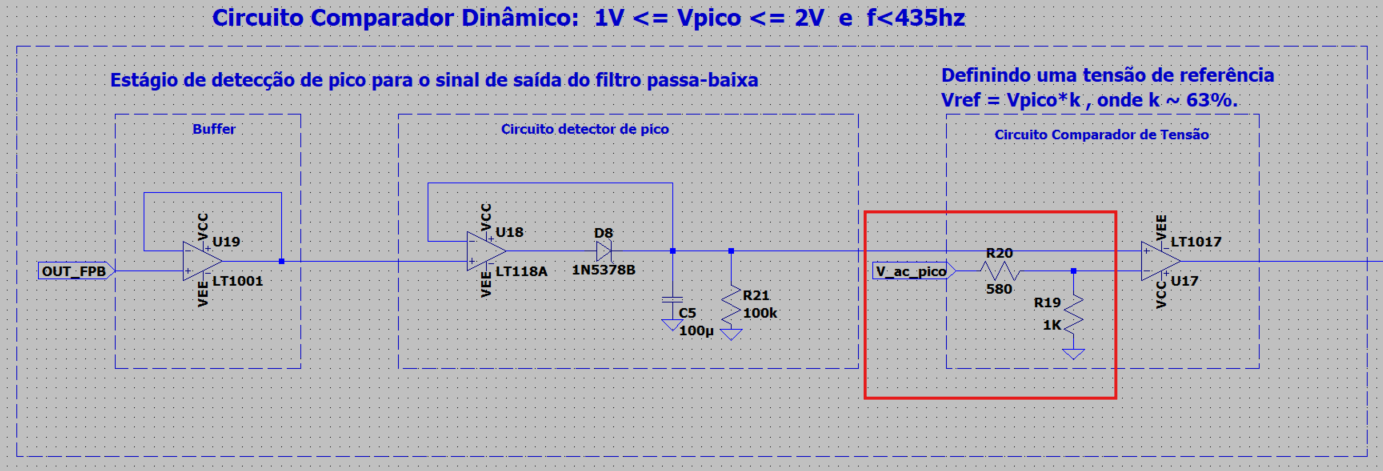
\includegraphics[scale=0.4]{imagens/circuito/comparador_dinamico_435hz.png}
        \caption{Circuito comparador dinâmico para f < 435hz}
    \end{figure}

    \item \textbf{Para o estágio de $f > 445hz$}:
    Escolhemos $R_2 = 1k \Omega$ e sabemos que $k \approx 50\%$, logo:
    \begin{equation*}
        k = 0.5 = \frac{1k}{R_1 + 1k}
    \end{equation*}
    \begin{equation*}
    R_1 \approx 1k\Omega
    \end{equation*}
    
    \begin{figure}[H]
        \centering
        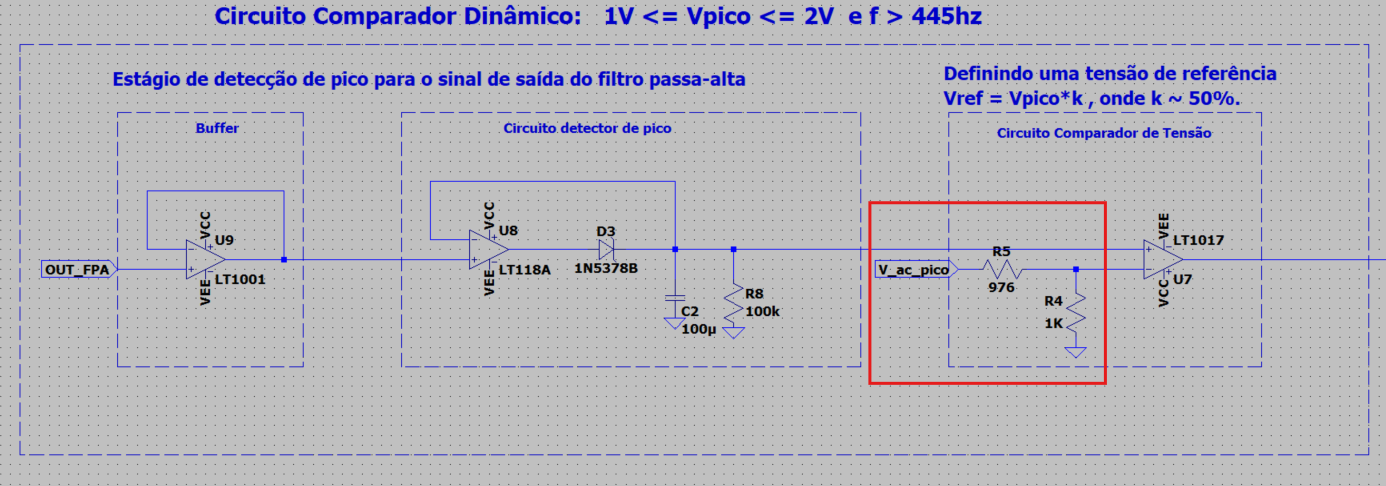
\includegraphics[scale=0.4]{imagens/circuito/comparador_dinamico_445hz.png}
        \caption{Circuito comparador dinâmico para f > 445hz}
    \end{figure}

    \item \textbf{Para o estágio de $ 435 \leq f \leq 445hz$}:
    Escolhemos $R_2 = 1k \Omega$ e sabemos que $k \approx 31.1\%$, logo:
    \begin{equation*}
        k = 0.5 = \frac{1k}{R_1 + 1k}
    \end{equation*}
    \begin{equation*}
    R_1 \approx 2.2k\Omega
    \end{equation*}
    
    \begin{figure}[H]
        \centering
        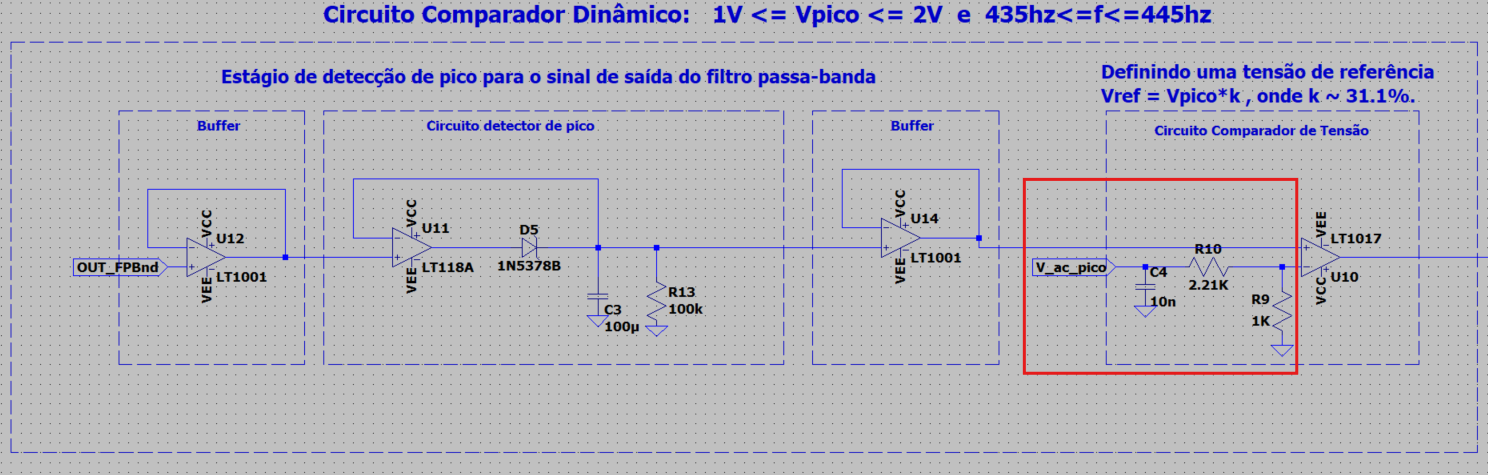
\includegraphics[scale=0.4]{imagens/circuito/comparador_dinamico_435-445hz.png}
        \caption{Circuito comparador dinâmico para $435 \leq f \leq 445$ }
    \end{figure}


\end{enumerate}




\subsubsection*{Exemplo de Operação:}
\begin{itemize}
    \item Para $V_{\mathrm{in}} = 1\, \mathrm{V}$:
    \begin{itemize}
        \item O detector de pico gera $V_{\mathrm{pico}} = 1\, \mathrm{V}$.
        \item O divisor resistivo ajusta $V_{\mathrm{ref}} \approx 0.63\, \mathrm{V}$.
        \item O comparador verifica se $V_{\mathrm{filtro}} < 0.63\, \mathrm{V}$ para acionar o LED.
    \end{itemize}
    \item Para $V_{\mathrm{in}} = 2\, \mathrm{V}$:
    \begin{itemize}
        \item O detector de pico gera $V_{\mathrm{pico}} = 2\, \mathrm{V}$.
        \item O divisor resistivo ajusta $V_{\mathrm{ref}} \approx 1.27\, \mathrm{V}$.
        \item O comparador verifica se $V_{\mathrm{filtro}} < 1.27\, \mathrm{V}$ para acionar o LED.
    \end{itemize}
\end{itemize}

Com esta abordagem, o circuito é capaz de operar dinamicamente para qualquer valor de entrada dentro do intervalo especificado, simplificando o projeto e garantindo a confiabilidade para diferentes amplitudes e frequências.



\subsubsection{Análise e Tratamento do Sinais Filtrados}

\begin{figure}[H]
\centering
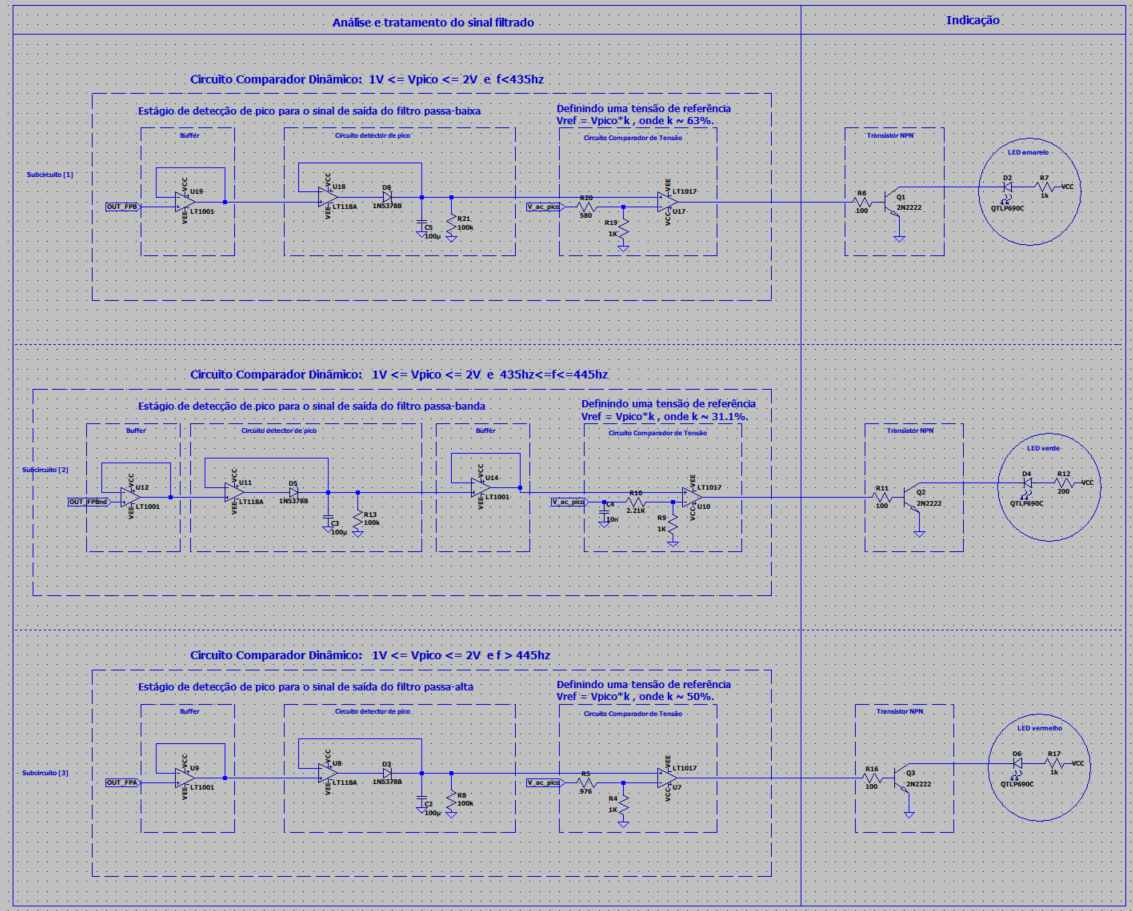
\includegraphics[scale=0.55]{imagens/circuito/tratamento_de_sinais_filtrados.png}
\caption{Circuitos de análise e tratamento dos sinais filtrados, com indicação visual.}
\end{figure}

Nesta parte, apresentamos os circuitos responsáveis pela análise e tratamento dos sinais filtrados, correspondendo às três faixas de frequência distintas (\(< 435 \, \mathrm{Hz}\), \(435 \, \mathrm{Hz} \leq f \leq 445 \, \mathrm{Hz}\), e \(f > 445 \, \mathrm{Hz}\)). Cada circuito é composto pelos seguintes estágios principais:


\begin{itemize}
    \item \textbf{Detecção de Pico:} Em cada faixa, o sinal filtrado passa por um circuito de detecção de pico, que utiliza amplificadores operacionais, diodos, resistores e capacitores. Esse estágio captura o valor de pico do sinal, essencial para a comparação subsequente.
    
    \item \textbf{Definição de Referência:} A partir do valor de pico detectado (\(V_{\mathrm{ac\_pico}}\)), uma tensão de referência (\(V_{\mathrm{ref}}\)) é gerada. Essa referência é determinada como uma fração específica (\(k\)) do valor de pico:
    \begin{itemize}
        \item \(k \approx 63\%\) para o filtro passa-baixa (\(< 435 \, \mathrm{Hz}\)).
        \item \(k \approx 31.1\%\) para o filtro passa-banda (\(435 \, \mathrm{Hz} \leq f \leq 445 \, \mathrm{Hz}\)).
        \item \(k \approx 50\%\) para o filtro passa-alta (\(f > 445 \, \mathrm{Hz}\)).
    \end{itemize}

    \item \textbf{Comparação de Tensão:} Comparadores de tensão verificam se \(V_{\mathrm{ac\_pico}}\) excede \(V_{\mathrm{ref}}\), acionando o estágio de indicação correspondente.

    \item \textbf{Indicação (LEDs):} 
    \begin{itemize}
        \item LED amarelo para frequências \(< 435 \, \mathrm{Hz}\).
        \item LED verde para frequências \(435 \, \mathrm{Hz} \leq f \leq 445 \, \mathrm{Hz}\).
        \item LED vermelho para frequências \(f > 445 \, \mathrm{Hz}\).
    \end{itemize}
\end{itemize}

Esse arranjo permite identificar visualmente a faixa de frequência do sinal de entrada após o tratamento, demonstrando a eficiência do sistema de filtragem e análise.



\subsection{Simulação Transiente}

A simulação transiente foi realizada com o objetivo de validar o comportamento dinâmico do circuito frente a sinais de entrada variando em frequência e amplitude. Esse tipo de análise permite observar, em detalhe, a evolução temporal das grandezas elétricas, como tensão e corrente, em cada estágio do circuito.\\

No contexto deste projeto, a simulação transiente é particularmente relevante para avaliar:

\begin{itemize}
    \item O desempenho do circuito em diferentes faixas de frequência, especialmente nos limites definidos para a afinação.
    \item A resposta dos LEDs indicadores, que sinalizam frequências fora da faixa esperada.
\end{itemize}

Os resultados das simulações transientes mostram a interação entre os elementos do circuito, como os detectores de pico, comparadores de tensão e componentes de indicação visual (LEDs). Essas simulações são fundamentais para verificar o funcionamento correto e garantir a confiabilidade do circuito em condições reais de operação.


\subsubsection{Desafinado Para Baixo: $f < 435$}

A análise para frequências abaixo de 435 Hz apresentou um comportamento bastante preciso, evidenciando a eficácia do circuito projetado para o LED amarelo. Observou-se que a faixa de resposta está bem ajustada, com o LED apagando progressivamente conforme a frequência diminui. 

\begin{itemize}
    \item \textbf{Tensão senoidal de 1V}:

    \begin{itemize}
        \item \textbf{f = 430Hz}:
        Exatamente em 430Hz, a simulação mostra o LED amarelo acendendo de forma consistente, validando o funcionamento correto do circuito comparador e filtro passa-baixa. Na imagem, podemos perceber a continuidade em torno de 10mA e 1.8V.

        \begin{figure}[H]
            \centering
            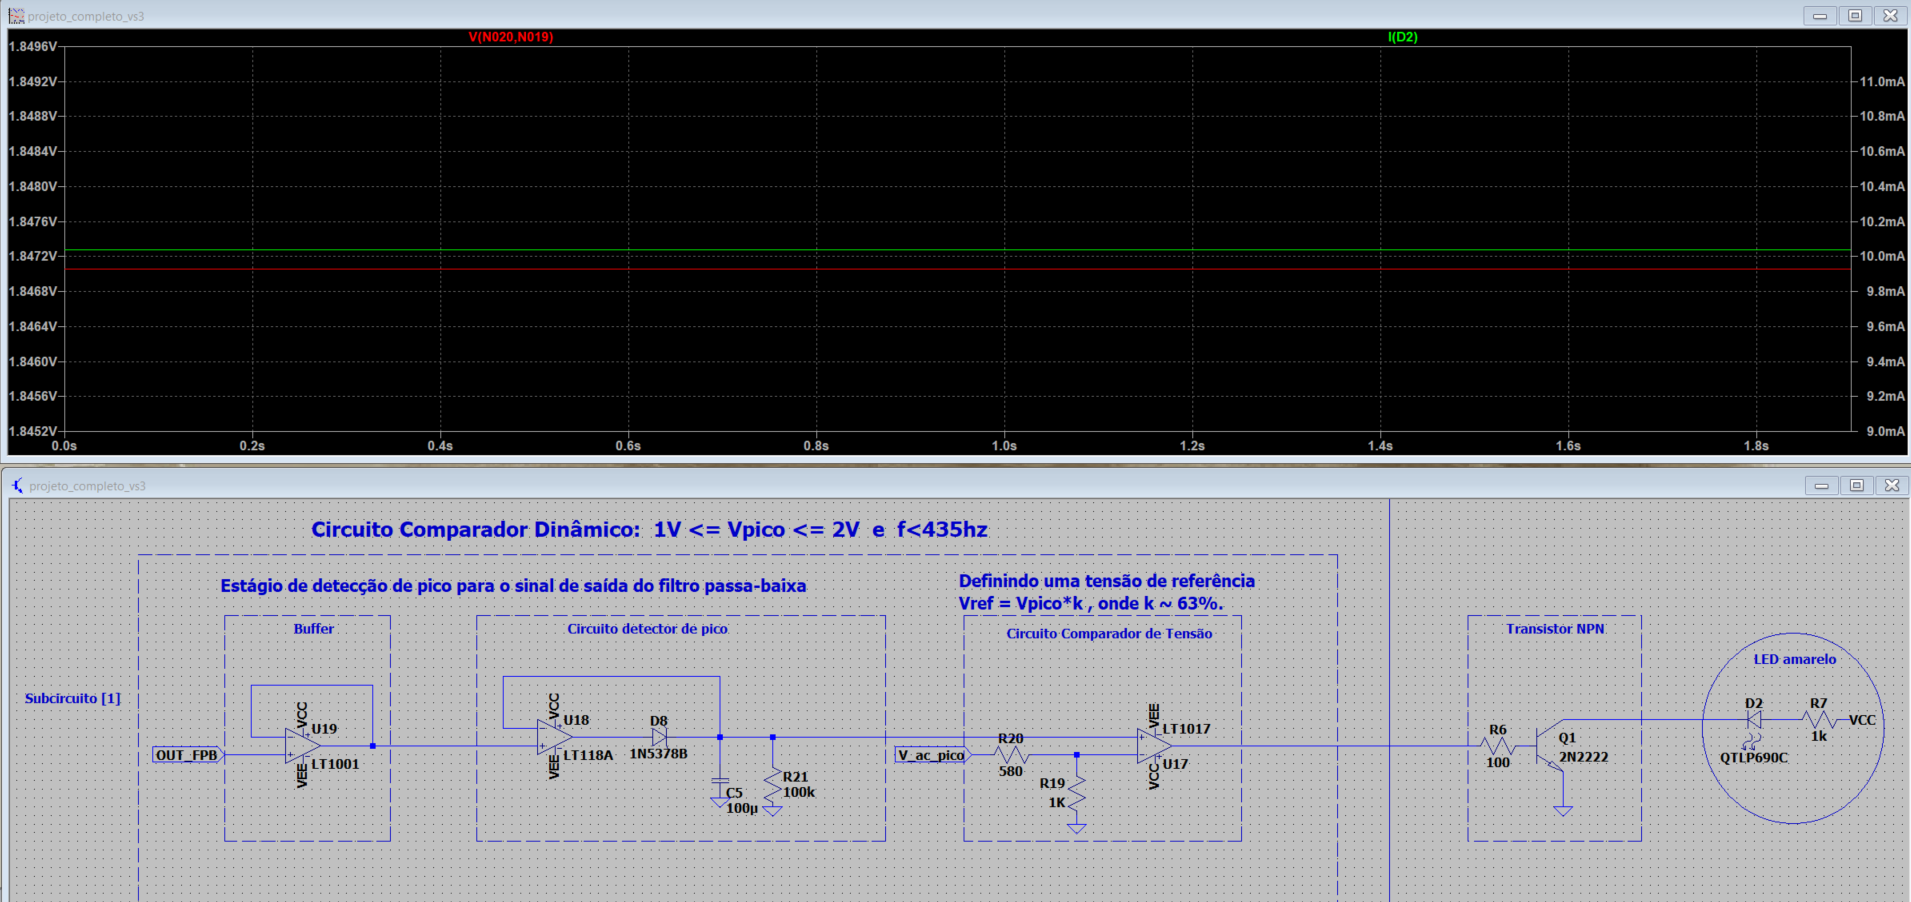
\includegraphics[scale=0.3]{imagens/graficos/simu_1v_430hz_passa-baixa.png}
            \caption{Simulação do LED amarelo: 1V a 430Hz}
        \end{figure}

        \item \textbf{f = 435Hz}:
        Em 435hz, o LED amarelo está na iminência de apagar completamente, pois apresenta oscilações na corrente que passa pelo mesmo, bem como na tensão em seus terminais, como observa-se no gráfico.
        \begin{figure}[H]
            \centering
            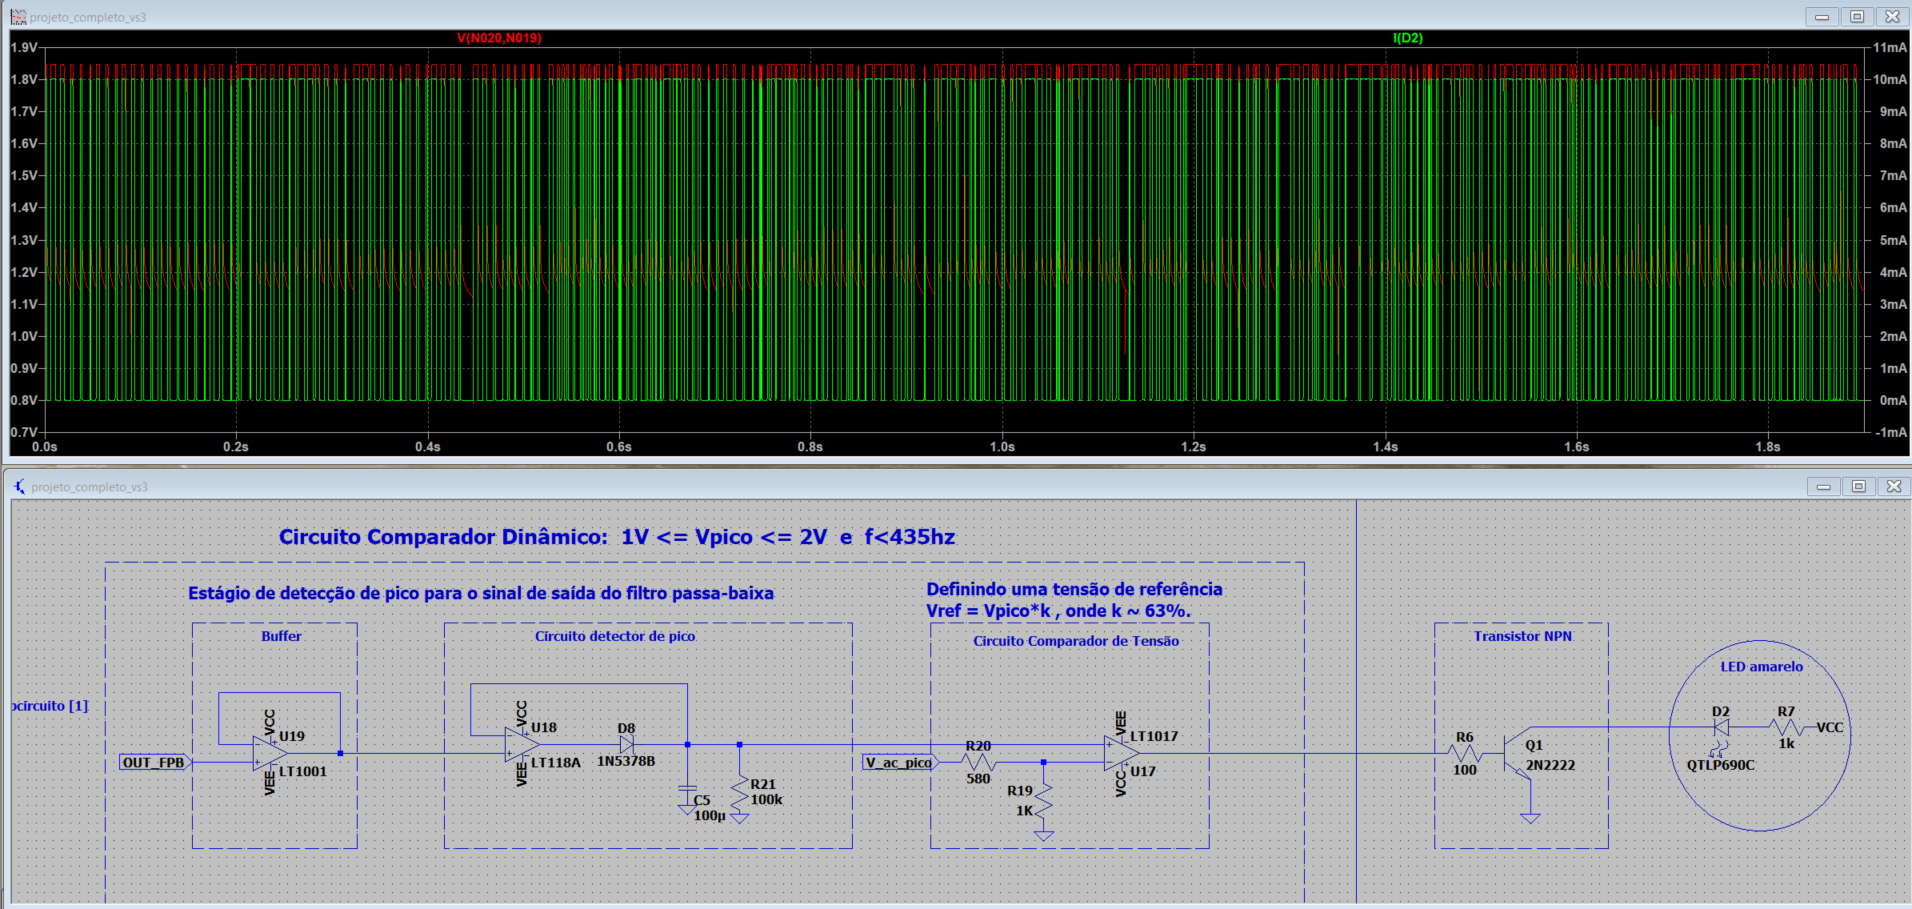
\includegraphics[scale=0.3]{imagens/graficos/simu_1v_435hz_passa-baixa.png}
            \caption{Simulação do LED amarelo: 1V a 435Hz}
        \end{figure}

        \item \textbf{f = 440Hz}:
        Para frequências acima de 440Hz, o LED amarelo já está apagado, confirmando que o filtro passa-baixa atua eficientemente para atenuar sinais fora da faixa desejada.
        \begin{figure}[H]
            \centering
            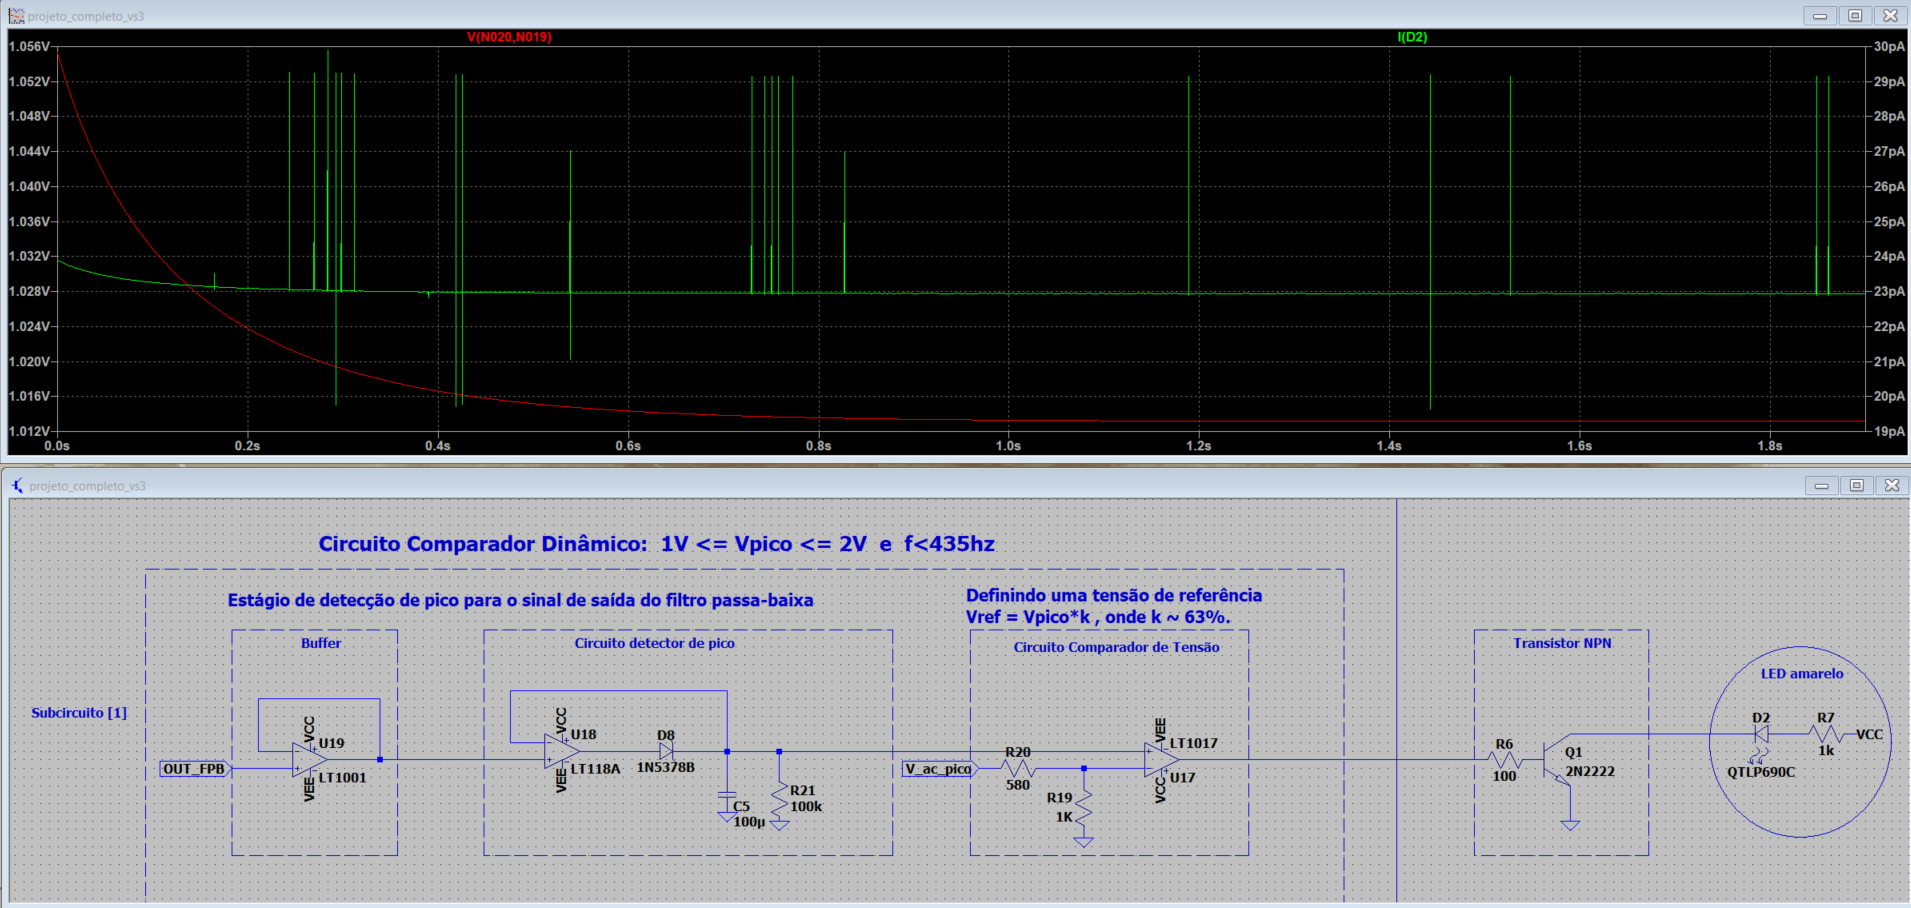
\includegraphics[scale=0.3]{imagens/graficos/simu_1v_440hz_passa-baixa.png}
            \caption{Simulação do LED amarelo: 1V a 440Hz}
        \end{figure}
        
    \end{itemize}
\end{itemize}      

\begin{itemize}
    \item \textbf{Tensão senoidal de 2V}:
    \begin{itemize}

        \item \textbf{f = 430Hz}:
        A 430Hz, o LED amarelo acende de forma consistente, indicando que o valor de pico foi corretamente detectado e comparado com sucesso pelo circuito.

        \begin{figure}[H]
            \centering
            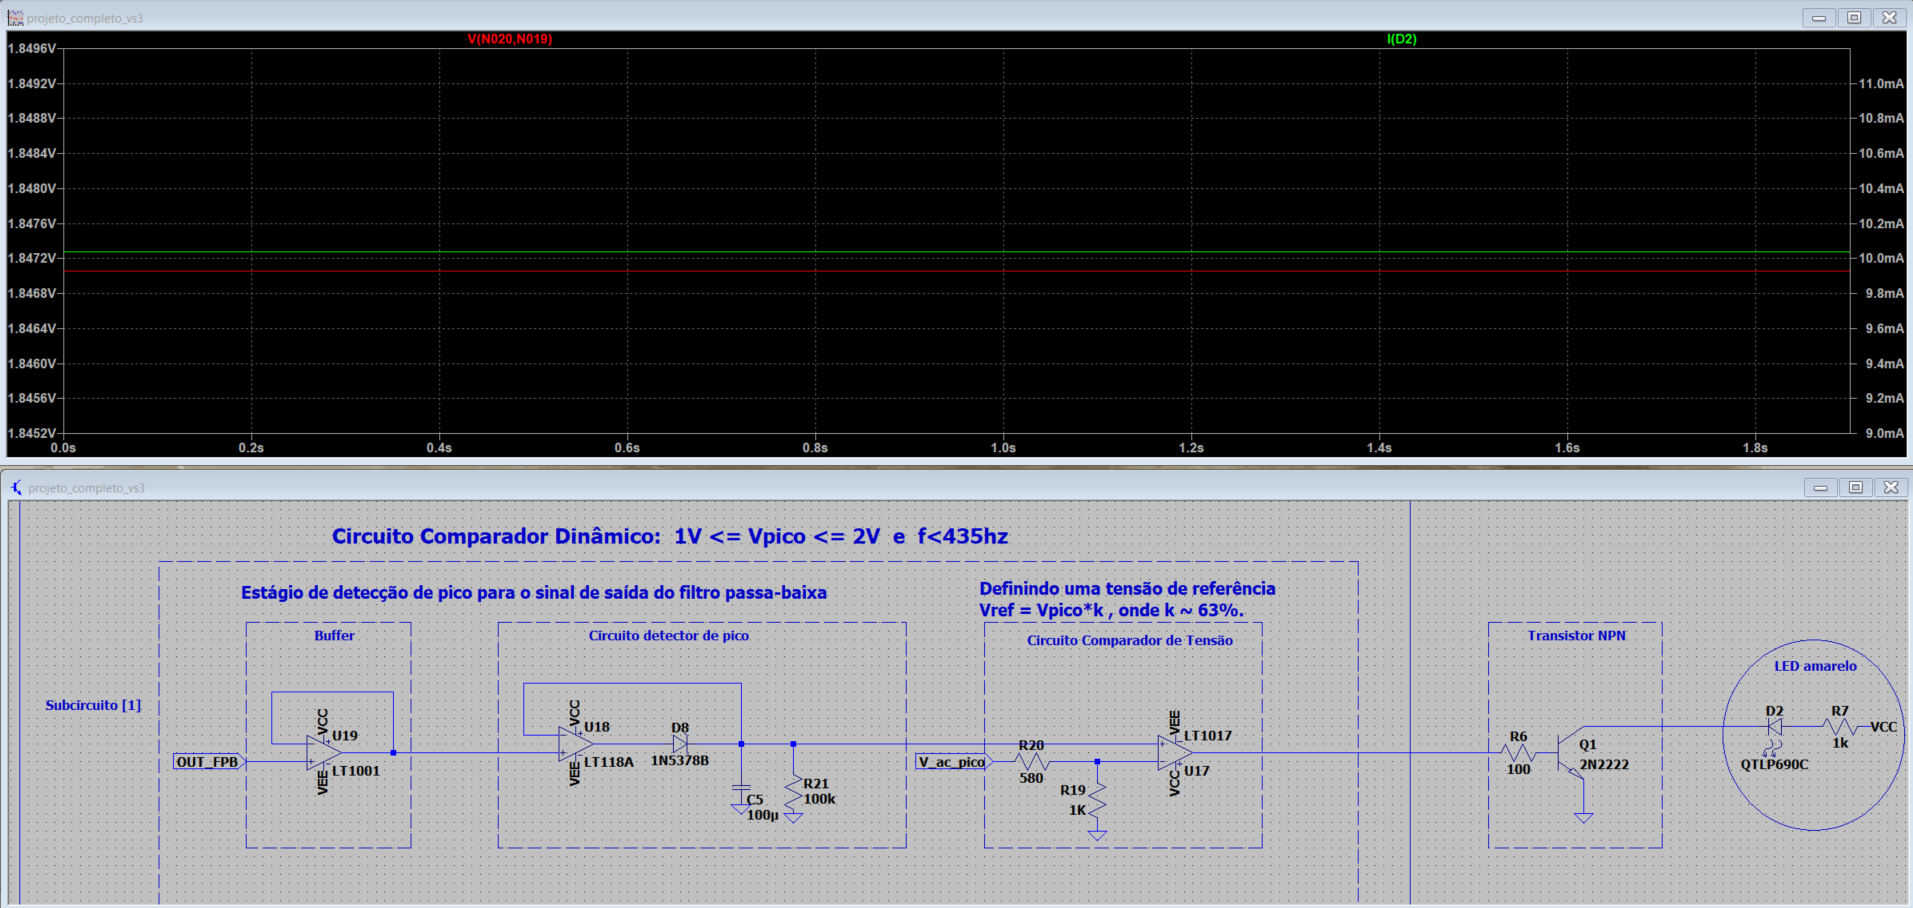
\includegraphics[scale=0.3]{imagens/graficos/simu_2v_430hz_passa-baixa.png}
            \caption{Simulação do LED amarelo: 2V a 430Hz}
        \end{figure}

        \item \textbf{f = 435Hz}:
        Em 435Hz com 2V, o LED amarelo também começa a responder levemente, mostrando que o circuito mantém sua funcionalidade mesmo em níveis de tensão mais elevados.
        
        \begin{figure}[H]
            \centering
            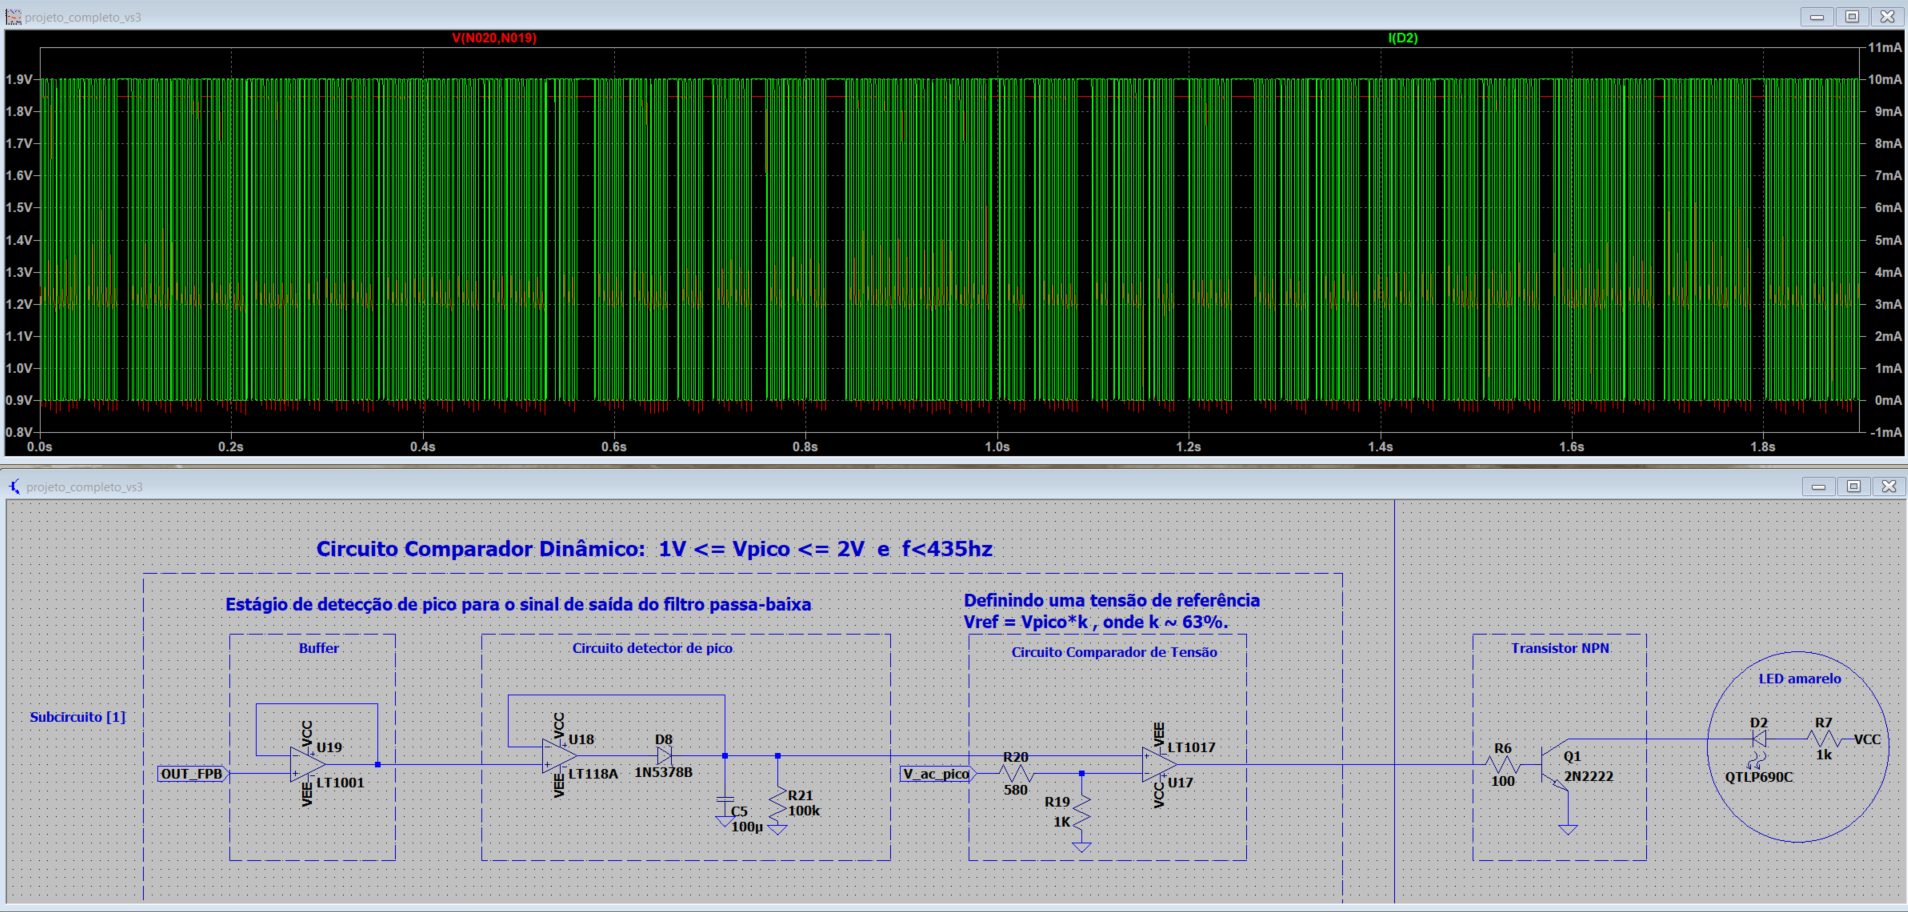
\includegraphics[scale=0.3]{imagens/graficos/simu_2v_435hz_passa-baixa.png}
            \caption{Simulação do LED amarelo: 2V a 435Hz}
        \end{figure}

        
        \item \textbf{f = 440Hz}:
        Em 440Hz, o LED amarelo já não acende, novamente validando o corte eficaz do filtro passa-baixa para sinais abaixo da frequência de corte projetada.
        
        \begin{figure}[H]
            \centering
            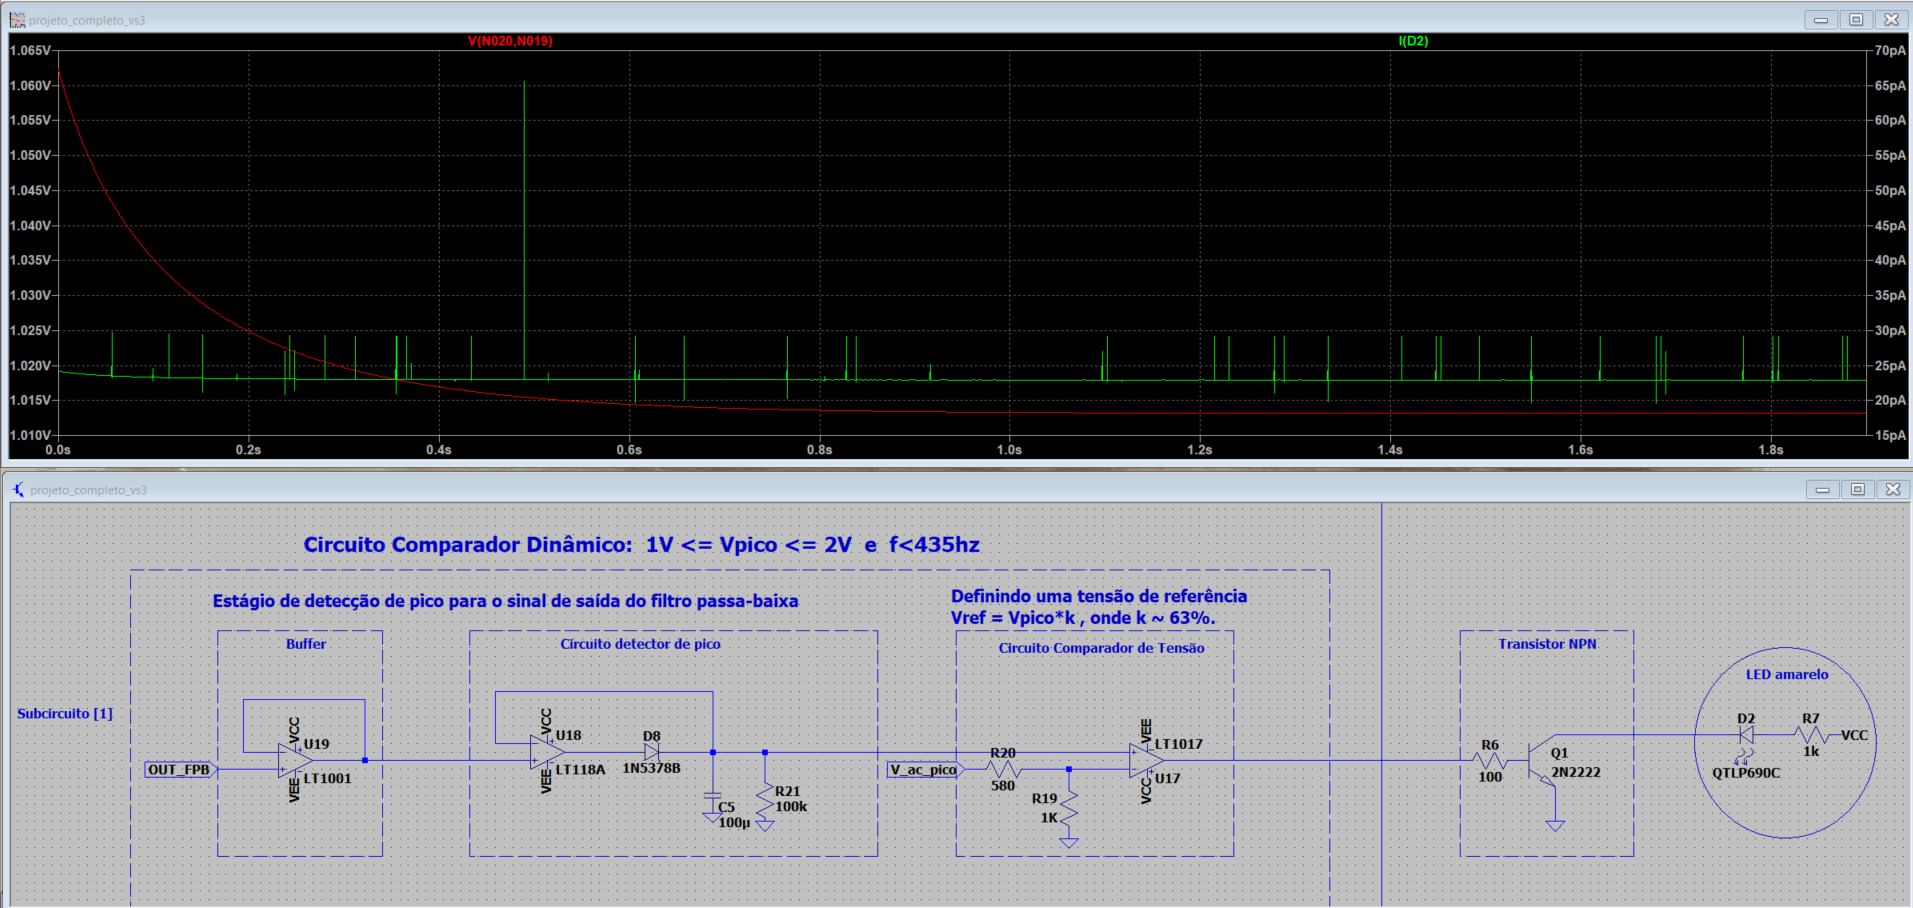
\includegraphics[scale=0.3]{imagens/graficos/simu_2v_440hz_passa-baixa.png}
            \caption{Simulação do LED amarelo: 2V a 440Hz}
        \end{figure}
\end{itemize}
\end{itemize}

O comportamento observado é consistente com os cálculos e parâmetros projetados para o filtro passa-baixa e comparador de tensão. O LED amarelo apresenta alta precisão e eficiência na faixa definida, comprovando que o circuito é funcional e bem ajustado para identificar frequências abaixo de 435Hz. O filtro passa-baixa desempenha um papel crucial ao garantir que o sinal de saída esteja alinhado com os critérios do circuito comparador, permitindo uma resposta clara e confiável do LED.



\subsubsection{Desafinado Para Cima: $f > 445hz$}

A análise para frequências acima de 445hz também apresentou um comportamento bastante preciso, evidenciando a eficácia do circuito projetado para o LED vermelho.

\begin{itemize}
    \item \textbf{Tensão senoidal = 1V}:
    \begin{itemize}
        \item \textbf{f = 440hz}:        
        Nesta simulação, o LED vermelho permanece apagado como esperado, indicando que a frequência está abaixo do limite superior definido pelo circuito.
        \begin{figure}[H]
            \centering
            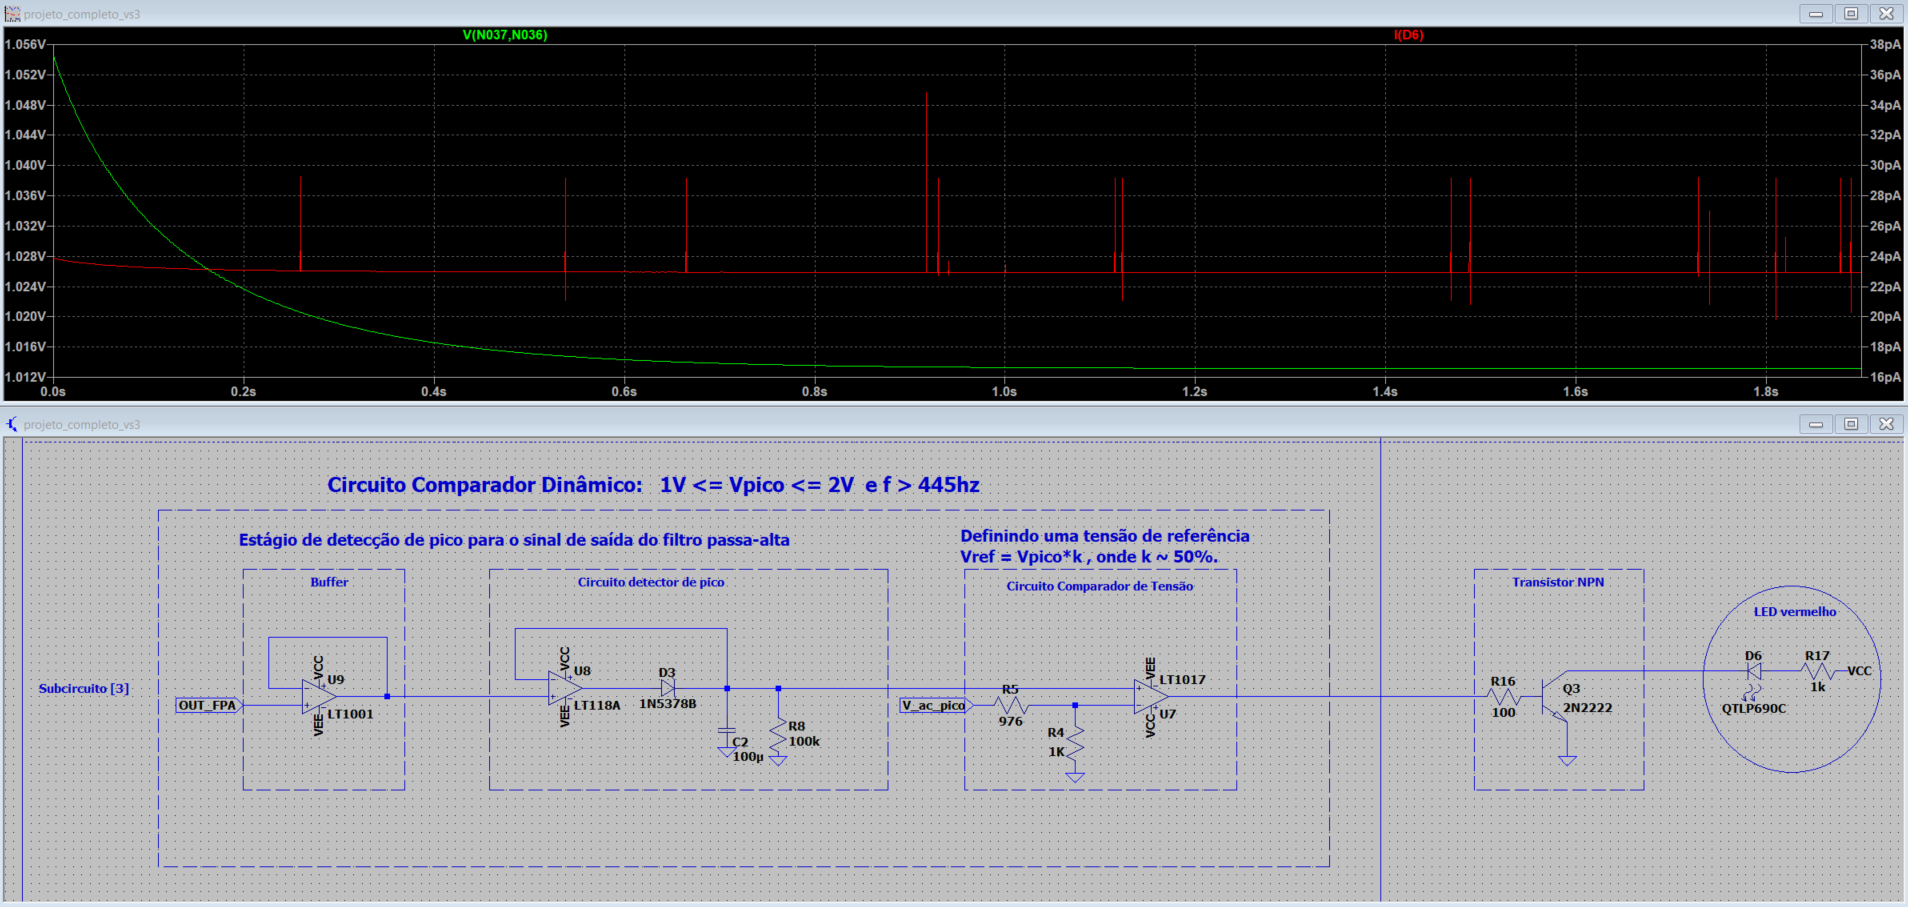
\includegraphics[scale=0.3]{imagens/graficos/simu_1v_440hz_passa-alta.png}
            \caption{Simulação do LED vermelho: 1V a 440hz}
        \end{figure}


        \item \textbf{f = 445hz}:
        Com a frequência atingindo exatamente 445Hz, o LED vermelho encontra-se na iminência de acender, mostrando que o circuito está atuando com alta sensibilidade na detecção de frequências superiores ao limiar.
        \begin{figure}[H]
            \centering
            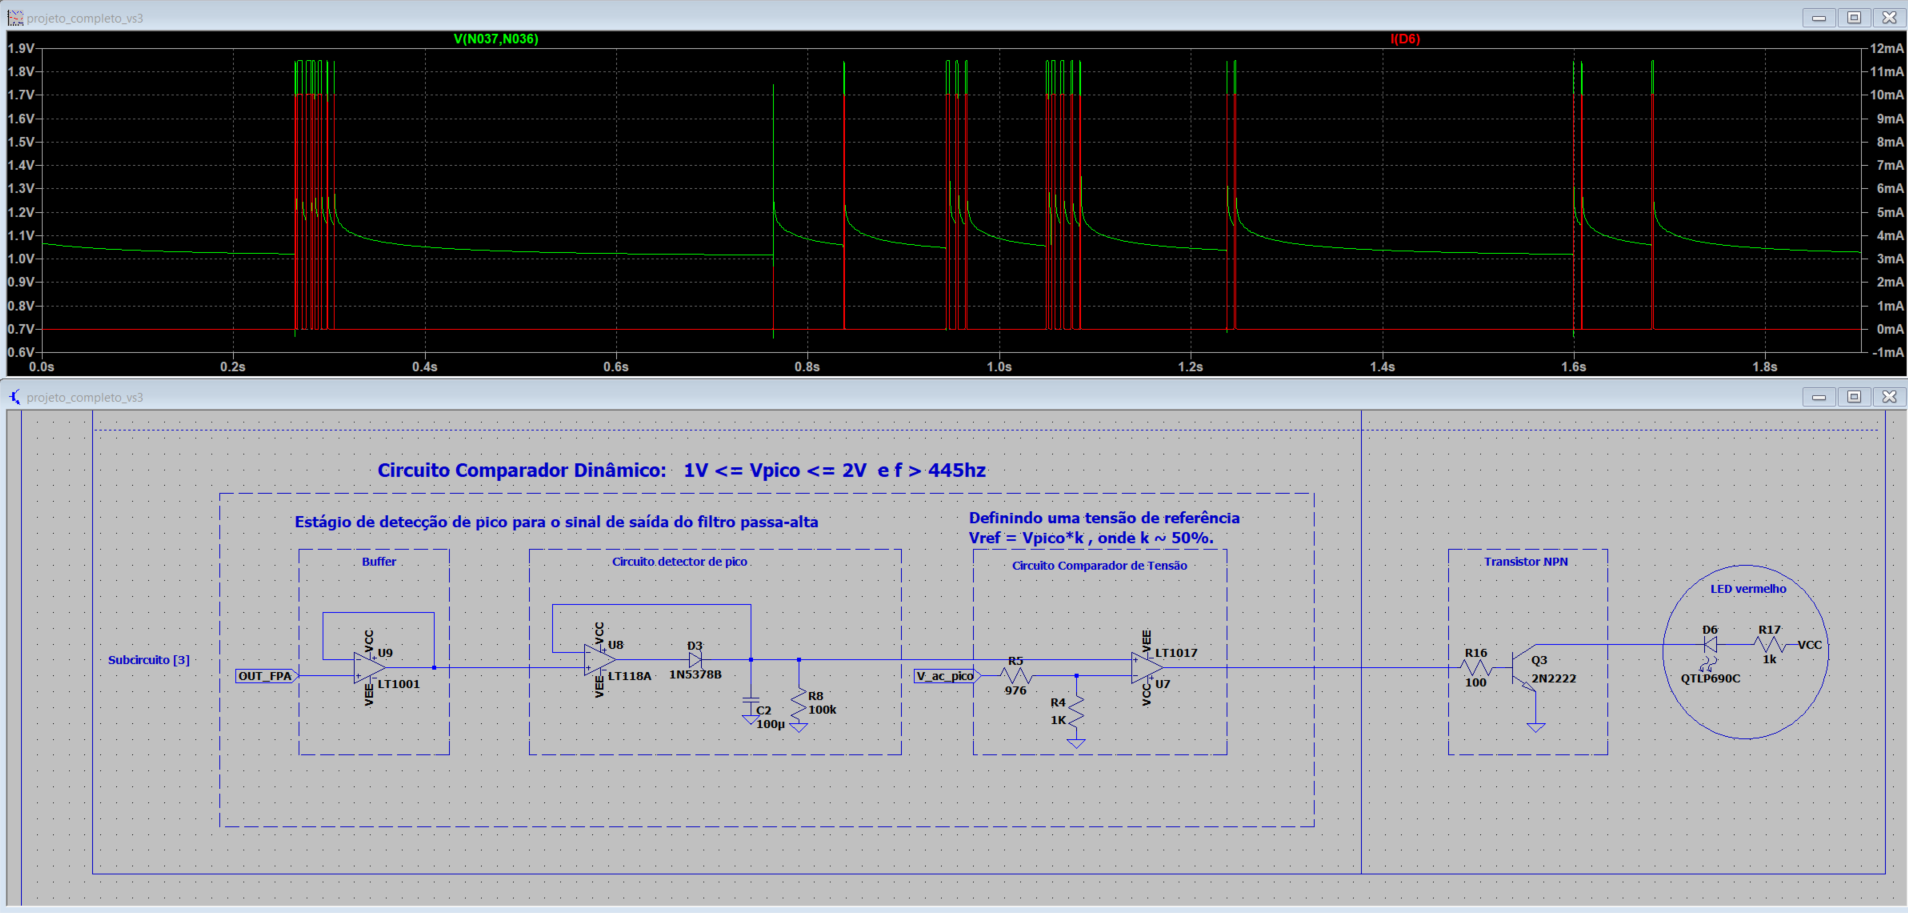
\includegraphics[scale=0.3]{imagens/graficos/simu_1v_445hz_passa-alta.png}
            \caption{Simulação do LED vermelho: 1V a 445hz}
        \end{figure}
        

        \item \textbf{f = 450hz}:
        A partir de 450Hz, o LED vermelho já se mantém aceso, embora não tão fortemente, confirmando o correto funcionamento do circuito na identificação de frequências fora da faixa esperada.
        \begin{figure}[H]
            \centering
            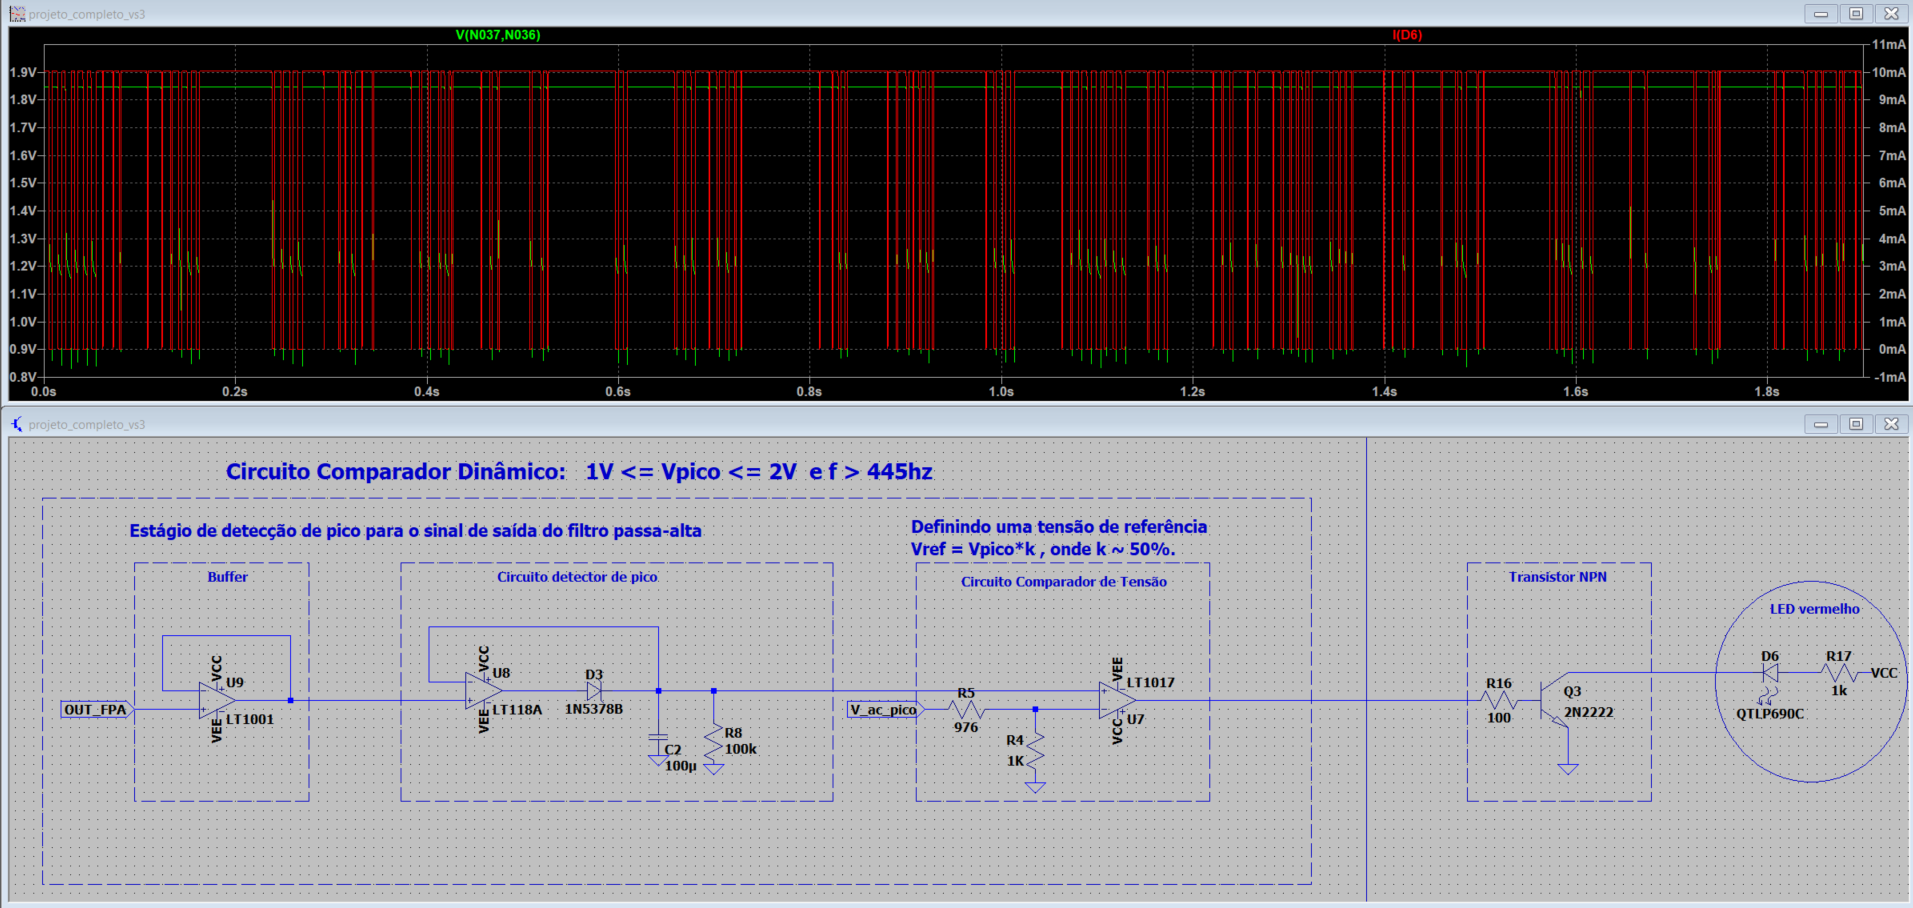
\includegraphics[scale=0.3]{imagens/graficos/simu_1v_450hz_passa-alta.png}
            \caption{Simulação do LED vermelho: 1V a 450hz}
        \end{figure}
        

        \item \textbf{f = 455hz}:
        Nesta frequência, o LED vermelho já mantém-se aceso consistentemente, reforçando a confiabilidade do circuito em detectar frequências acima do limite de 445Hz.
        \begin{figure}[H]
            \centering
            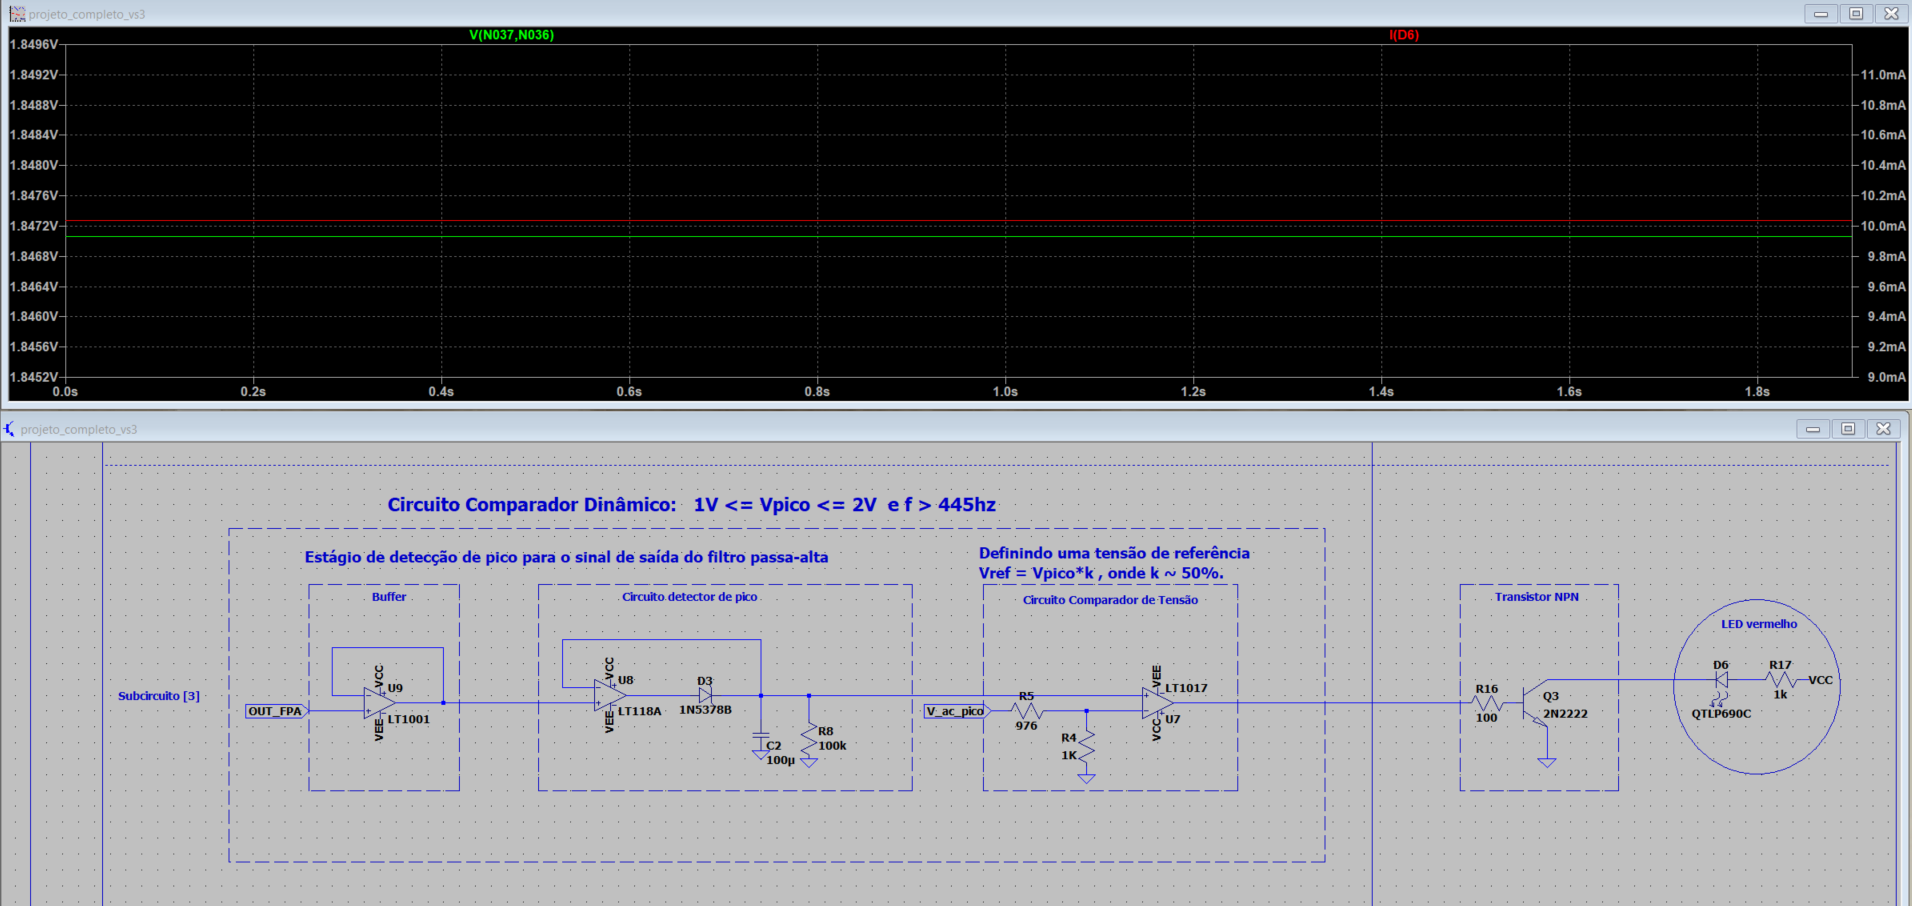
\includegraphics[scale=0.3]{imagens/graficos/simu_1v_455hz_passa-alta.png}
            \caption{Simulação do LED vermelho: 1V a 455hz}
        \end{figure}
        
    \end{itemize}
\end{itemize}

\begin{itemize}
    \item \textbf{Tensão senoidal = 2V}:
    \begin{itemize}
        \item \textbf{f = 440hz}:
        Assim como na tensão de 1V, o LED vermelho permanece apagado em 440Hz, confirmando o comportamento esperado para frequências dentro do limite.
        \begin{figure}[H]
            \centering
            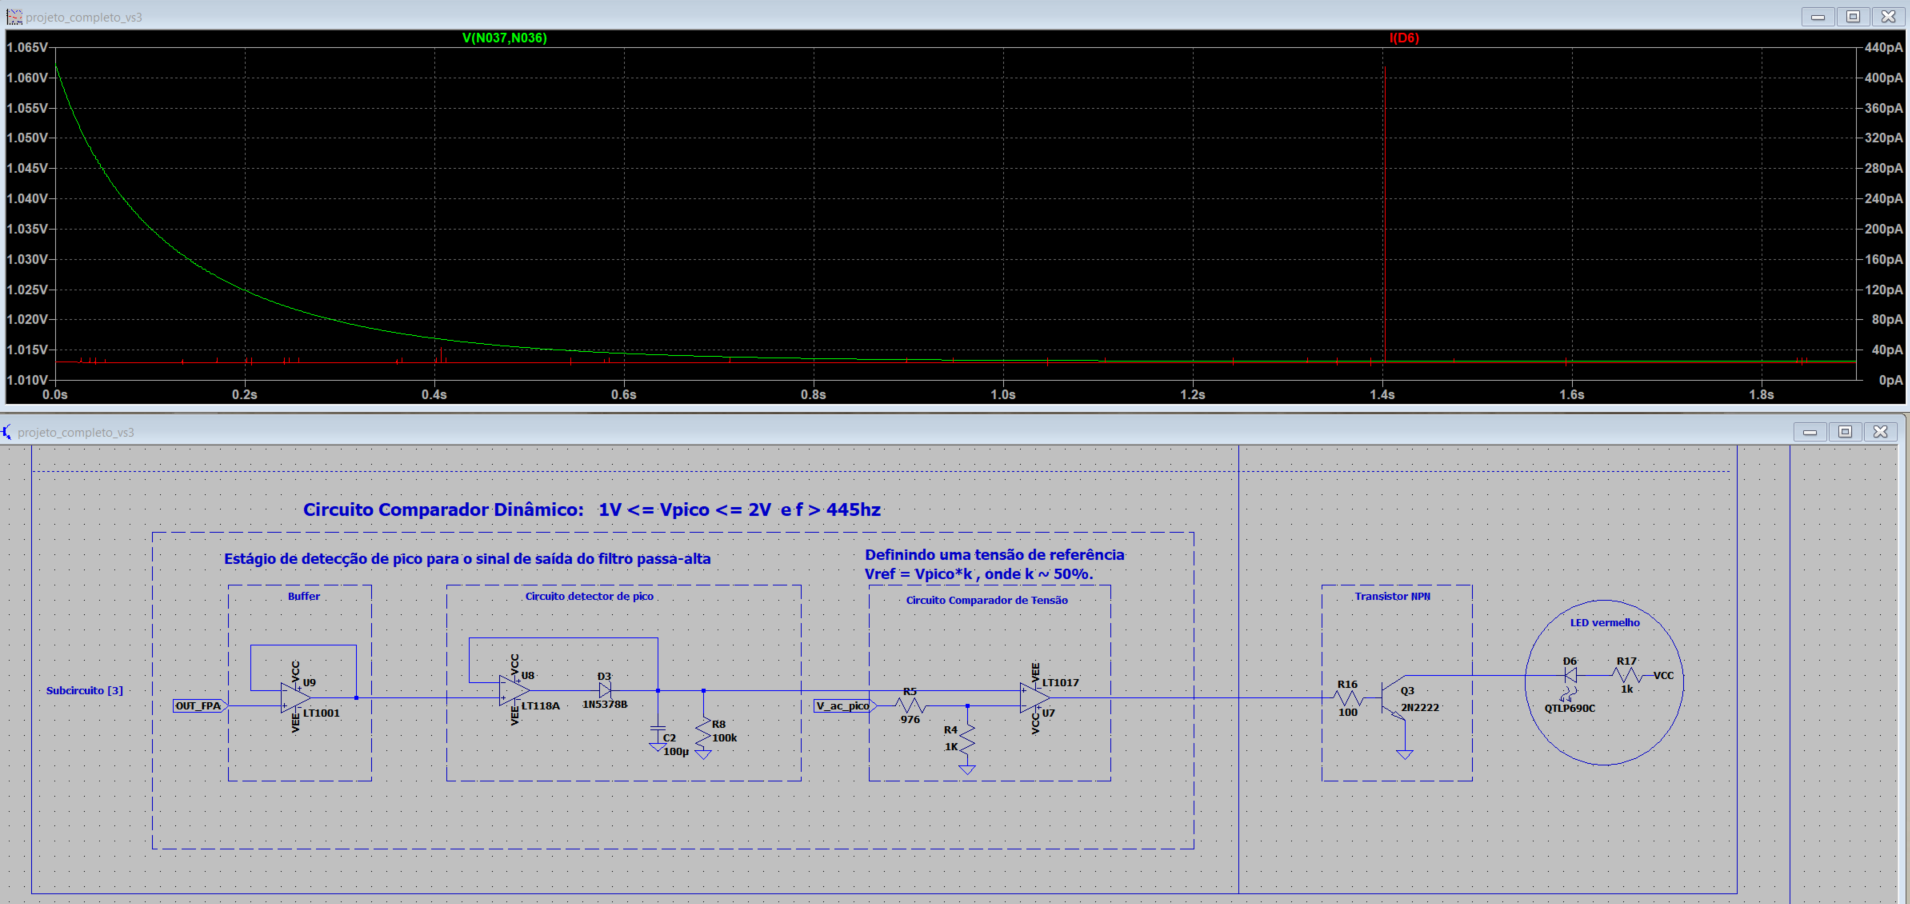
\includegraphics[scale=0.3]{imagens/graficos/simu_2v_440hz_passa-alta.png}
            \caption{Simulação do LED vermelho: 2V a 440hz}
        \end{figure}
        

        \item \textbf{f = 445hz}:
        Em 445Hz e 2V, o LED vermelho encontra-se ainda apagado, reforçando o desempenho consistente do circuito ao detectar frequências no limite.
        \begin{figure}[H]
            \centering
            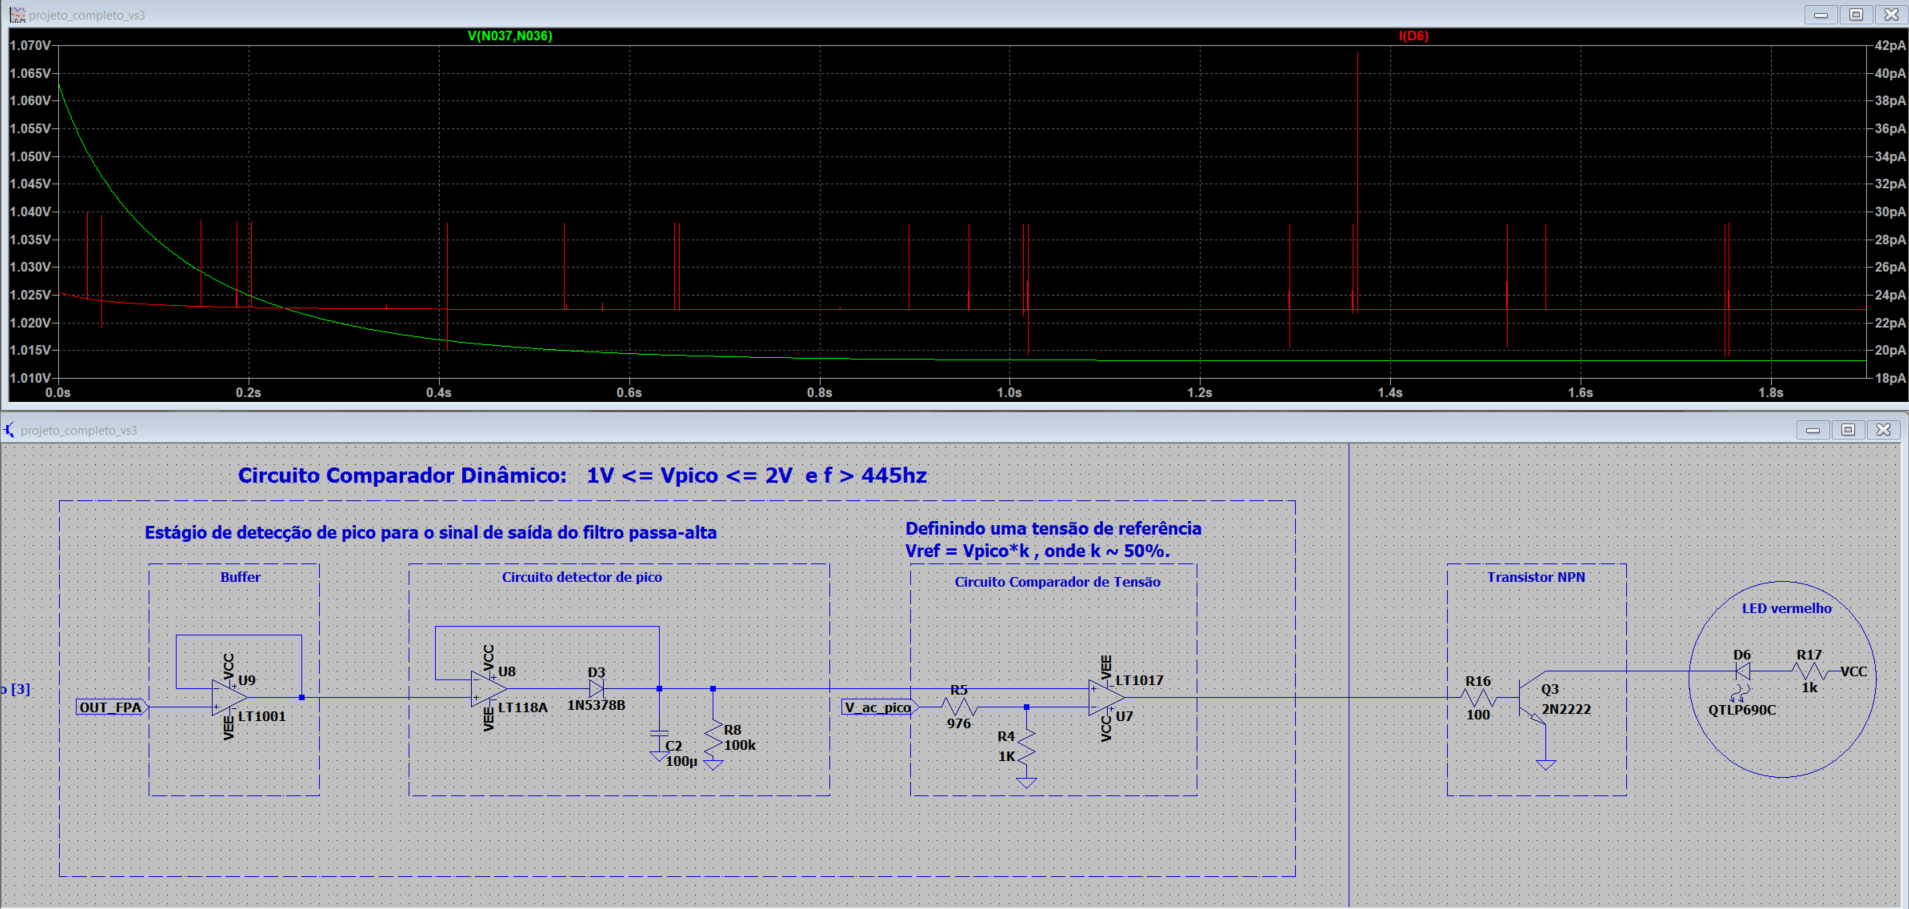
\includegraphics[scale=0.3]{imagens/graficos/simu_2v_445hz_passa-alta.png}
            \caption{Simulação do LED vermelho: 2V a 445hz}
        \end{figure}
        

        \item \textbf{f = 450hz}:
        Para 450Hz e tensão de 2V, o LED vermelho já mantém-se aceso de forma contínua, evidenciando o funcionamento preciso do circuito em frequências acima do limite.
        \begin{figure}[H]
            \centering
            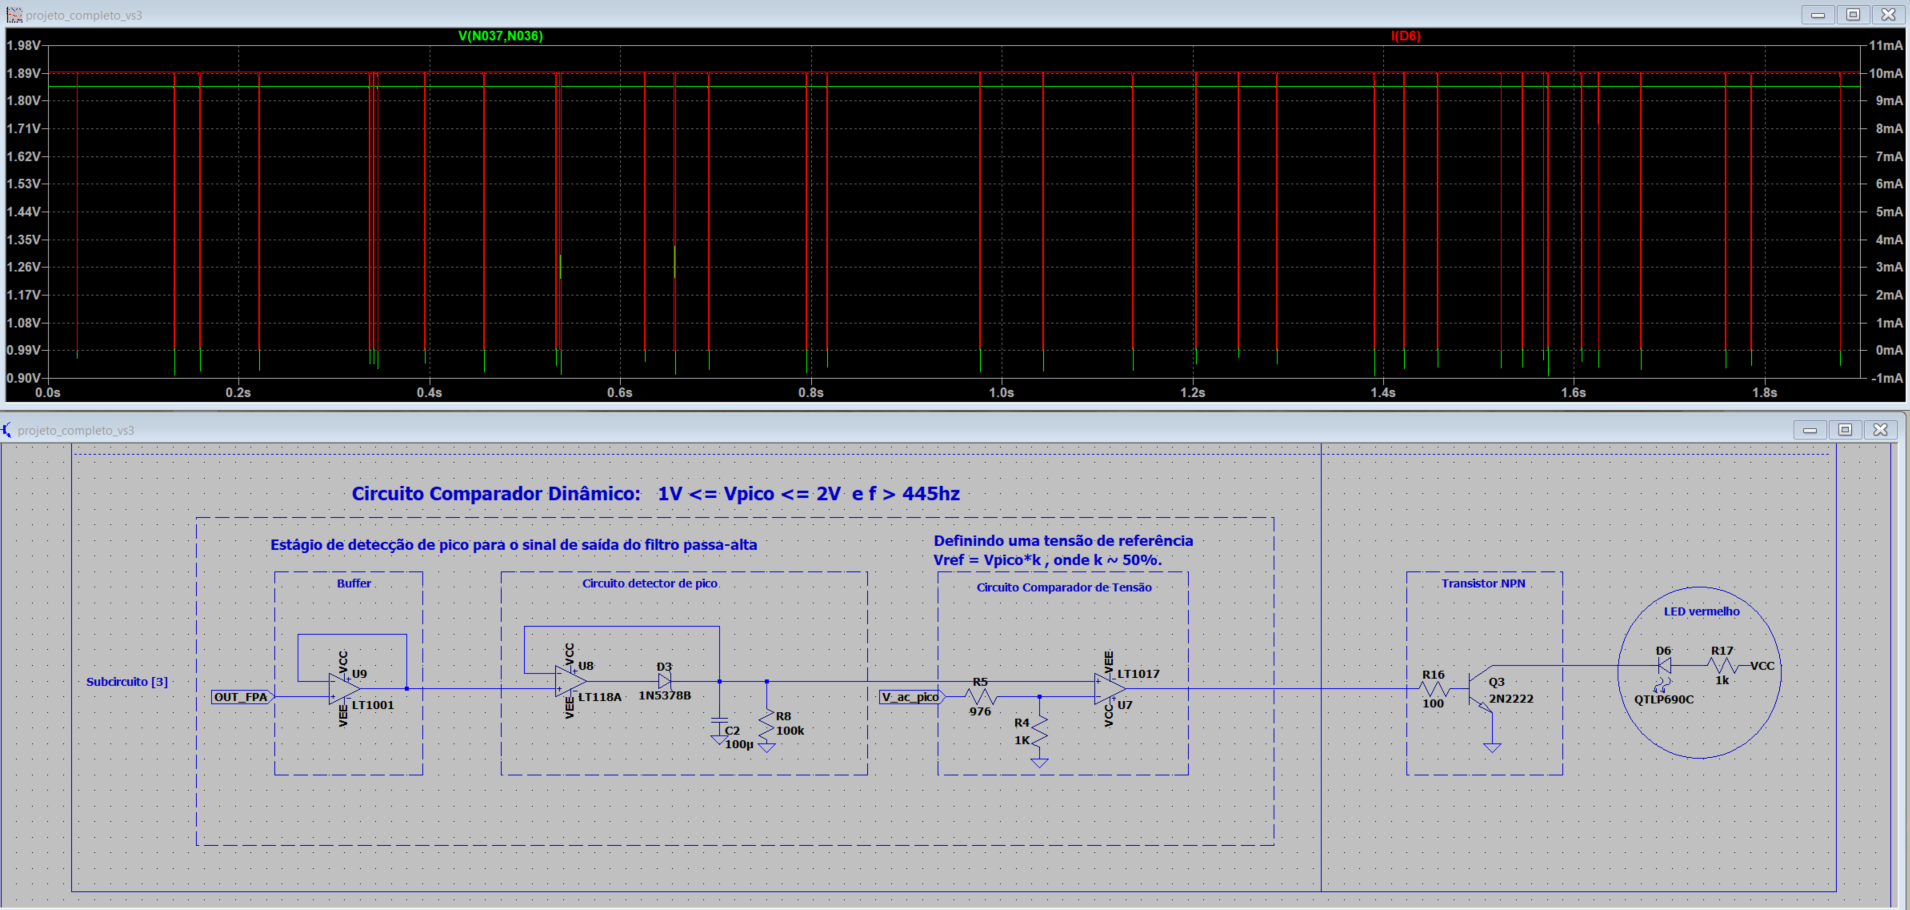
\includegraphics[scale=0.3]{imagens/graficos/simu_2v_450hz_passa-alta.png}
            \caption{Simulação do LED vermelho: 2V a 450hz}
        \end{figure}
        

        \item \textbf{f = 455hz}:
        Em 455Hz, o LED vermelho segue aceso, agora com mais intensidade e sem oscilações, confirmando a operação confiável do circuito para frequências significativamente superiores a 445Hz.
        \begin{figure}[H]
            \centering
            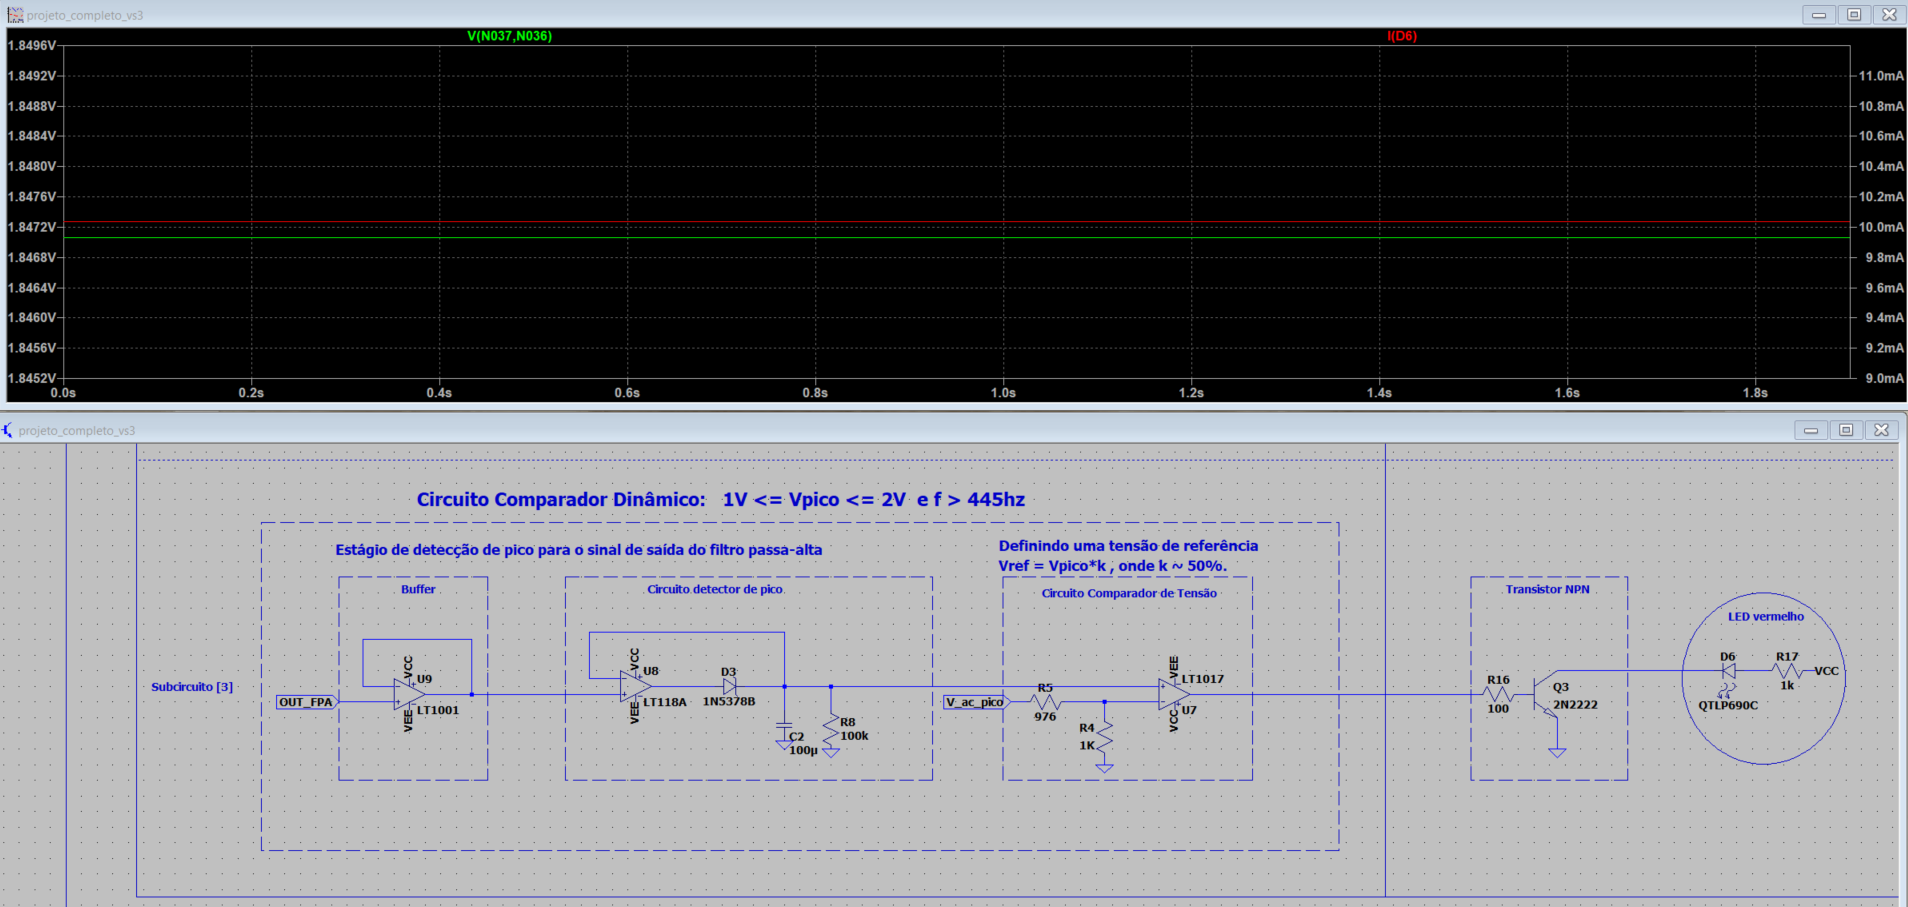
\includegraphics[scale=0.3]{imagens/graficos/simu_2v_455hz_passa-alta.png}
            \caption{Simulação do LED vermelho: 2V a 455hz}
        \end{figure}
        
    \end{itemize}

    A análise para o caso de $f>445Hz$ demonstra que o circuito está funcionando conforme o esperado, principalmente na detecção de frequências fora da faixa de afinação desejada.
\end{itemize}


\subsubsection{Afinado: $435hz \leq f \leq 445hz$}

Mesmo com os ajustes realizados, o LED verde apresentou um comportamento de piscar em frequências próximas a 440 Hz. Esse comportamento se deve às pequenas oscilações do sinal detectado no circuito de pico e possíveis tolerâncias nos componentes responsáveis pela referência de tensão.

Apesar disso, o sistema ainda é funcional no contexto geral. Quando o LED verde está piscando, indica que a frequência está próxima da faixa afinada. A confirmação de uma afinação precisa ocorre quando os LEDs vermelho e amarelo permanecem apagados, garantindo que a frequência esteja entre 435 Hz e 445 Hz.

\begin{itemize}
    \item \textbf{Tensão senoidal = 1V}:
    \begin{itemize}
        \item \textbf{f = 445hz}:
        \begin{figure}[H]
        \centering
            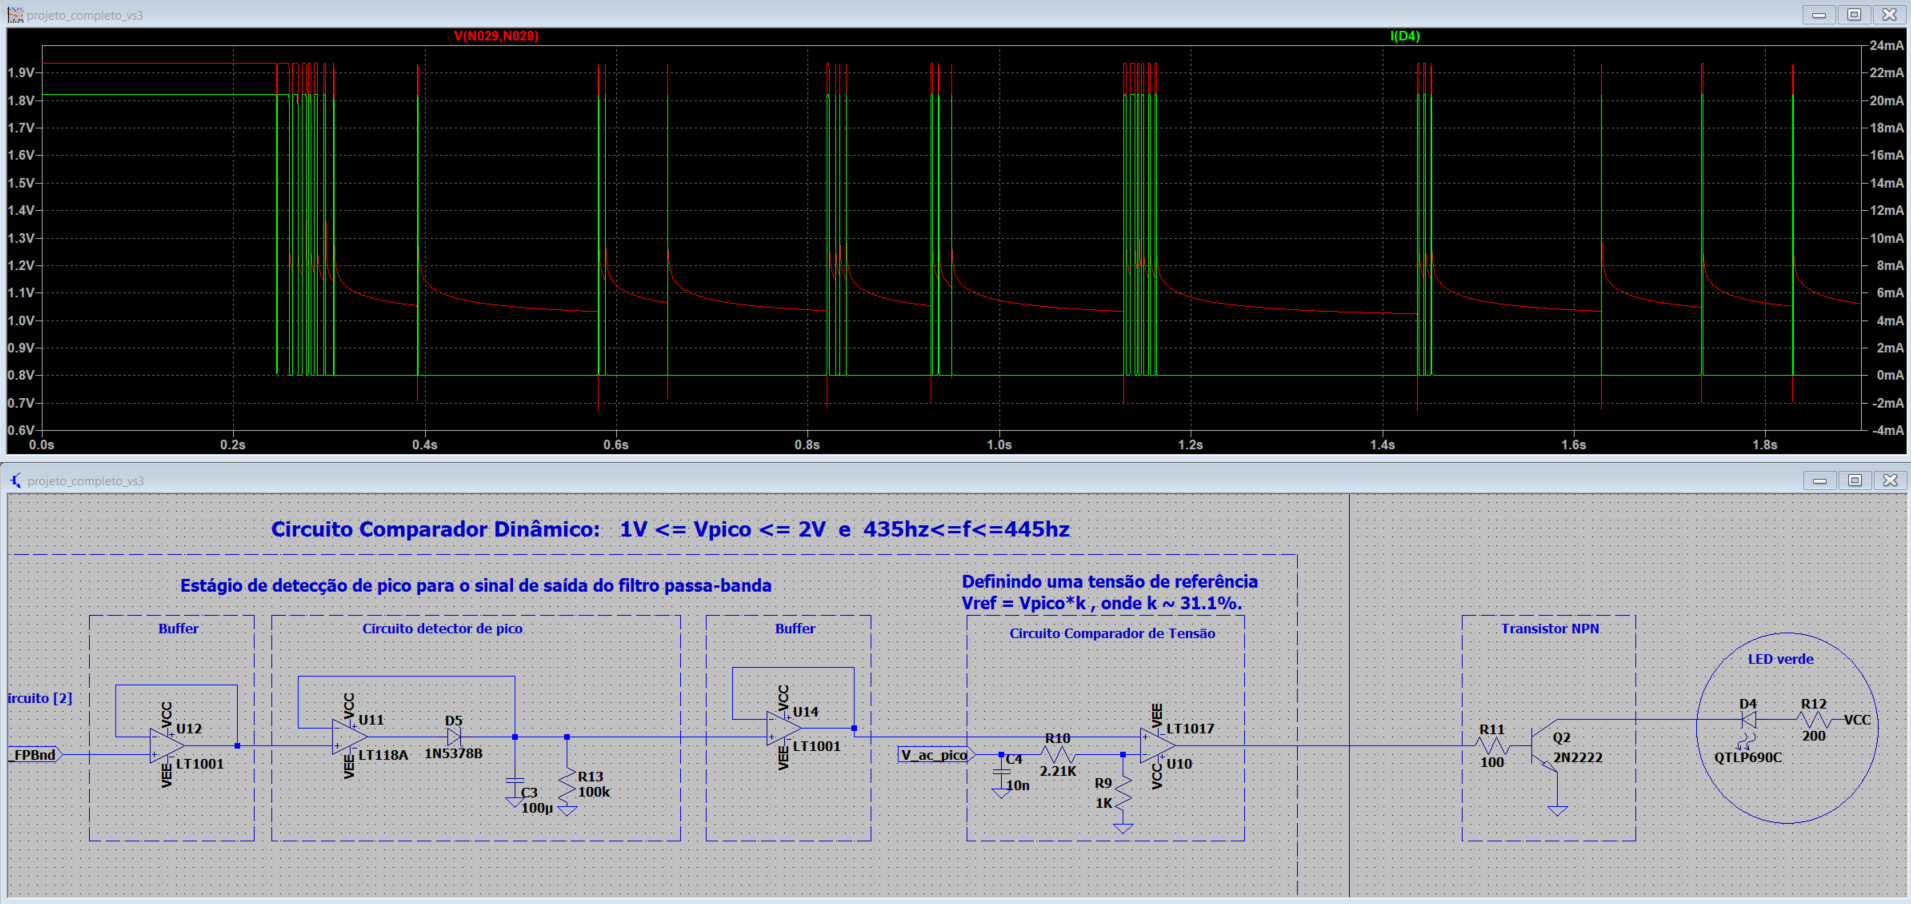
\includegraphics[scale=0.3]{imagens/graficos/simu_1v_445hz_passa-banda.png}
            \caption{Simulação do LED verde: 1V a 445hz}
        \end{figure}

        \item \textbf{f = 440hz}:
        \begin{figure}[H]
        \centering
            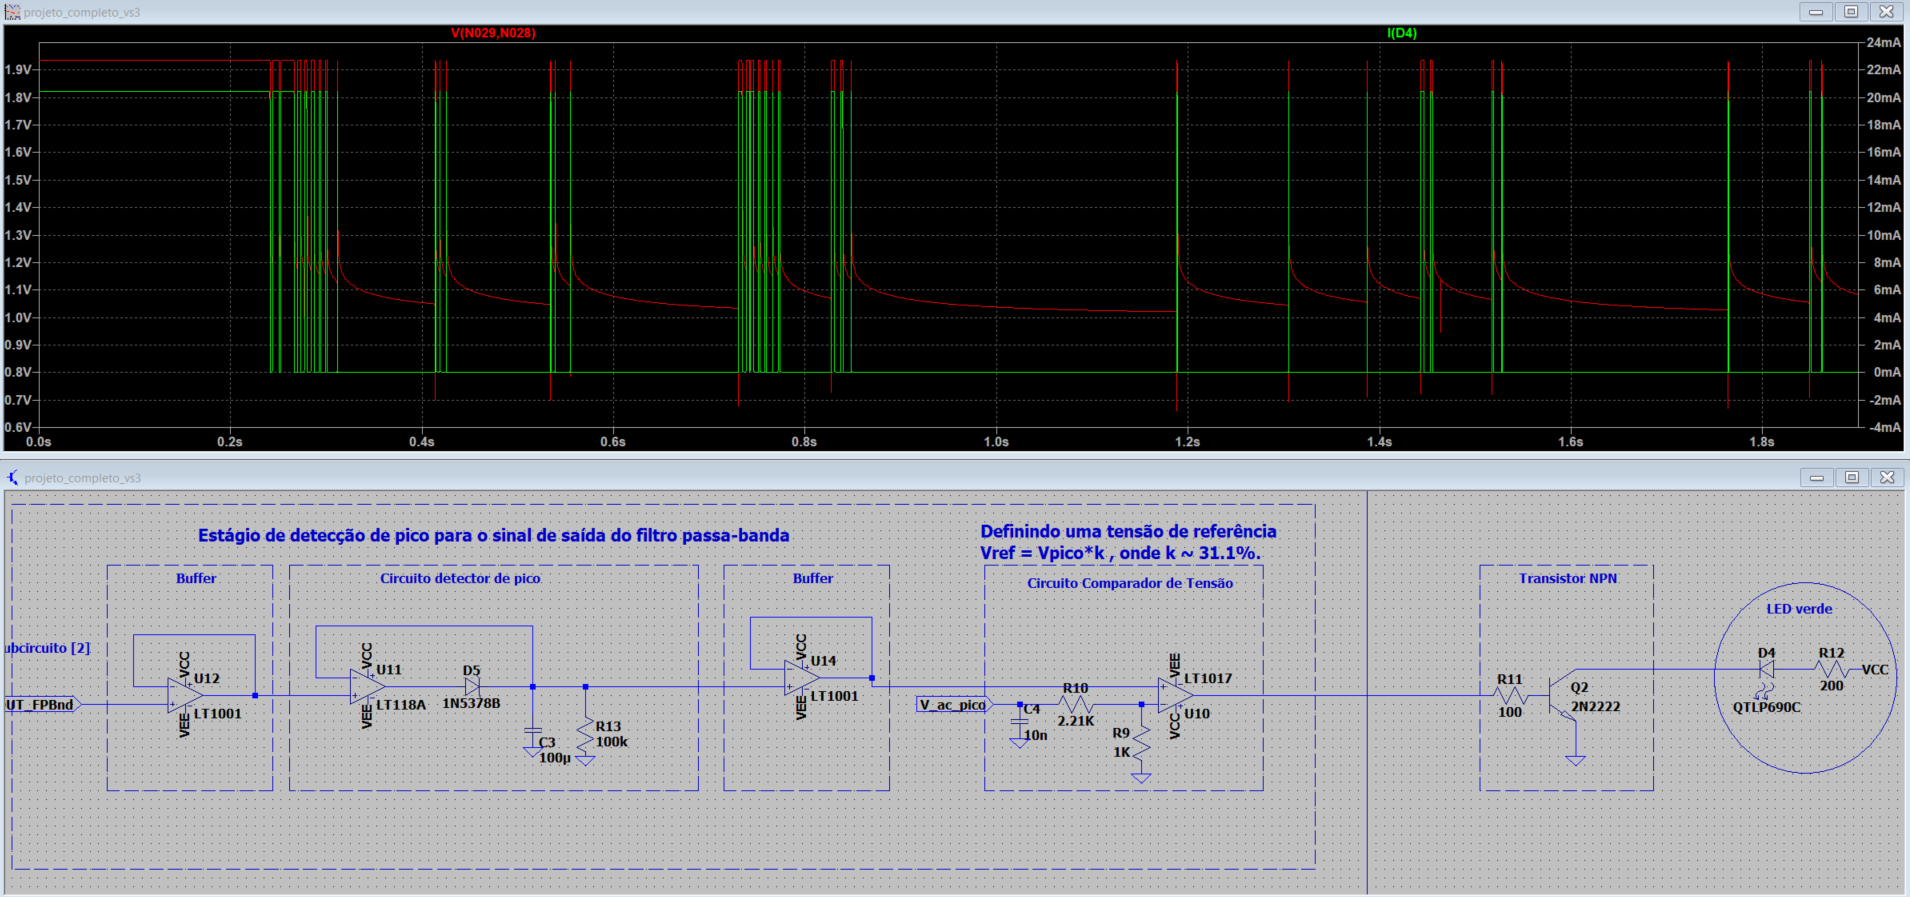
\includegraphics[scale=0.3]{imagens/graficos/simu_1v_440hz_passa-banda.png}
            \caption{Simulação do LED verde: 1V a 440hz}
        \end{figure}

        \item \textbf{f = 435hz}:
        \begin{figure}[H]
        \centering
            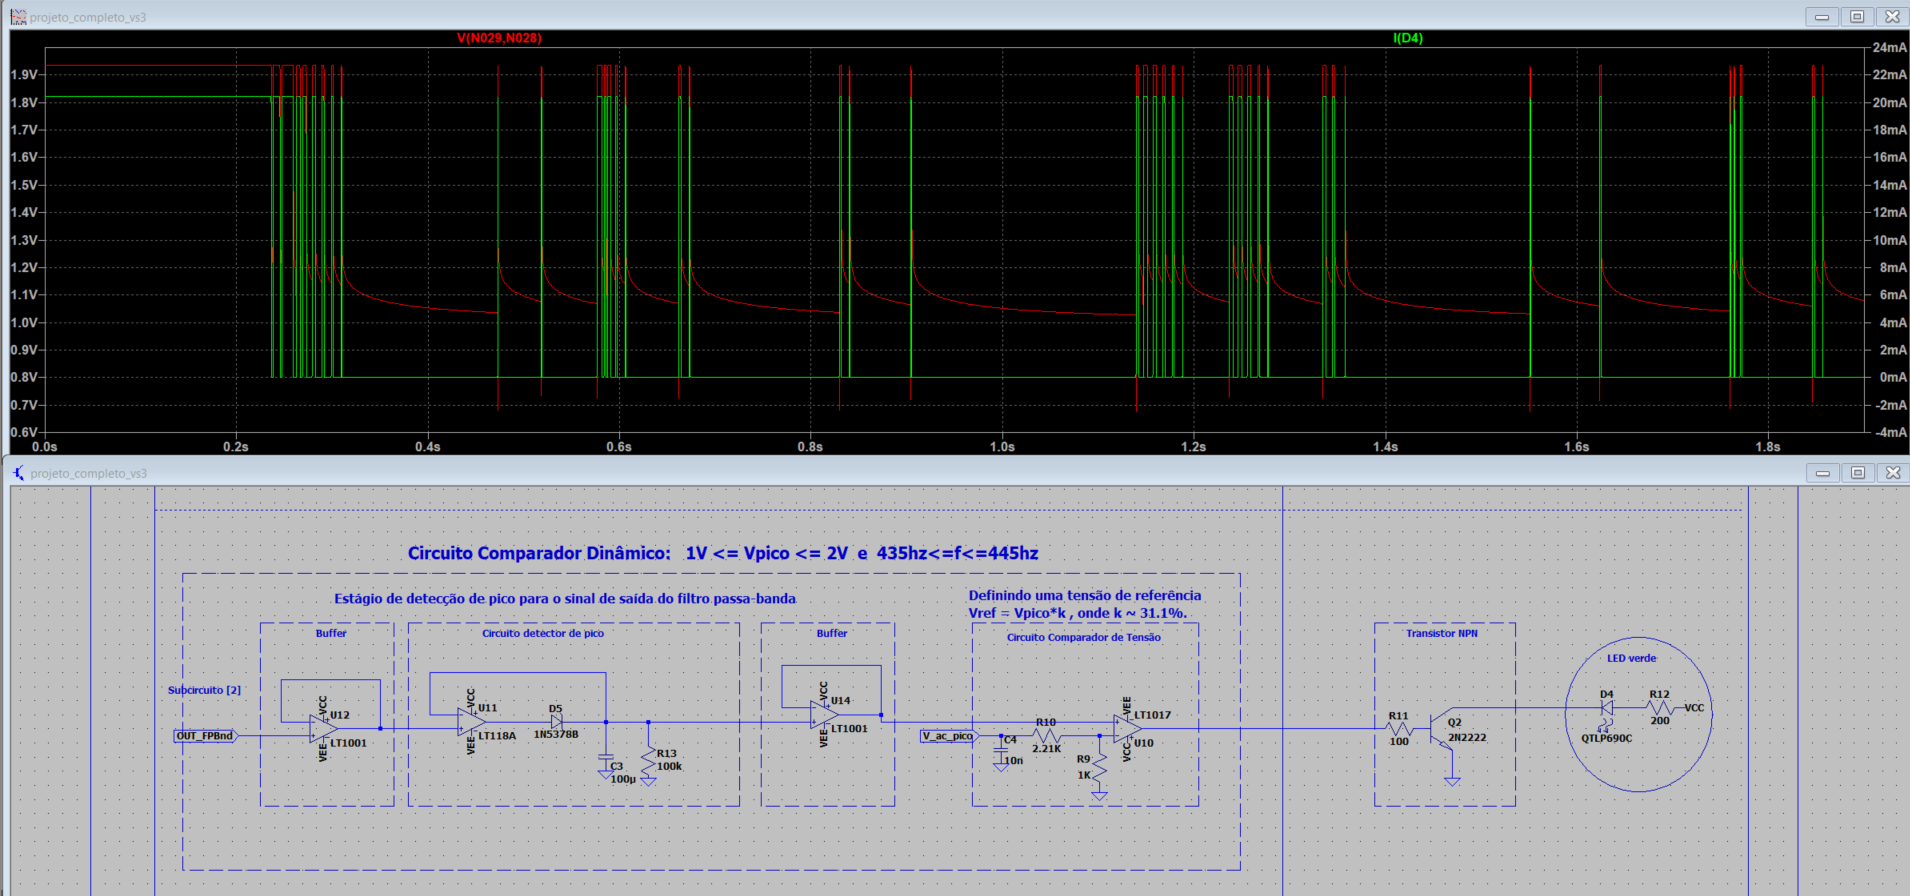
\includegraphics[scale=0.3]{imagens/graficos/simu_1v_435hz_passa-banda.png}
            \caption{Simulação do LED verde: 1V a 435hz}
        \end{figure}
    \end{itemize}

    \item \textbf{Tensão senoidal = 2V}:
    \begin{itemize}
        \item \textbf{f = 445hz}:
        \begin{figure}[H]
        \centering
            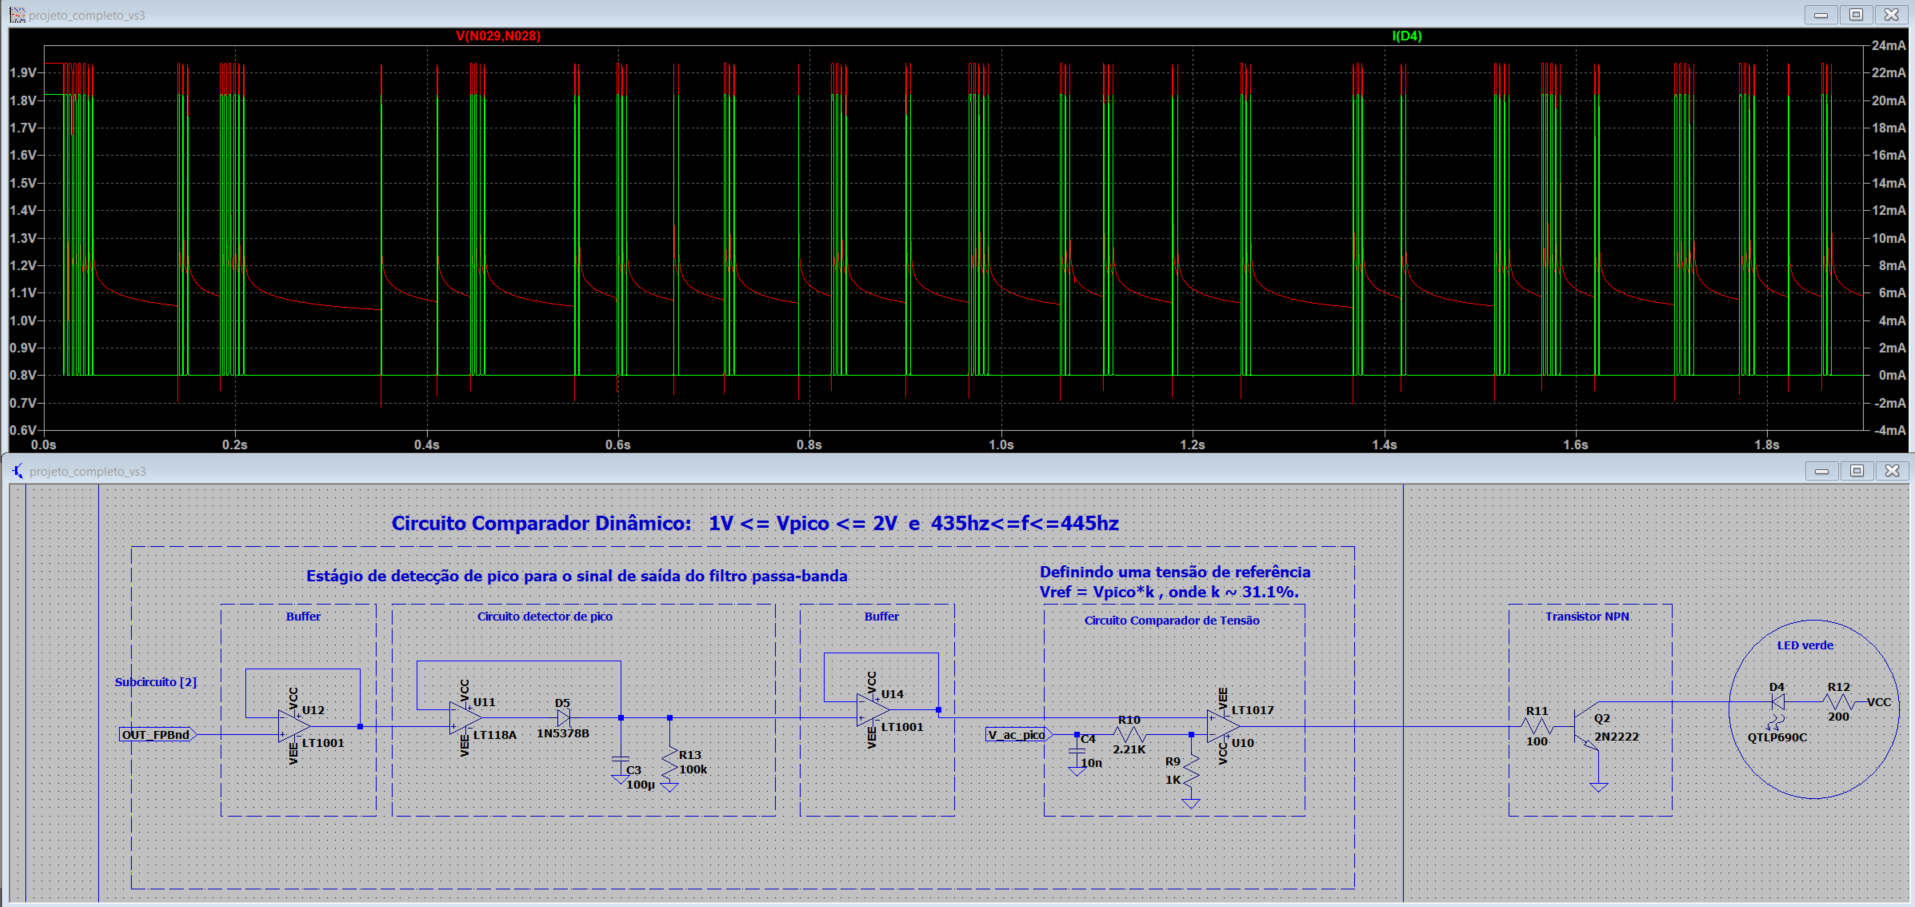
\includegraphics[scale=0.3]{imagens/graficos/simu_2v_445hz_passa-banda.png}
            \caption{Simulação do LED verde: 2V a 445hz}
        \end{figure}

        \item \textbf{f = 440hz}:
        \begin{figure}[H]
        \centering
            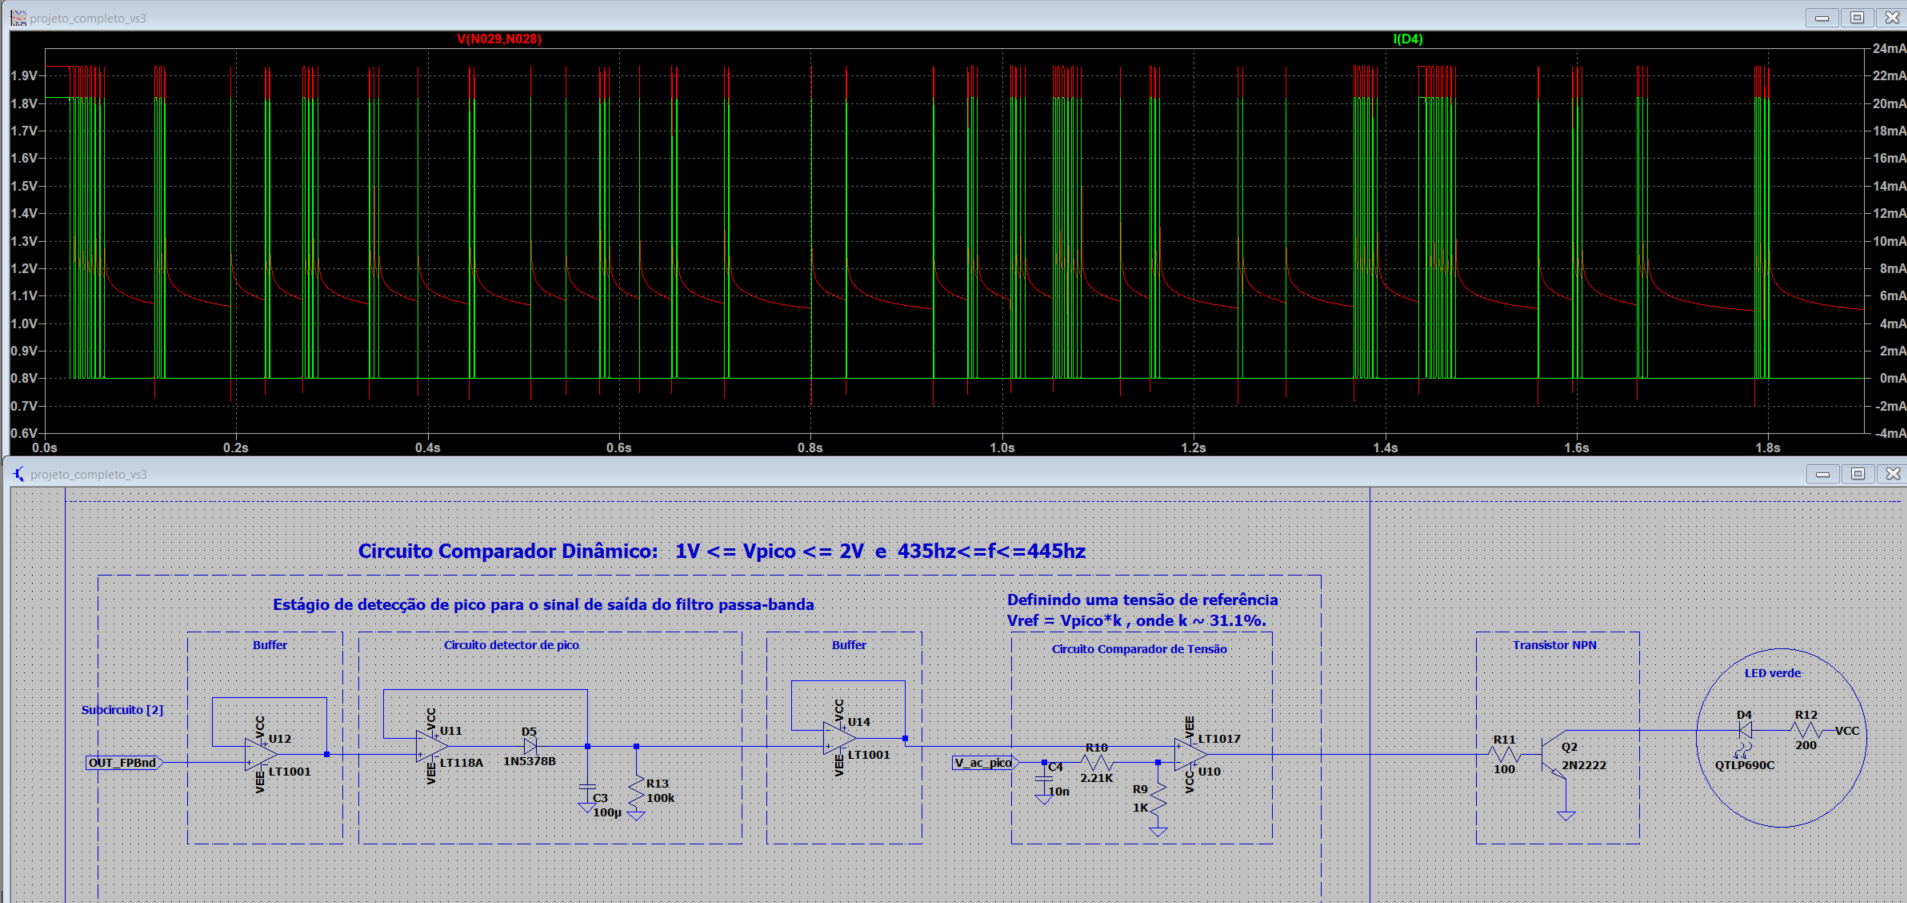
\includegraphics[scale=0.3]{imagens/graficos/simu_2v_440hz_passa-banda.png}
            \caption{Simulação do LED verde: 2V a 440hz}
        \end{figure}

        \item \textbf{f = 435hz}:
        \begin{figure}[H]
        \centering
            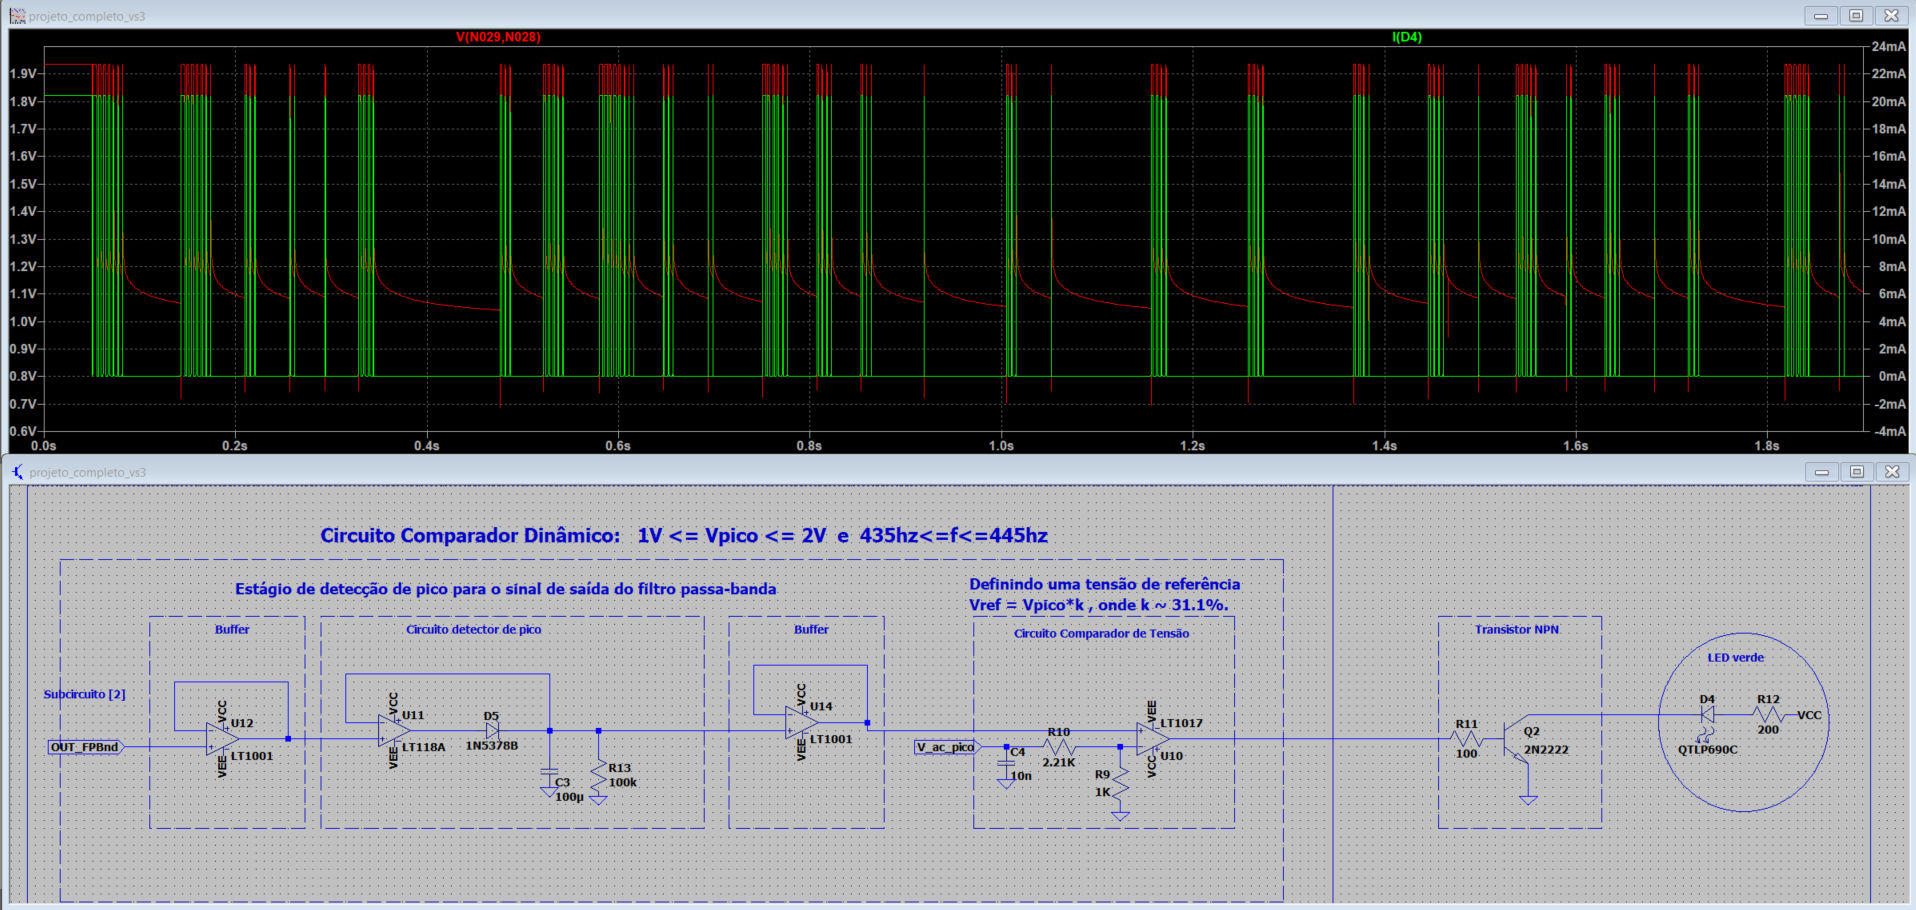
\includegraphics[scale=0.3]{imagens/graficos/simu_2v_435hz_passa-banda.png}
            \caption{Simulação do LED verde: 2V a 435hz}
        \end{figure}
    \end{itemize}
\end{itemize}




%%%%%%%%%%%%%%%%%%%%%%%%%%%%%%%%%%%%%%%%%%%%%%%%%%%%%%%%






%%%%%%%%%%%%%%%%%%%%%%%%%%%%%%%%%%%%%%%%%%%%%%%%%%%%%%%%
\newpage
\section{Conclusão}

Após os ajustes necessários e as devidas calibragens dos capacitores e resistores, além da inclusão de buffers para garantir estabilidade e isolamento dos estágios, o sistema demonstrou um desempenho eficiente e alinhado com os objetivos do projeto. \\

Os filtros Passa-Baixa e Passa-Alta se comportaram conforme projetado, delimitando com precisão as frequências de interesse: abaixo de 435 Hz e acima de 445 Hz, respectivamente. Estes filtros proporcionaram uma clara distinção das faixas de frequência, acionando os LEDs correspondentes (amarelo e vermelho) de forma consistente e sem falhas.\\

No caso do filtro Passa-Banda, devido ao estreito intervalo de frequências estipulado (435 Hz a 445 Hz), foi observado um leve ruído durante a transição de frequências. Entretanto, esse comportamento está dentro das expectativas, considerando as características do sistema. O LED verde apresentou maior intensidade luminosa em torno de 440 Hz, evidenciando que o filtro Passa-Banda cumpre sua função de identificar a frequência central com maior precisão.\\

De forma geral, o projeto demonstrou que é possível implementar um sistema eficiente de detecção e indicação de frequência utilizando técnicas de filtragem ativa, comparadores dinâmicos e drivers de LED. Apesar dos desafios associados à calibração e ao pequeno intervalo do Passa-Banda, o desempenho final atende aos requisitos propostos, validando as escolhas de projeto e os componentes empregados.


\newpage
% REFERENCIAS %%%%%%%%%%%%%%%%%%%%%%%%%%%%%%%%%%%%%%%%%%%%%%%%%%%%%%%%%%%%%%
    \nocite{*}
    \bibliography{example}
    
\end{document}
\section{Referências Bibliográficas}

